\documentclass{beamer}

\mode<presentation>

{
\usetheme{Rochester}
\setbeamercovered{transparent}
}

\usecolortheme{wolverine}

\AtBeginSection[]
{
\begin{frame}
\frametitle{Content}
\tableofcontents[currentsection]
\end{frame}
}

\usepackage{amsmath}
\usepackage{amsfonts}
\usepackage{amssymb}
\usepackage[english]{babel}
\usepackage{graphicx}
\usepackage{pict2e}
\usepackage[utf8]{inputenc}
\usepackage[T1]{fontenc}
\usepackage{color}
%\usepackage[natbib=true, style=thesis, url=false, doi=false, firstinits=true, defernumbers=true, bibstyle=numeric, title=false, sorting=ydnt, citestyle=authoryear-comp, isbn=false]{biblatex}
\usepackage{lmodern}
\usepackage{hyperref}
\usepackage{lscape}
\usepackage{multirow}
\usepackage[parfill]{parskip}
\usepackage{makeidx}
%\usepackage{times}
%\bibliography{library}
\usepackage{wrapfig}
\usepackage{pgf}
\usepackage{fancybox}
\usepackage{multimedia}
%\usepackage[]{movie15}

\definecolor{white}{gray}{1}
\def\wct#1{\textcolor{white}{#1}}
\definecolor{orange}{RGB}{255,165,0}
\definecolor{aquamarine}{RGB}{127,255,212}
\definecolor{dodger}{RGB}{30,144,255}

\newcommand{\obs}{\mathrm{obs}}
\newcommand{\pred}{\mathrm{pred}}
\newcommand{\eff}{\mathrm{eff}}
\newcommand{\intt}{\mathrm{int}}
\newcommand{\LMC}{\mathrm{LMC}}
\newcommand{\MW}{\mathrm{MW}}
\newcommand{\Cepheid}{\mathrm{Cepheid}}
\newcommand{\Anchors}{\mathrm{Anchors}}
\newcommand{\SNe}{\mathrm{SNe\,Ia}}
\newcommand{\km}{\mathrm{km}}
\newcommand{\second}{\mathrm{s}}
\newcommand{\Mpc}{\mathrm{Mpc}}
\newcommand{\MAnd}{\mathrm{M31}}
\newcommand{\NGC}{\mathrm{NGC4258}}
%\def\be{\begin{equation}}
%\def\ee{\end{equation}}
%\def\bea{\begin{eqnarray}}
%\def\eea{\end{eqnarray}}


\author[Wilmar Alberto Cardona Castro]{Wilmar Alberto Cardona Castro}
%\institute[]{University of Geneva}
%\date{18th June, 2012}

\title[A new measurement of the Hubble constant]{A new measurement of the Hubble constant}
\subject{Cosmology}

\setbeamercolor{frametitle}{bg=dodger}
\beamerdefaultoverlayspecification{<+->}
\setbeamertemplate{footline}[frame number]
\begin{document}

\begin{frame}
%\begin{center}
%\\
%\vspace{1cm}
%\\
%\vspace{1cm}
%\\
%\vspace{1cm}
%
%\end{center}
\begin{figure}[hbtp]
\centering
\setlength{\unitlength}{0.1\textwidth}
\begin{picture}(10,7)
\put(0,0){
\includegraphics[scale=0.5]{UNIGE50.jpg}}
\put(1,6){\textbf{Cosmological constraints: anisotropic dark energy,}}
\put(1.5,5.5){\textbf{the Hubble constant, and the neutrino mass}}
\put(2.5,4){Wilmar Alberto Cardona Castro}
\put(3.,2.5){Supervisor: Martin Kunz}
\put(3.4,1){September 27, 2016}
\end{picture}
\end{figure}

\end{frame}

\begin{frame}
\begin{itemize}
\item \textbf{The traces of anisotropic dark energy in light of Planck} in collaboration with Lukas Hollenstein and Martin Kunz
\item \textbf{Lensing convergence and the neutrino mass scale in galaxy redshift surveys} in collaboration with Ruth Durrer, Martin Kunz, and Francesco Montanari
\item \textbf{Testing isotropy and Gaussianity in the Planck CMB estimates}
\item \textbf{Determining $H_0$ with Bayesian hyper-parameters} in collaboration with Martin Kunz and Valeria Pettorino 
\end{itemize}
\end{frame}

\begin{frame}
  \titlepage
\end{frame}

\begin{frame}{Content}
  \tableofcontents
\end{frame}

\section{Introduction}

\begin{frame}{The concordance model of cosmology}
\begin{figure}[hbtp]
\centering
\setlength{\unitlength}{0.1\textwidth}
\begin{picture}(10,7)
\only<1-4>{
\put(0,5){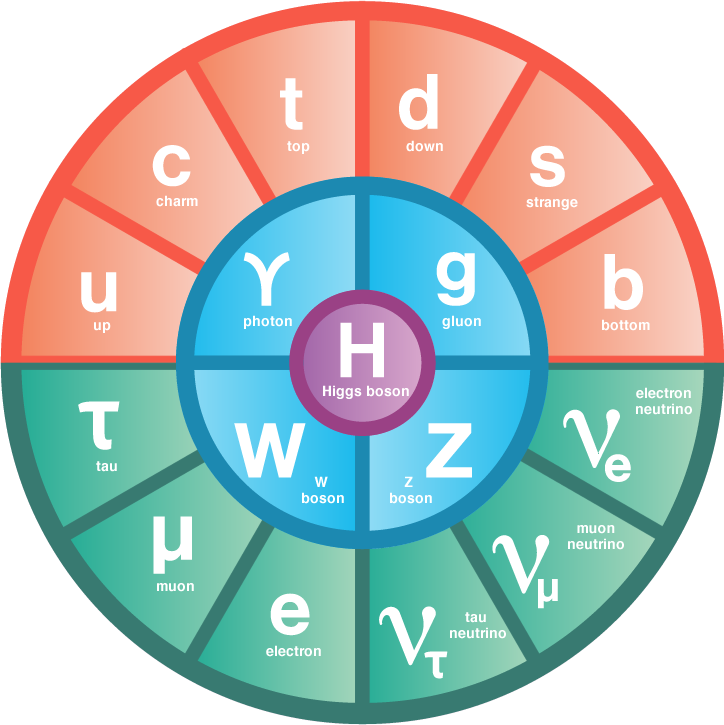
\includegraphics[width=0.2\textwidth]{../figures/standard_model_ai_s2.png}}
\put(3,4.7){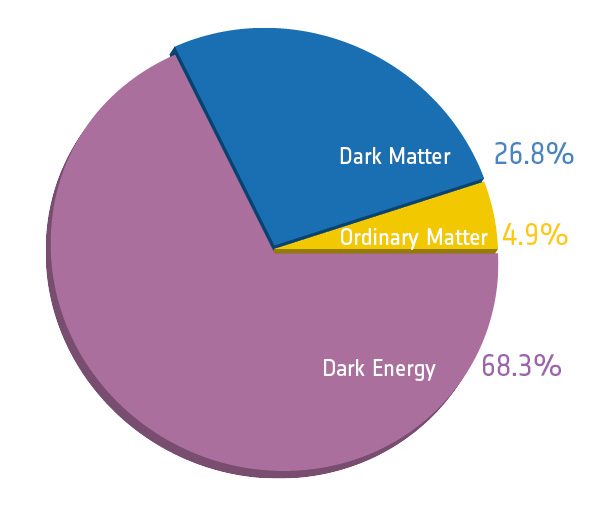
\includegraphics[scale=0.15]{../figures/Planck-only_Cosmic-recipe-pie-chart.jpg}}
\put(0,2.5){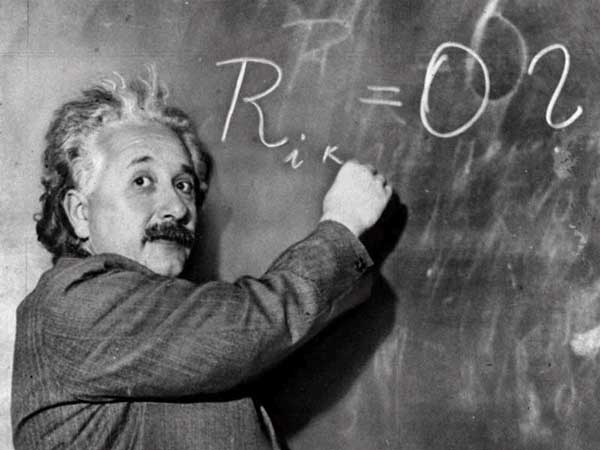
\includegraphics[scale=0.15]{albert-einstein21.jpg}}
\put(3.8,4.3){Inflation}}
\only<1-4>{
\put(3.8,3.8){Cold Dark Matter}}
\only<1-4>{
\put(3.8,3.3){$w=-1$}}
\only<1-4>{
\put(3.8,2.8){Flatness}}
\only<2-4>{
\put(1,2){$\Omega_{\rm cdm}$, $\Omega_b$, $n_s$, $A_s$, $\tau$, $\mathbf{H_0}$}}

\only<3-4>{
\put(7,5){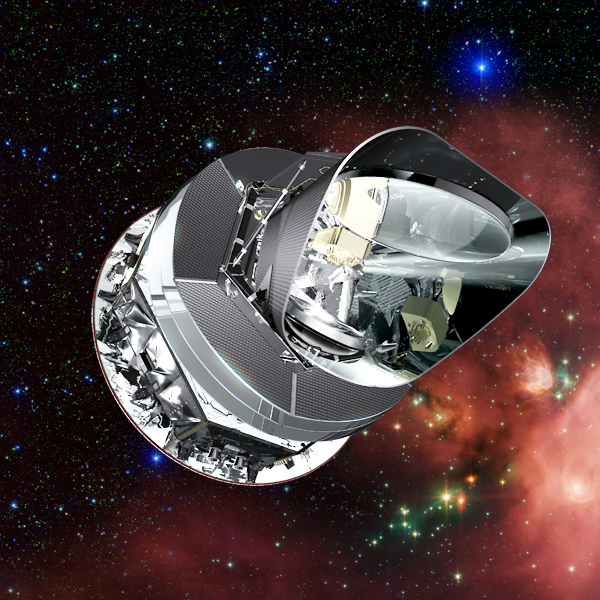
\includegraphics[scale=0.12]{Planck-600x600.jpg} }
\put(7,2.8){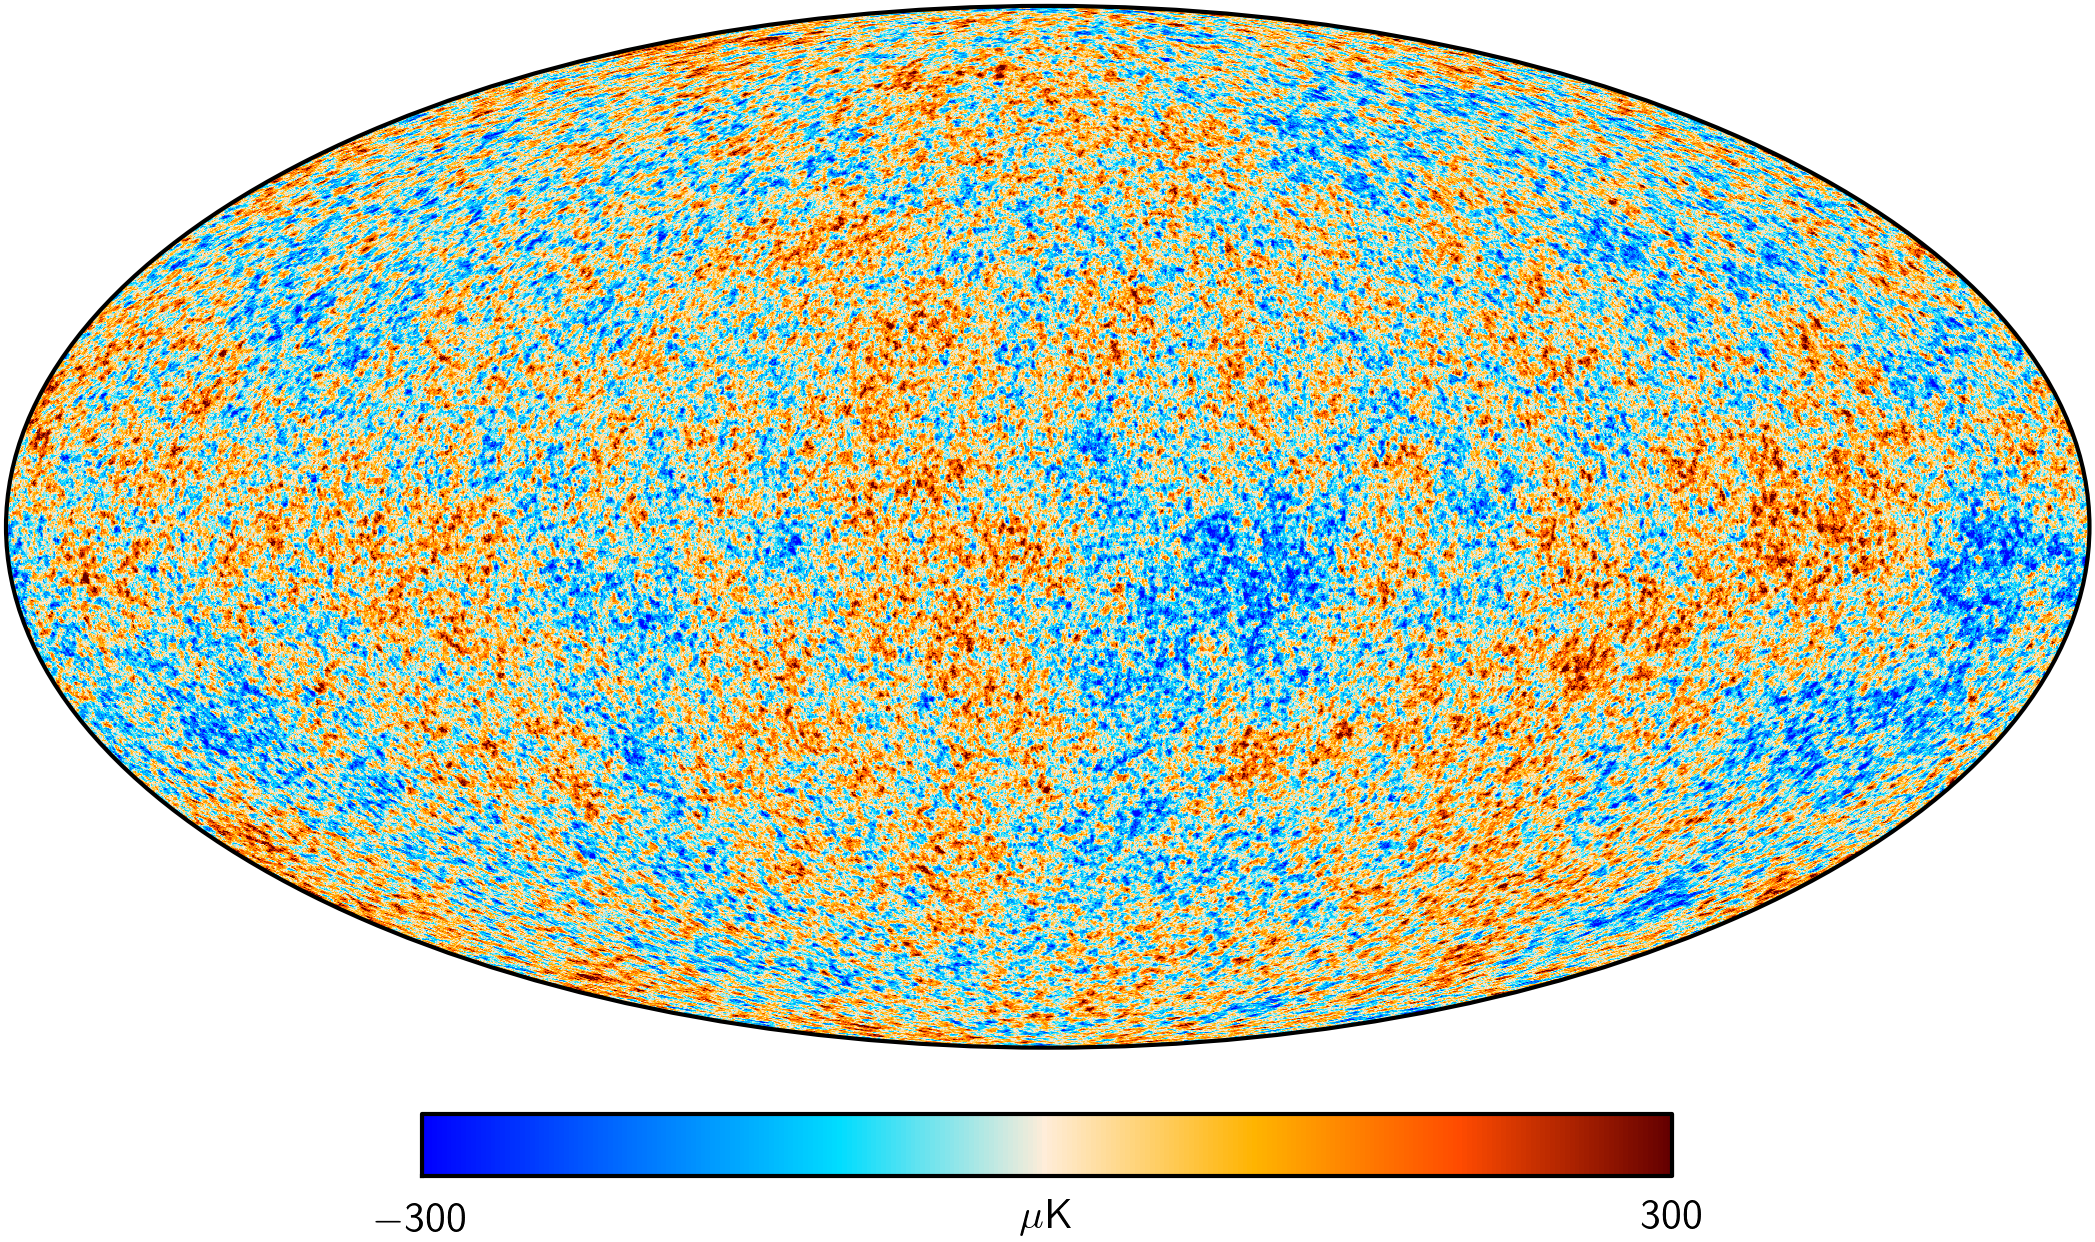
\includegraphics[width=0.3\textwidth]{../figures/2015_SMICA_CMB.png}}}

\only<4>{
\put(0,1){Statistical properties}
\put(0,0.5){of the model}
\put(7,1){Statistical properties}
\put(7,0.5){of the data}}
\end{picture}
\end{figure}
\end{frame}

\begin{frame}{A good phenomenological description of the Universe}
\begin{figure}[hbtp]
\centering
\setlength{\unitlength}{0.1\textwidth}
\begin{picture}(10,7)
\put(0,0.5){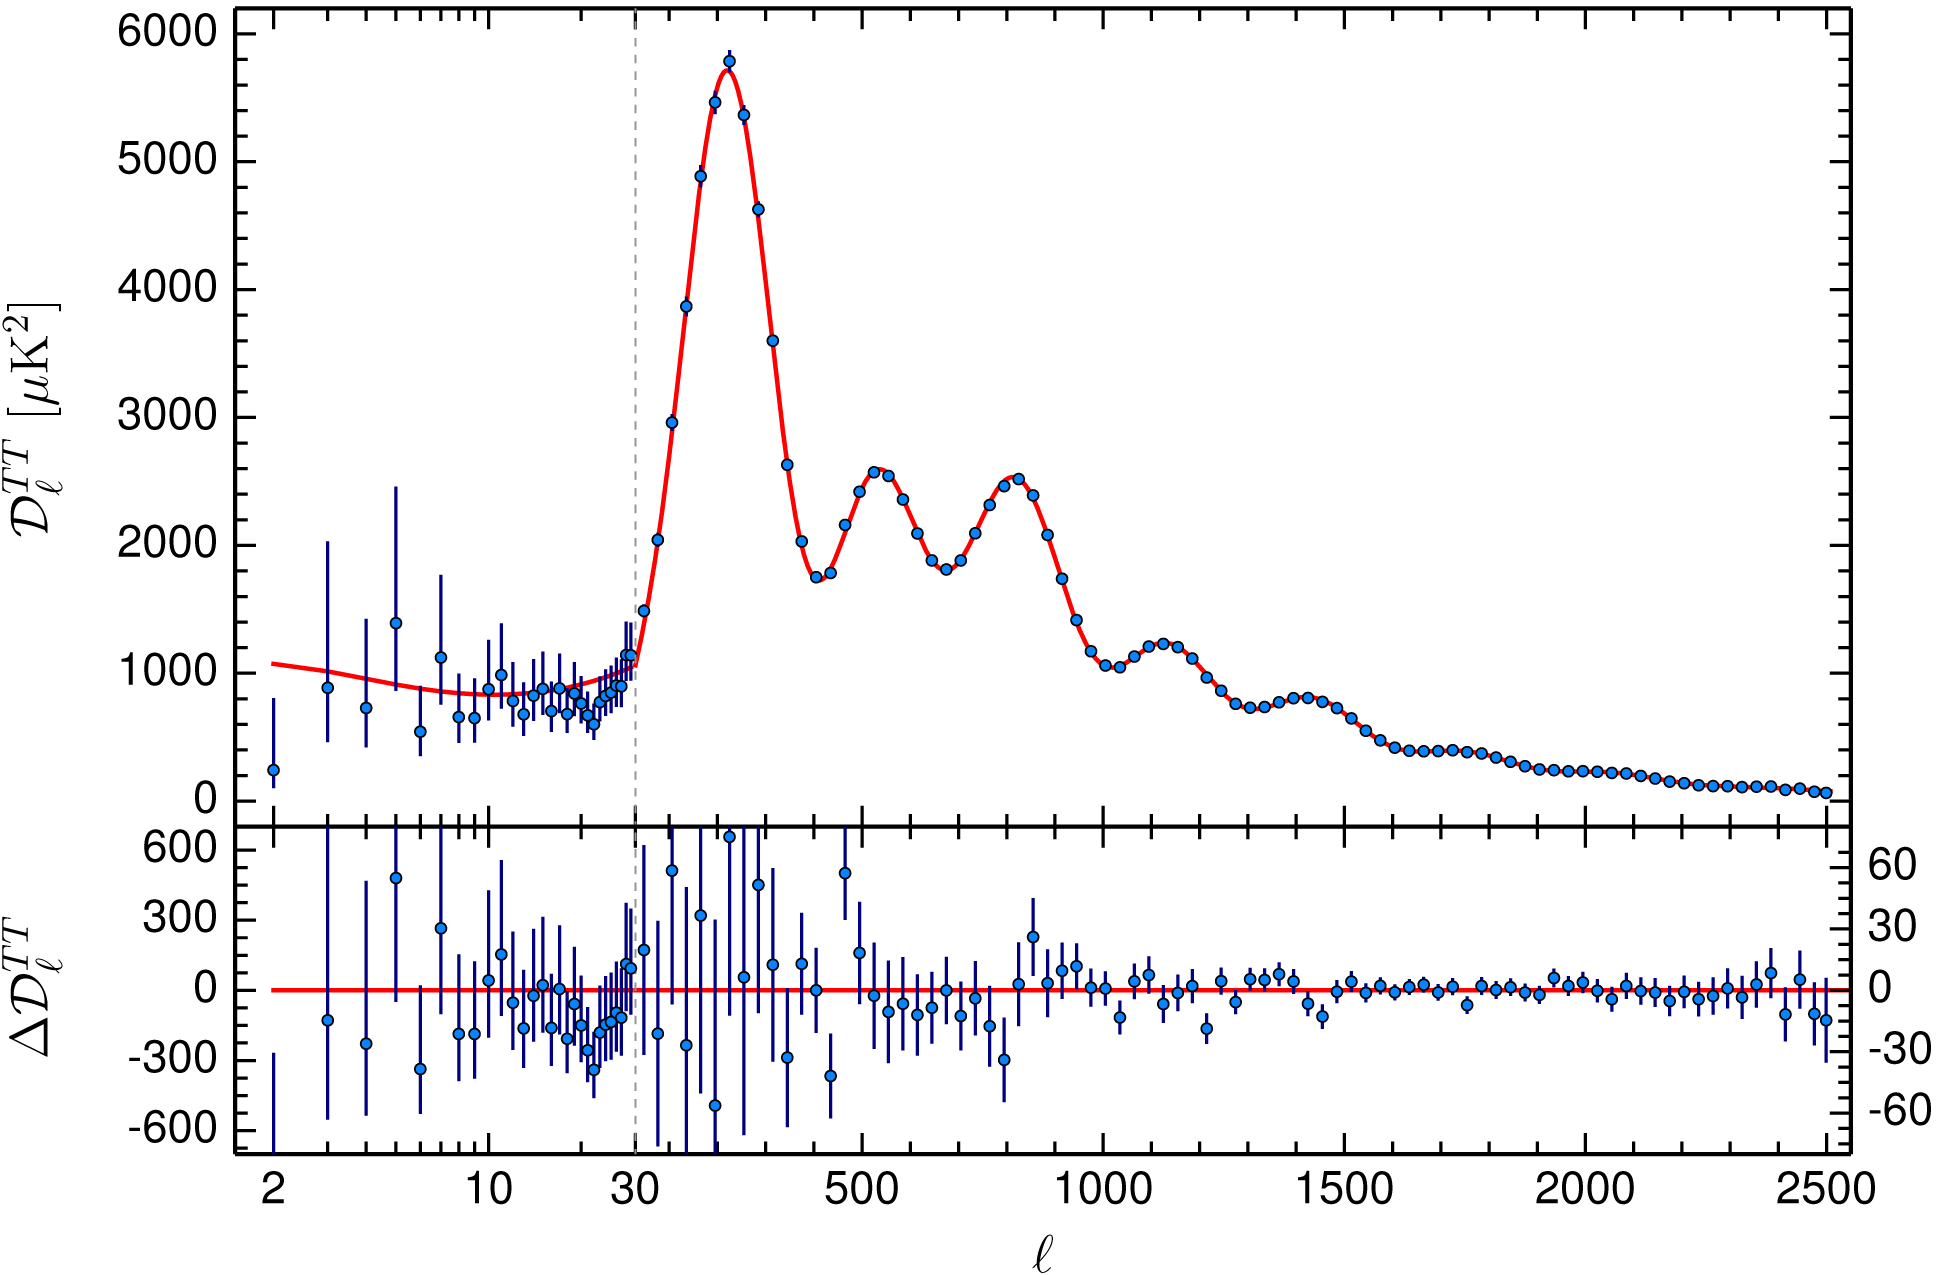
\includegraphics[width=\textwidth]{../figures/2015_TTSpectrum.png}}
\put(4.4,6){$H_0=66.93\pm0.62\, \km\, \second^{-1}\, \Mpc^{-1}$}
\put(0,0){Credit:Planck Collaboration}
\end{picture}
\end{figure}
\end{frame}

\begin{frame}{Why do we care about a local measurement of $H_0$?}
\only<1-2>{\begin{figure}[hbtp]
\centering
\setlength{\unitlength}{0.1\textwidth}
\begin{picture}(10,7)
\put(-0.5,2.5){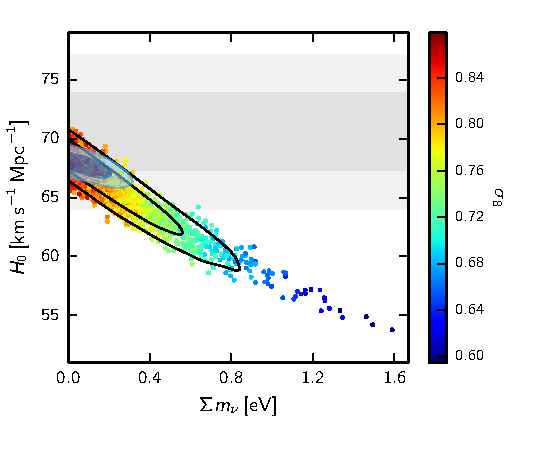
\includegraphics[scale=0.65]{../figures/chapter-h0/mnu-H0.pdf}
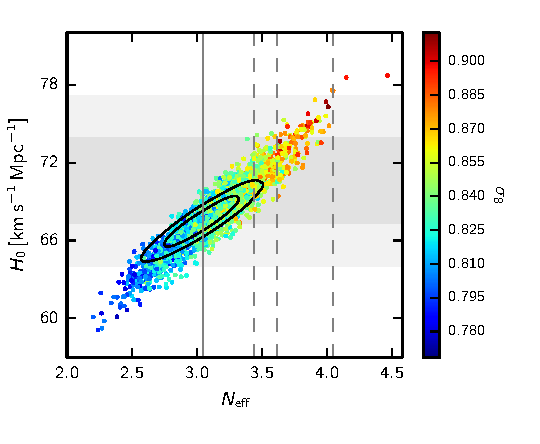
\includegraphics[scale=0.65]{../figures/chapter-h0/Neff-H0.pdf}}
\put(0,7){Credit:Planck Collaboration}
\only<1>{
%\item
\put(0,2){Cosmological scales and break degeneracies:}
\put(0,1.5){crucial for understanding the standard model of cosmology}}
\only<2>{
%\item 
\put(0,2){Inferred determinations are model dependent (i.e., on properties of}
\put(0,1.5){neutrinos, theory of gravity, nature of dark energy, etc.) and}
\put(0,1){might be affected by assumed prior probability distributions}}
\end{picture}
\end{figure}}
\end{frame}

\begin{frame}{Recent direct and inferred determinations of $H_0$}
\only<1>{
\begin{figure}[hbtp]
\centering
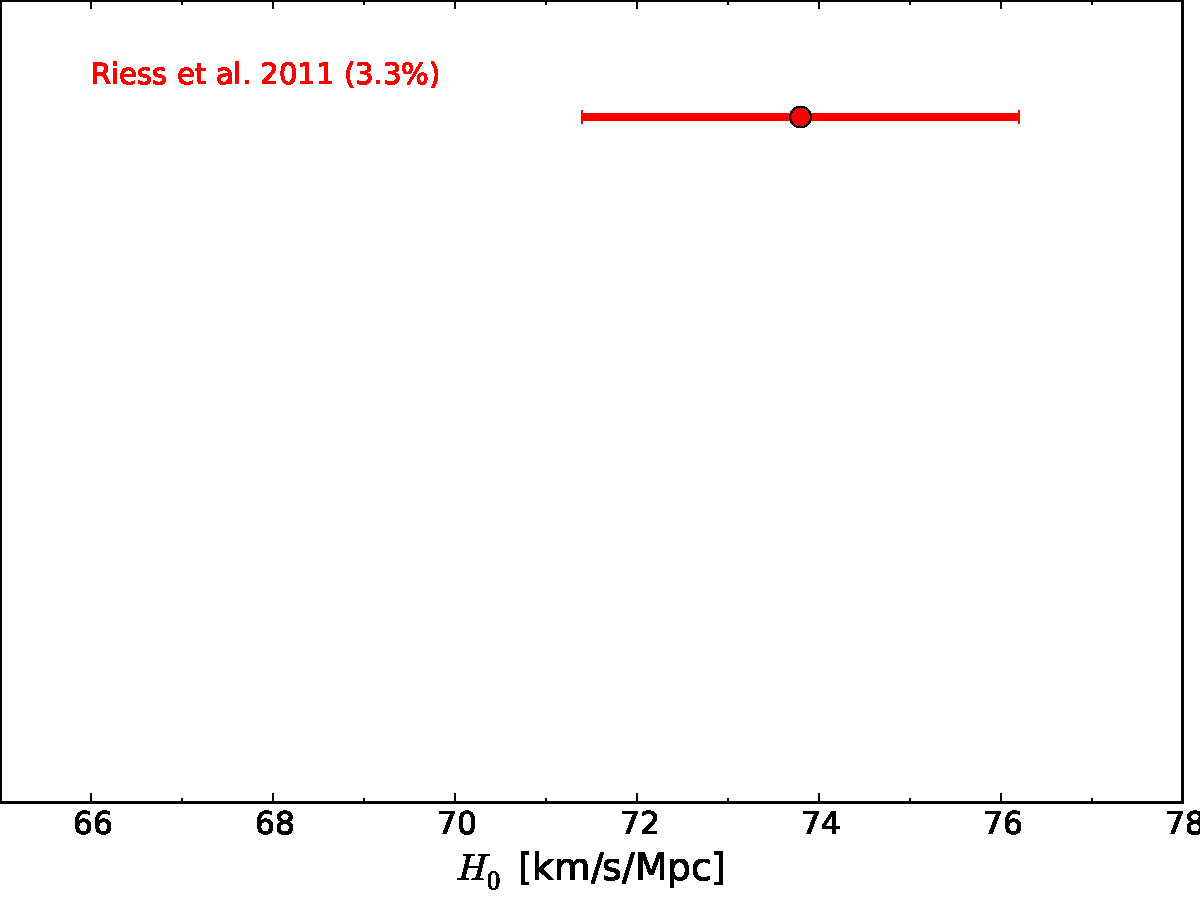
\includegraphics[width=\textwidth]{../figures/chapter-h0/H0_history-1.pdf}
\end{figure}
}
\only<2>{
\begin{figure}[hbtp]
\centering
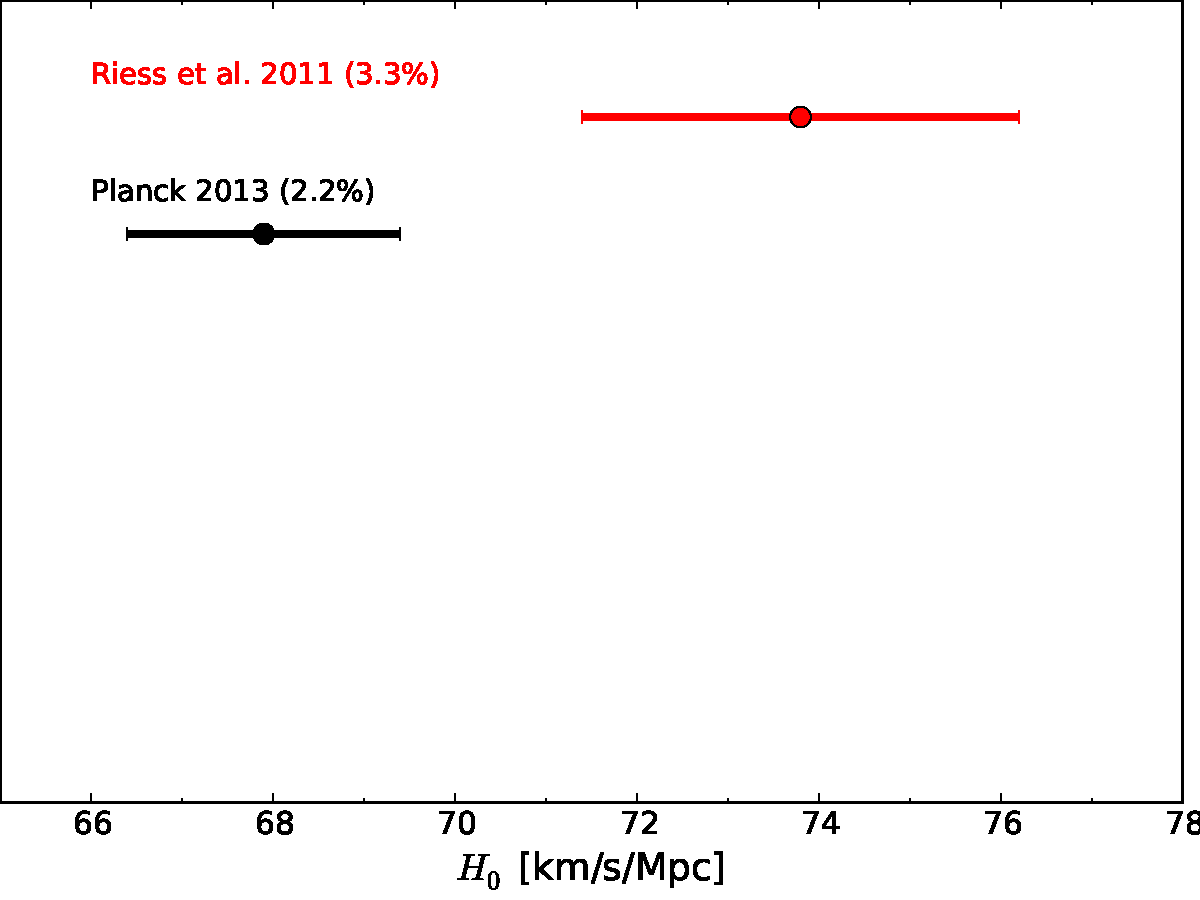
\includegraphics[width=\textwidth]{../figures/chapter-h0/H0_history-2.pdf}
\end{figure}
}
\only<3>{
\begin{figure}[hbtp]
\centering
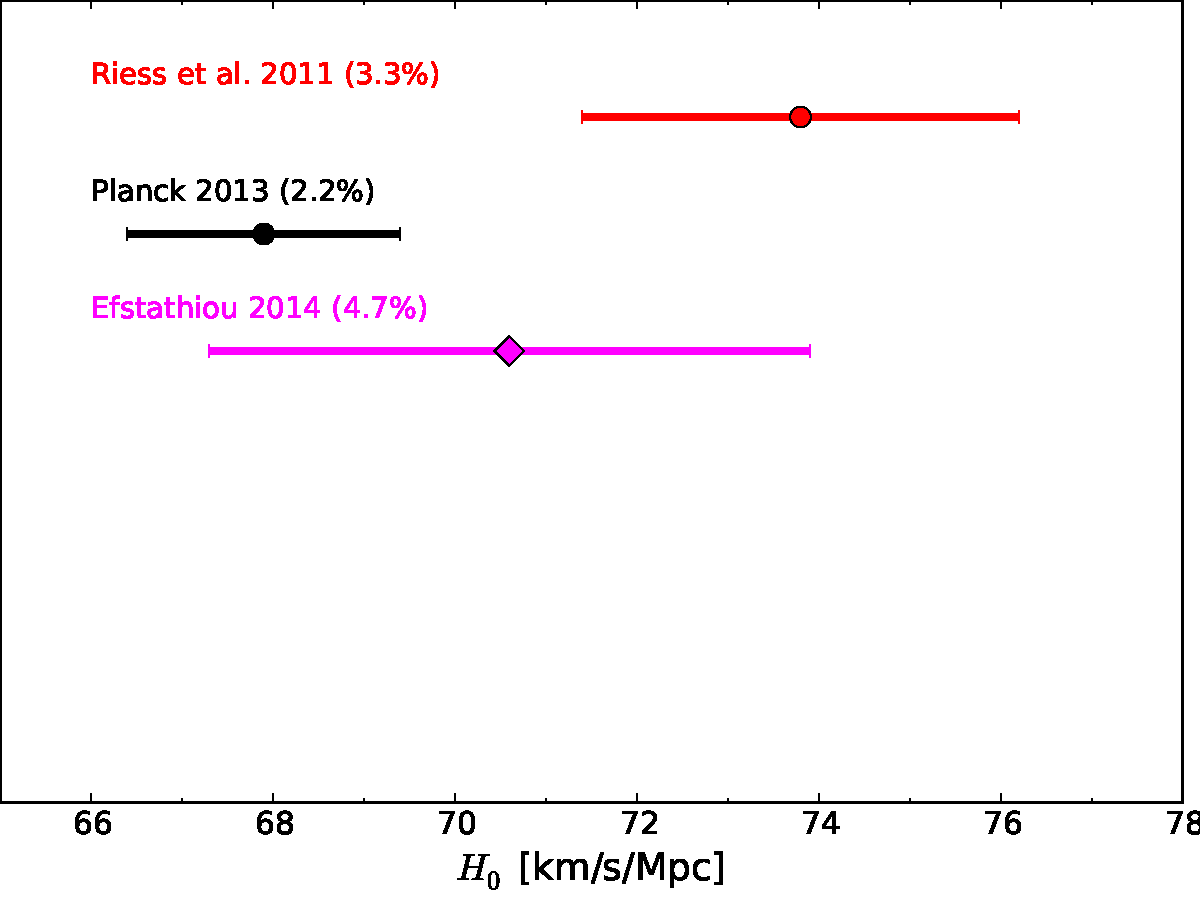
\includegraphics[width=\textwidth]{../figures/chapter-h0/H0_history-3.pdf}
\end{figure}
}
\only<4>{
\begin{figure}[hbtp]
\centering
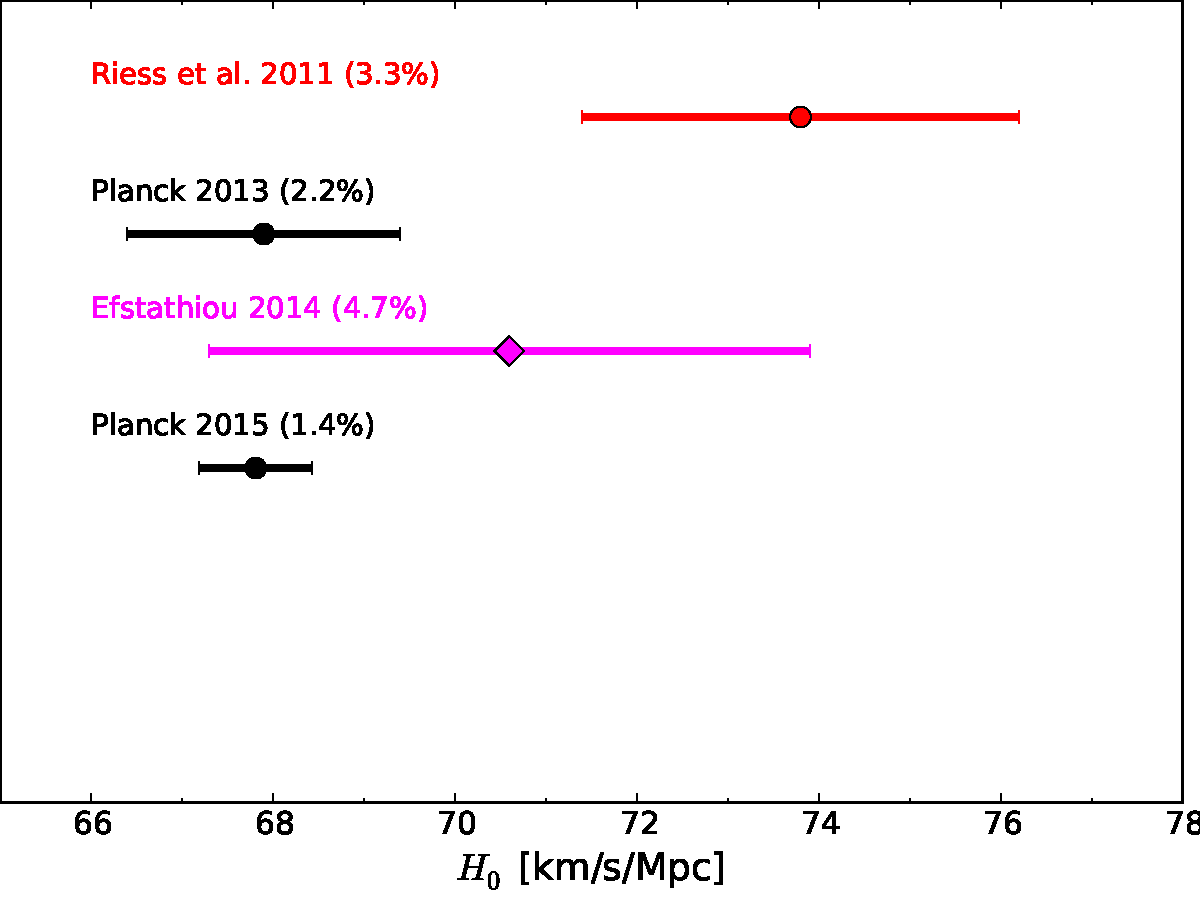
\includegraphics[width=\textwidth]{../figures/chapter-h0/H0_history-4.pdf}
\end{figure}
}
\only<5>{
\begin{figure}[hbtp]
\centering
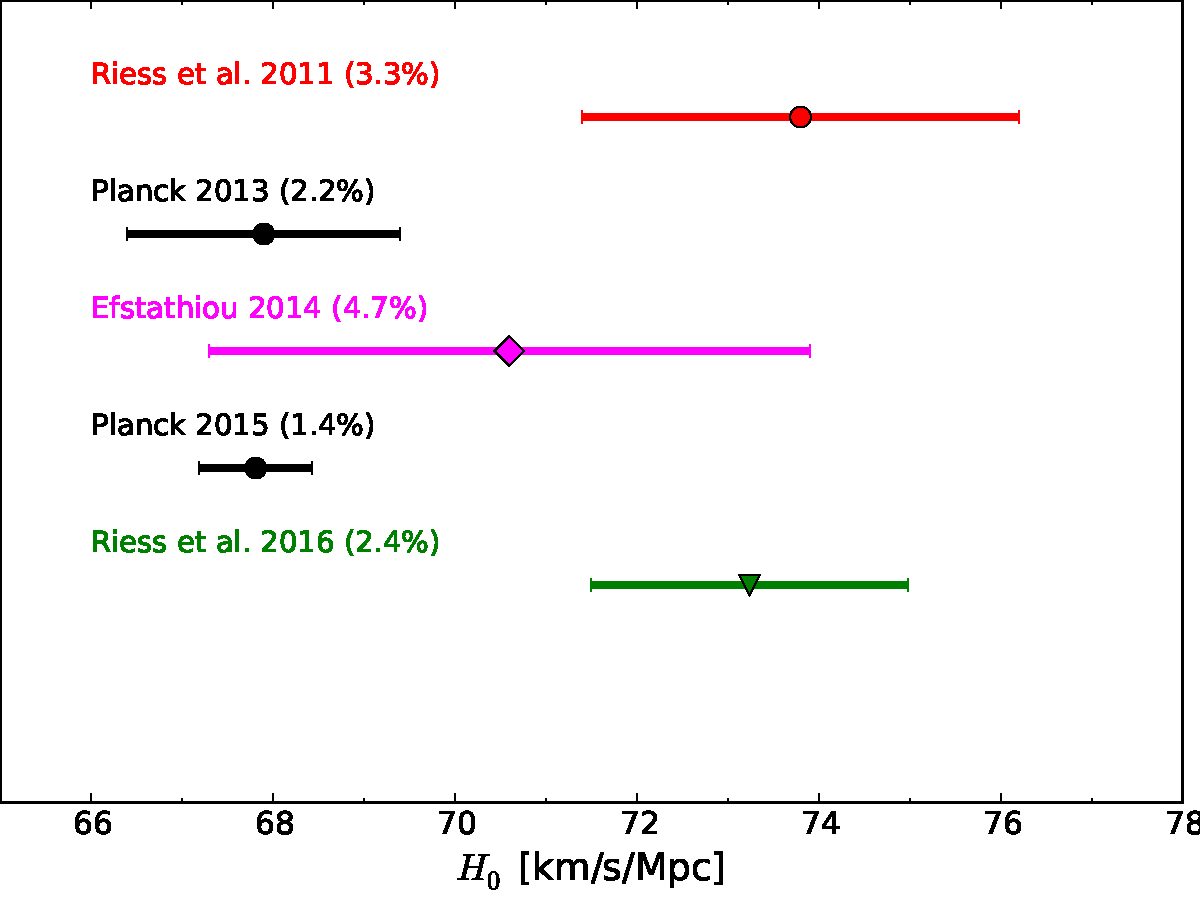
\includegraphics[width=\textwidth]{../figures/chapter-h0/H0_history-5.pdf}
\end{figure}
}
\only<6>{
\begin{figure}[hbtp]
\centering
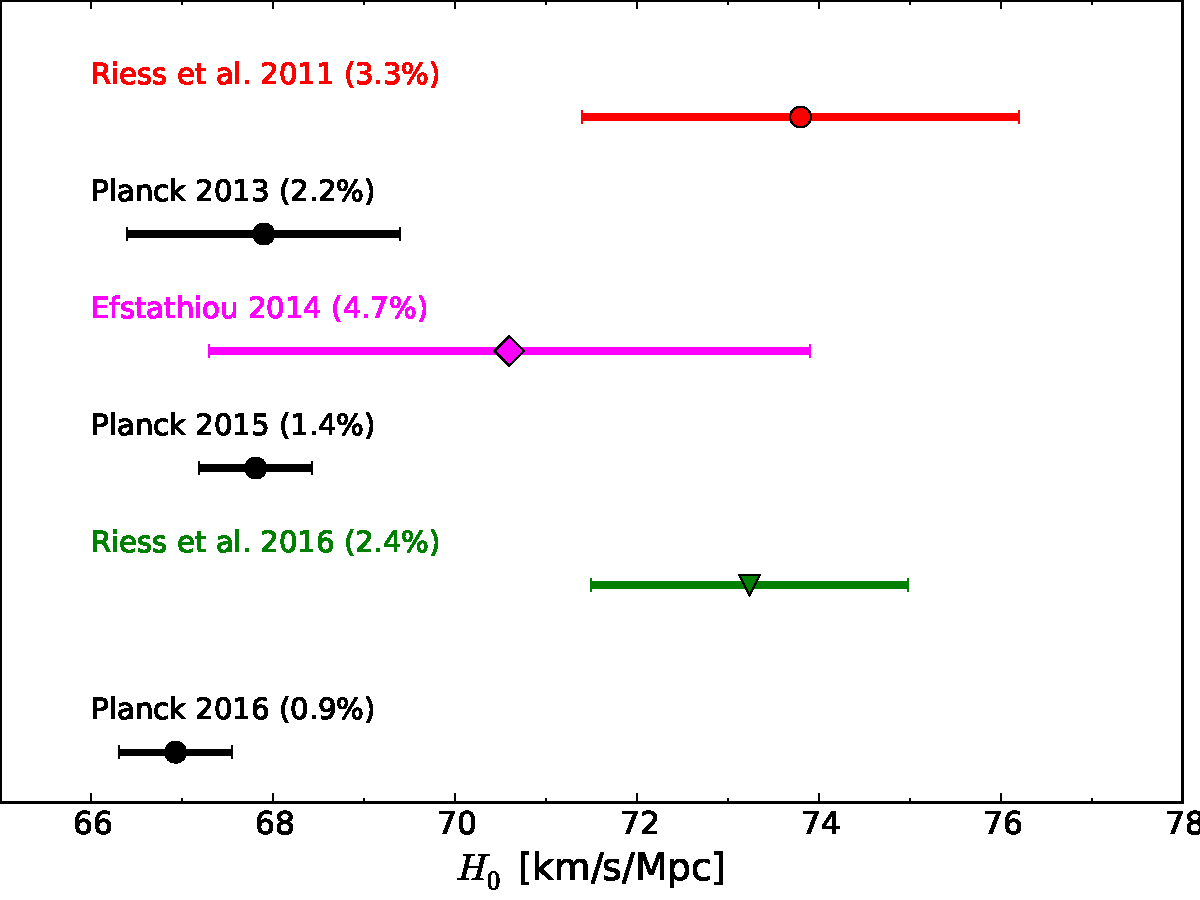
\includegraphics[width=\textwidth]{../figures/chapter-h0/H0_history.pdf}
\end{figure}
}
\only<7-10>{\begin{figure}[hbtp]
\centering
\setlength{\unitlength}{0.1\textwidth}
\begin{picture}(10,7)
\put(0.5,2){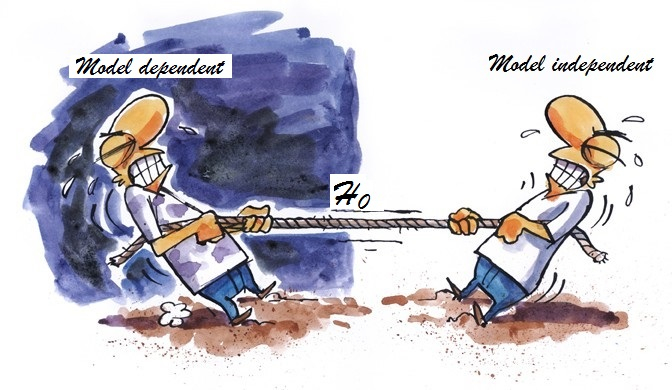
\includegraphics[scale=0.4]{../figures/chapter-h0/dependent-vs-independent.jpg}}
\only<7>{
\put(0,1.5){Interesting: there is a $\mathbf{3.4\sigma}$ \textbf{tension} between direct (\textbf{Riess et al. 2016})}
\put(0,1){and inferred (\textbf{Planck Collaboration 2016}) determinations of $H_0$.}
\put(0,0.5){At least two possible reasons.}}
\only<8>{
\put(0,1.5){1. \textbf{New physics} (e.g., modifying assumptions in the concordance}
\put(0,1){model)?}}
%\put(0,1){contributions of the local gravitational potential, unaccounted}
%\put(0,0.5){second-order corrections to the background distance-redshift relation? }}
\only<9>{
\put(0,1.5){2. \textbf{Issues with statistical analysis} (e.g., \textbf{outlier rejection algorithms},}
\put(0,1){\textbf{anchors choice}, \textbf{period cut-off} and assumptions in the Leavitt law,}
\put(0,0.5){unaccounted systematics)?}}
\only<10>{ 
\put(0,1.5){Need to confirm $\mathbf{3.4\sigma}$ \textbf{tension} and prove it \textbf{robust against}}
\put(0,1){\textbf{different statistical approaches}.}}
\end{picture}
\end{figure}}

\end{frame}

\setbeamercolor{frametitle}{bg=aquamarine}

\section{Measuring the Hubble constant}

\begin{frame}{Standard candles}
\begin{figure}[hbtp]
\centering
\setlength{\unitlength}{0.1\textwidth}
\begin{picture}(10,7)
\only<1-2>{\put(-0.5,4.5){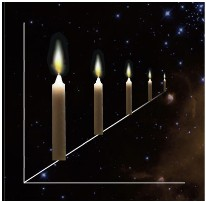
\includegraphics[scale=0.4]{../figures/chapter-h0/light-candles.jpg}}
\put(3.5,6){Distance modulus}
\put(3.5,5.5){
$\mu_0 \equiv m - M = 5 \log_{10} \left(\frac{d_L}{1 \mathrm{Mpc}} \right) + 25$
}}
\only<2>{
\put(0,4){Exploding stars:}
\put(0,3.5){Supernovae type Ia}
\put(-0.5,0.5){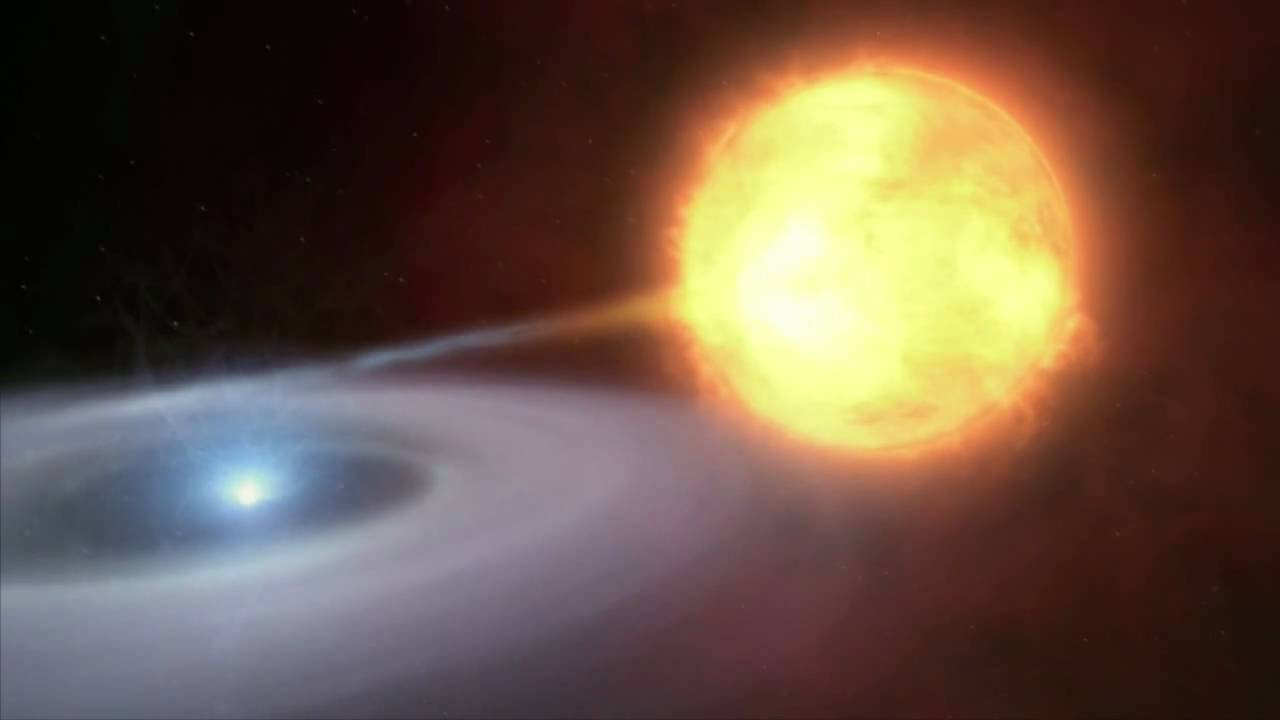
\includegraphics[scale=0.109]{../figures/chapter-h0/sntypeia.jpg}} 
\put(5,0.5){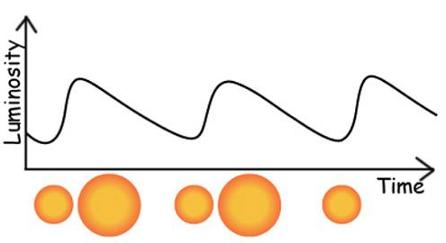
\includegraphics[scale=0.45]{../figures/chapter-h0/cepheid.jpg}}
\put(5.5,4){Pulsating stars:}
\put(5.5,3.5){Cepheid variables}}
\end{picture}
\end{figure}
\end{frame}

\begin{frame}{How do we measure $H_0$?}
\begin{figure}[hbtp]
\centering
\setlength{\unitlength}{0.1\textwidth}
\begin{picture}(10,7)
\put(0,0.5){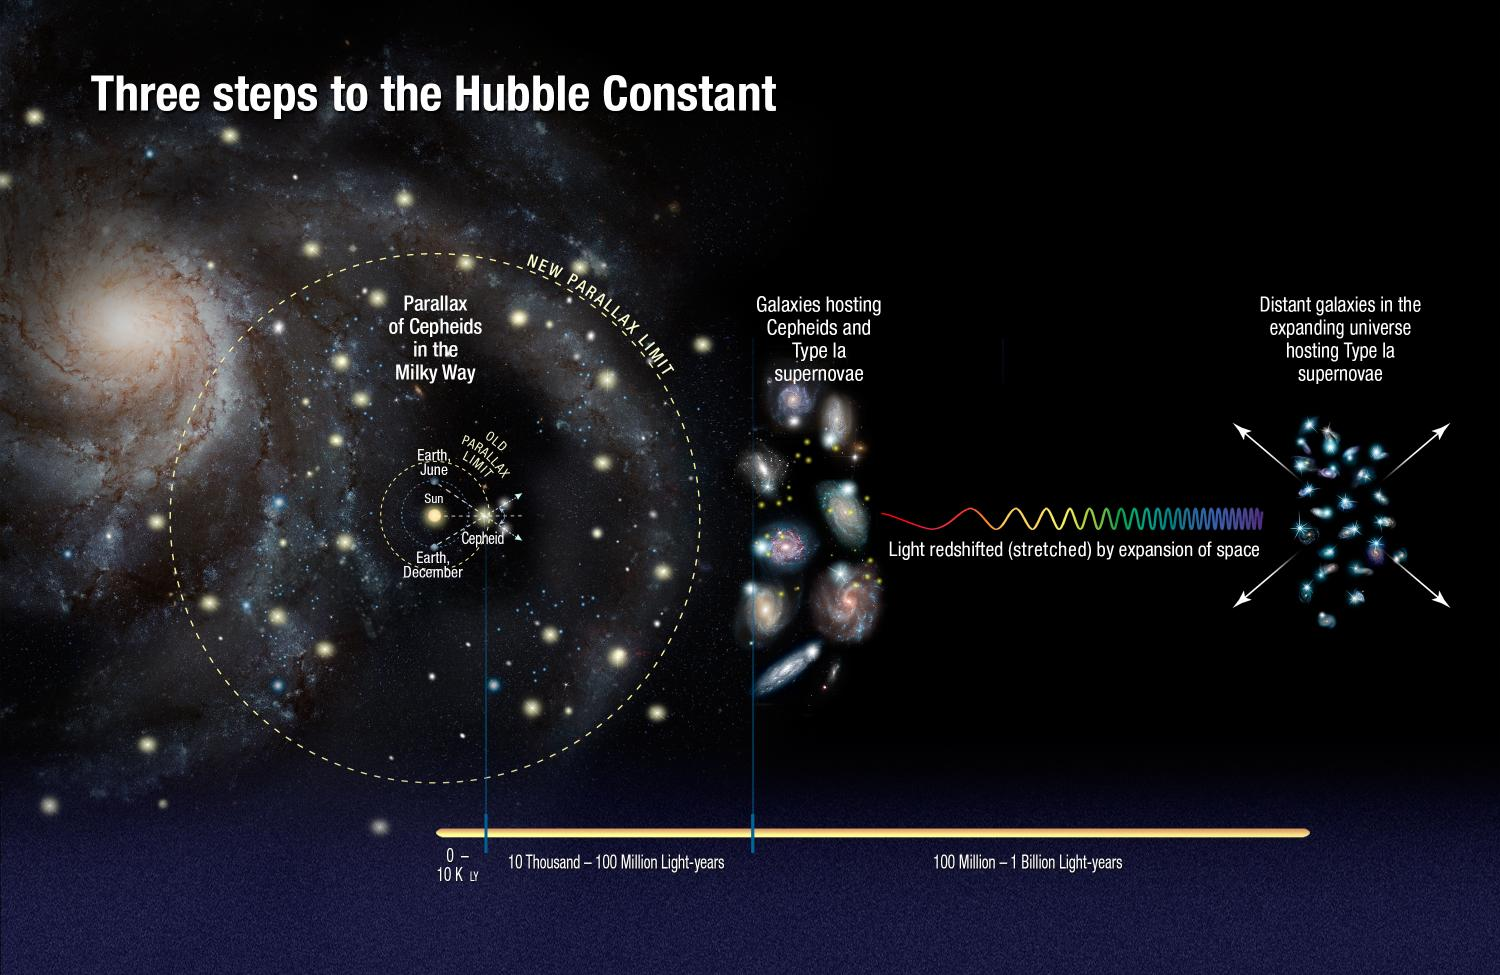
\includegraphics[width=\textwidth]{../figures/chapter-h0/hubblefindsu.jpg}}
\put(0,0){Credit:NASA}
\end{picture}
\end{figure}

\end{frame}



\begin{frame}{Where does $H_0$ enter?}
%\only<1-3>{
%\begin{figure}[hbtp]
%\centering
%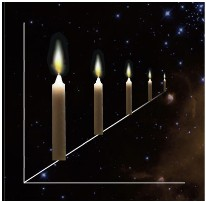
\includegraphics[scale=0.8]{../figures/chapter-h0/light-candles.jpg}
%\end{figure}}
%\only<4>{\begin{figure}[hbtp]
%\centering
%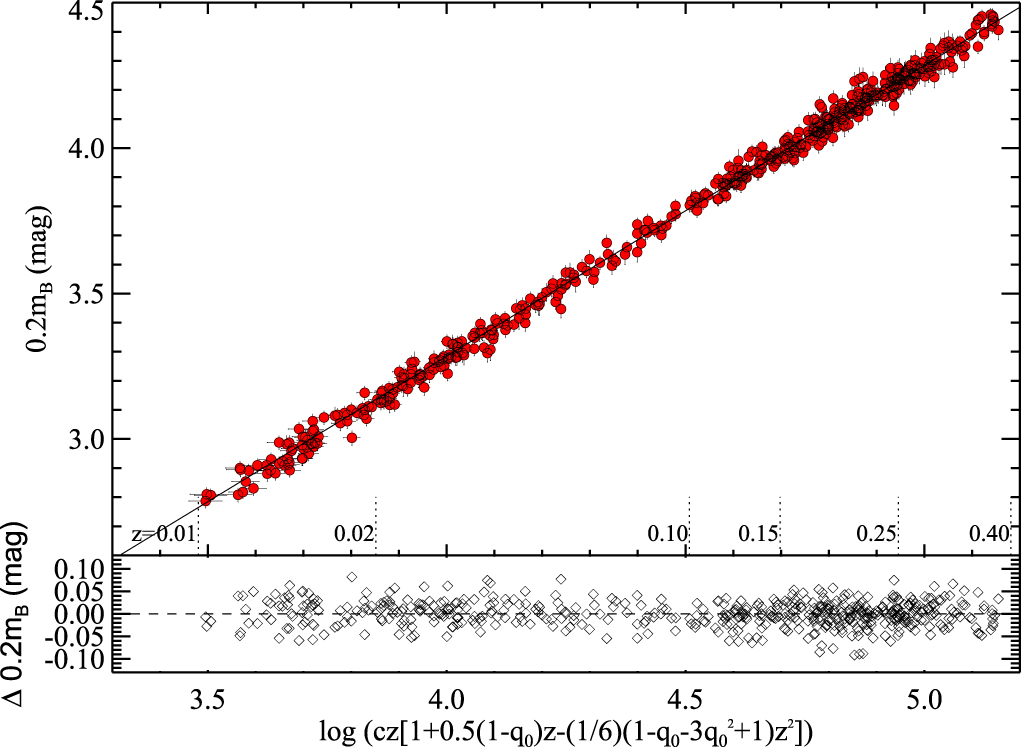
\includegraphics[scale=0.8]{../figures/chapter-h0/Hubble-diagram.jpg}
%\end{figure}}

%\begin{itemize}
%\only<1>{
%\item Estimate distances through luminosity distance
%\begin{equation*}
%d_L \equiv \left(\frac{L}{4\pi l} \right)^{1/2} \, \label{Eq:luminosity-distance-obs}
%\end{equation*}}
%\only<2-3>{
%\item Define logarithmic measures of the luminosity%: absolute and apparent magnitudes
%\only<2>{
%\begin{equation*}\label{Eq:apparent-luminosity}
%l = 10^{-2m/5}\times 2.52 \times 10^{-5}\, \mathrm{erg/ cm^2}\, \second
%\end{equation*}}
%\only<3>{
%\begin{equation*}\label{Eq:absolute-luminosity}
%L = 10^{-2M/5} \times 3.02 \times 10^{35}\, \mathrm{erg/}\second.
%\end{equation*}}}
%\only<4>{
%\item Express luminosity distance through the distance modulus
%\begin{equation*}
%\mu_0 \equiv m - M = 5 \log_{10} \left(\frac{d_L}{1 \mathrm{Mpc}} \right) + 25 \,  \label{Eq:distance-modulus}
%\end{equation*}}
\begin{itemize}
\item[] Assuming flat FLRW metric, one can compute luminosity distance
\begin{equation*}\label{Eq:luminosity-distance-the}
d_L(z) = (1+z) c \int_0^z \frac{dz'}{H(z')} \, 
\end{equation*}
%\only<2-3>{
\item[] For relatively small redshift one has
\begin{equation*}\label{Eq:luminosity-distance-the-small-z}
d_L(z) \equiv \frac{cz}{H_0}  ( 1+\delta(z)) %%\approx \frac{cz}{H_0} \left\{ 1 + \frac{1}{2} [1-q_0] z - \frac{1}{6} [1-q_0 - 3 q_0^2 + j_0] z^2 + O(z^3) \right\}
\end{equation*}
\item[] Distance modulus
\begin{equation*}
\mu_0 \equiv m - M = 5 \log_{10} \left(\frac{d_L}{1 \mathrm{Mpc}} \right) + 25 \,  \label{Eq:distance-modulus}
\end{equation*}%}
\end{itemize}
%\only<4>{
%\item 
%Determine constant $a_X$ with Supernova type Ia ($\SNe$))
%\begin{equation*}\label{Eq:av-definition}
%5 \log_{10} ( c z ( 1+\delta(z) )) - m_X = 5 \log_{10} H_0 - M_X - 25 \equiv 5 a_X \, 
%\end{equation*}}
%\end{itemize}
\end{frame}


\begin{frame}{Where does $H_0$ enter?}
\begin{equation*}\label{Eq:av-definition}
5 \log_{10} ( c z ( 1+\delta(z) )) - m_X = 5 \log_{10} H_0 - M_X - 25 \equiv 5 a_X 
\end{equation*}
%Determine constant $a_X$ with $\SNe$
\begin{figure}[hbtp]
\centering
\setlength{\unitlength}{0.1\textwidth}
\begin{picture}(10,7)
\put(1.5,2.5){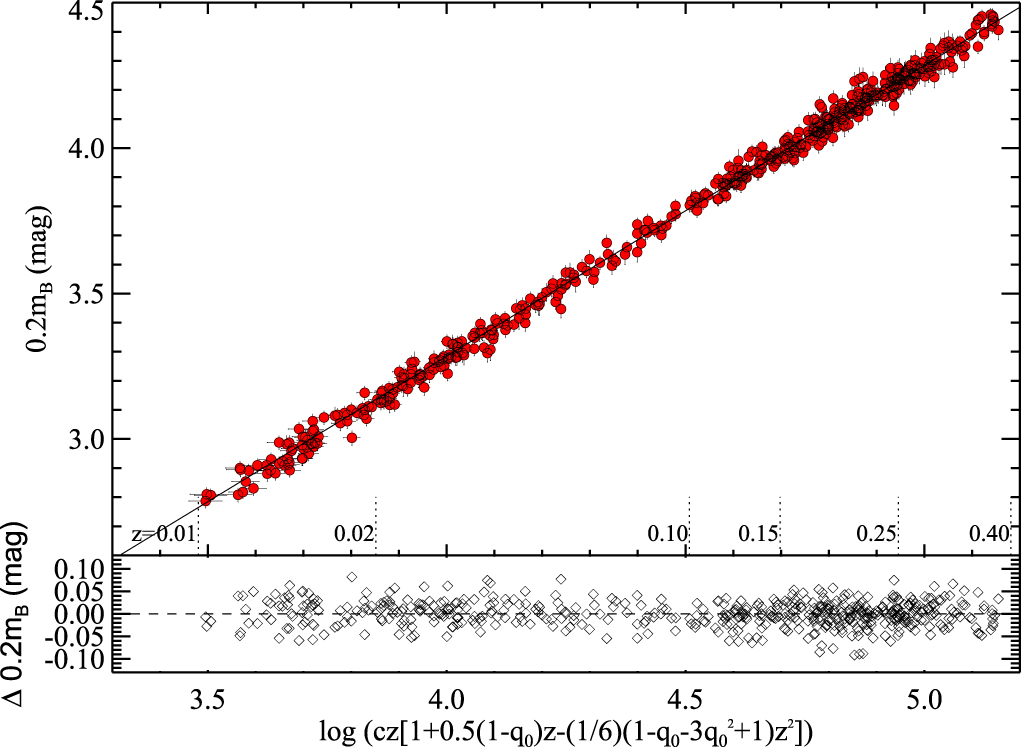
\includegraphics[scale=0.8]{../figures/chapter-h0/Hubble-diagram.jpg}}
\put(1.5,2){Credit:Riess et al. 2016}
\end{picture}
\end{figure}


\end{frame}

\begin{frame}{Modelling Cepheids and $\SNe$ apparent magnitudes}
\begin{itemize}
\item $\SNe$ apparent magnitudes
\begin{equation*}
m_{X,i}^{\SNe} =  5 \log_{10} H_0 + \mu_{0,i} - 5 a_X - 25 \, %. \label{Eq:apparent-magnitude-H0}
\end{equation*}
\item Cepheid variables apparent magnitudes 
\begin{equation*}\label{Eq:P-L-equation}
m_{Y,i,j}^{\Cepheid} = \mu_{0,i} + M_Y^{\Cepheid} + b_Y (\log P_{i,j}-1) + Z_Y \Delta \log[O/H]_{i,j}%,
\end{equation*}
%\item Galaxies hosting both $\SNe$ and Cepheid stars
%\item A few anchor distances: $\mu_0^\LMC$, $\mu_0^\NGC$, $\mu_0^\MAnd$, $\MW$ Cepheid stars parallaxes 
\end{itemize}
\end{frame}

\begin{frame}{Summarising, to measure $H_0$ you have to:}
\begin{enumerate}
\item Calibrate distance ladder with geometrical distance estimates (e.g., Milky Way Cepheids, $\NGC$, $\LMC$, $\MAnd$)
\item Find galaxies simultaneously hosting $\SNe$ and Cepheid stars
\item Use distant $\SNe$ to calibrate low redshift $\SNe$ and find $H_0$ through a global fit of Cepheid and $\SNe$ apparent magnitudes:
\item[]
\begin{equation*}
m_{X,i}^{\SNe} =  5 \log_{10} H_0 + \mu_{0,i} - 5 a_X - 25 \, %. \label{Eq:apparent-magnitude-H0}
\end{equation*}
\begin{equation*}\label{Eq:P-L-equation}
m_{Y,i,j}^{\Cepheid} = \mu_{0,i} + M_Y^{\Cepheid} + b_Y (\log P_{i,j}-1) + Z_Y \Delta \log[O/H]_{i,j}%,
\end{equation*}
\end{enumerate}
\end{frame}

\begin{frame}{Weak points in current analyses: Riess et al. and G. Efstathiou}
\begin{itemize}
\item Need to determine $H_0$, but \textbf{data sets include outliers}...
\item Riess et al. and G. Efstathiou used standard $\chi^2$ minimisation and \textbf{outlier rejection algorithms} to deal with outliers
\item G. Efstathiou used a \textbf{period cut-off} of $60$ days in the period luminosity relation. Riess et al. did not use period cut-off
\item G. Efstathiou did not use neither Milky Cepheid stars nor direct measurement to the LMC as \textbf{anchor distances}
\item \textbf{Discarding data involves arbitrary choices} (e.g., Chauvenet's criterion) and might hinder understanding of data sets
\item Can we do better? 
\end{itemize}
\end{frame}

\begin{frame}{$\chi^2$ analysis including outliers may bias constraints}
\begin{figure}[hbtp]
\centering
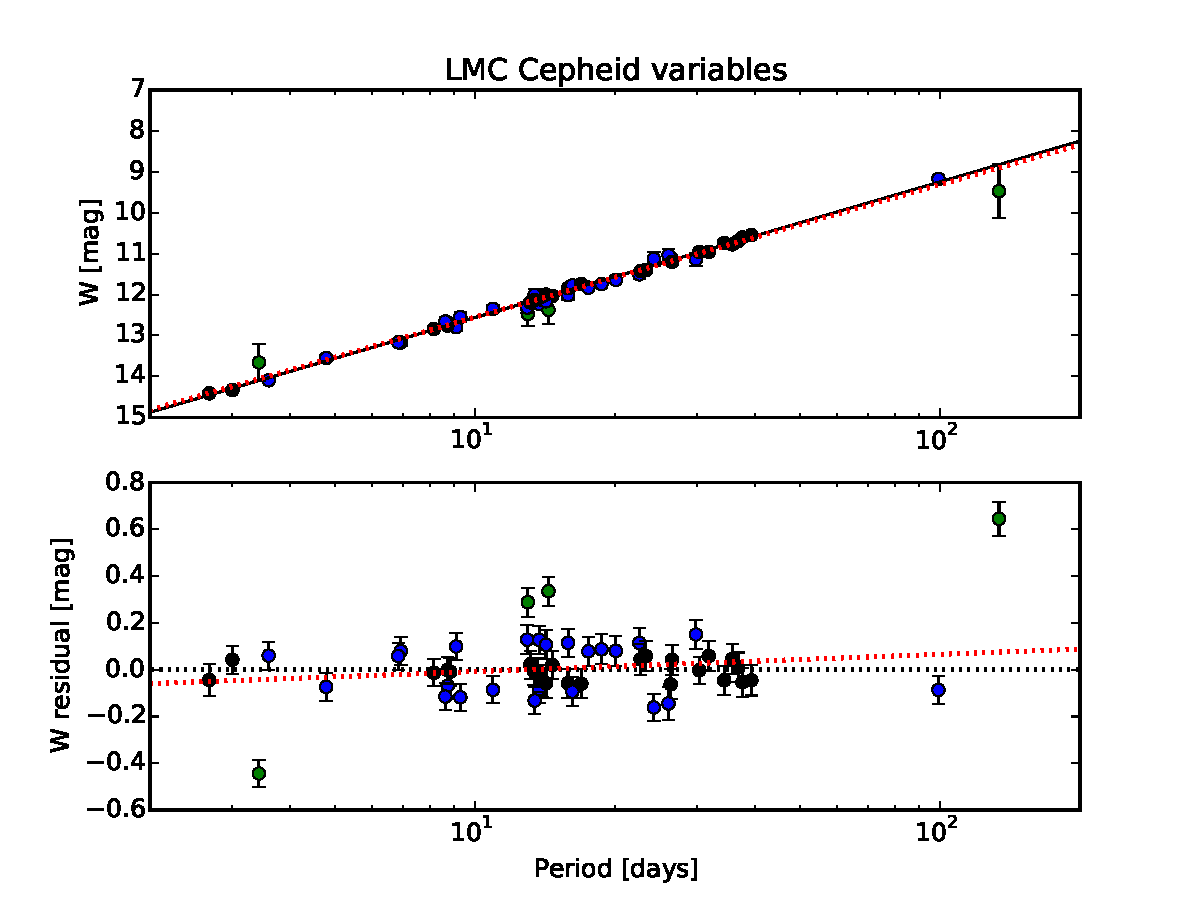
\includegraphics[width=0.95\textwidth]{effective_HP_cepheids_LMC.pdf}
\end{figure}
\end{frame}

\setbeamercolor{frametitle}{bg=orange}

\section{Determining $H_0$ with Bayesian hyper-parameters}

\begin{frame}{Our method to determine $H_0$}

\begin{itemize}
\item It is usually assumed that data points are drawn from a Gaussian PDF
\begin{equation*}
P_G(D_i|\vec{w}) = \tilde{N}_i \, \frac{\exp(-\chi^2_i(\vec{w})/2)}{\sqrt{2\pi}}
\end{equation*}
\item We drop this assumption and consider error bars could have been underestimated. Hyper-parameters (HP) can rescale error bars (if needed) 
\begin{equation*}
\sigma_i \rightarrow \sigma_i/\sqrt{\alpha_i}
\end{equation*}
\end{itemize}
\end{frame}

\begin{frame}{Our method to determine $H_0$}
\only<3>{
\begin{figure}[hbtp]
\centering
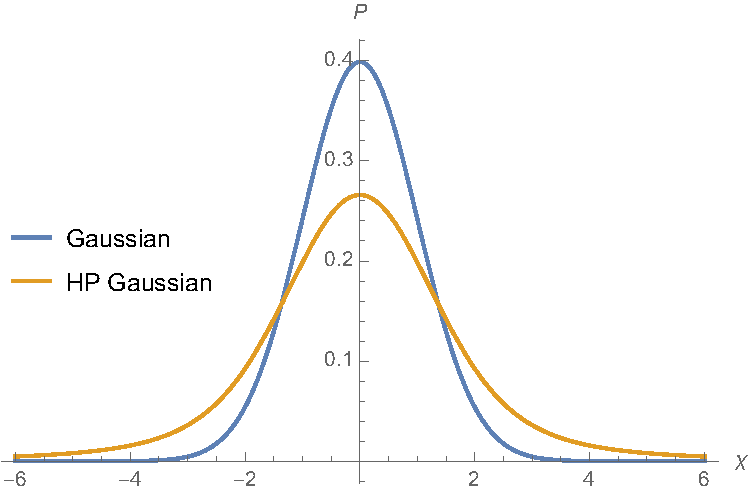
\includegraphics[scale=0.7]{../figures/chapter-h0/PDF.pdf}
\end{figure}
}
\begin{itemize}
\only<1-2>{
\item We start from a Gaussian PDF with usual $\chi^2$, but allow error bars to become greater $\alpha_i \in [0,1]$ and take into account every possible value for the rescaling (marginalise over HPs)
\item We obtain a new PDF: a Gaussian HP PDF 
\begin{equation*}
P(D_i|\vec{w}\,) = \tilde{N}_i \, \left(\frac{ \mathrm{Erf}\left( \frac{\chi_i(\vec{w})}{\sqrt{2}} \right)  -\sqrt{\frac{2}\pi} \chi_i(\vec{w}) \exp(-\chi^2_i(\vec{w})/2)}{ \chi^3_i(\vec{w})} \right)
\end{equation*}}
\item[]
\end{itemize}
\end{frame}

\begin{frame}{Our method to determine $H_0$}
\begin{itemize}
\item Next, we maximise the likelihood and compute effective HPs for each datum (given the best fitting parameters)
\begin{eqnarray*}
\alpha^{\eff}_i & = 1,\quad \mathrm{if} \quad \chi^2_i\leq1
\\
\alpha^{\eff}_i & = \frac{1}{\chi^2_i},\quad \mathrm{if} \quad \chi^2_i> 1
\end{eqnarray*}
\item Finally, we asses the compatibility of the data sets through normalised weights
\begin{equation*}
|| \alpha^{j} || \equiv \frac{\sum_{i=1}^{K_j} \alpha_{i,j}}{K_j}
\label{Eq:normalised-weights}
\end{equation*}
$j=\Cepheid,\,\SNe,\,\Anchors$\\
$K_j$: number of data points of kind $j$ 
\end{itemize}

\end{frame}

\begin{frame}{Our method to determine $H_0$ in practice}
\begin{enumerate}
\item The data points are drawn from a HP Gaussian PDF
\item We do a simultaneous fit to Cepheid stars and $\SNe$
\item This allows you to obtain the best-fitting parameters for the model and compute effective HPs for each  datum
\item Using normalised  weights helps to asses the compatibility of all kinds of data sets  
\end{enumerate}
\end{frame}

\begin{frame}{Applying hyper-parameters to data}
\begin{enumerate}
\item The R11 data set: $8$ galaxies simultaneously hosting $\SNe$ and Cepheid stars, three anchor distances ($\mu_0^\LMC$, $\mu_0^\NGC$, 13 $\MW$ Cepheid stars parallaxes)
\item The R16 data set: $19$ galaxies simultaneously hosting $\SNe$ and Cepheid stars, four anchor distances ($\mu_0^\LMC$, $\mu_0^\NGC$, $\mu_0^\MAnd$, 15 $\MW$ Cepheid stars parallaxes)
\end{enumerate}
\end{frame}

\setbeamercolor{frametitle}{bg=dodger}
\begin{frame}{Results: the R11 data set: No reasons to discard data}

G. Efstathiou excluded both MW parallaxes and direct distance to LMC as anchor distances

\begin{table}[tbp]
\centering
\begin{tabular}{@{}ccccc}
\hline
\multicolumn{5}{c}{Consistency of period-luminosity relation} \\
\hline
Fit & Galaxy & $M_W$ & $b_W$ & $\sigma_{\intt}$ \\
\hline
 c & $\LMC$ & $-5.93\,(0.07)$& $-3.31\,(0.05)$& $0.06$  \\
 
 e & $\MW$ & $-5.88\,(0.07)$ & $-3.30\,(0.26)$ & $0.02$  \\
  
 f & $\NGC$ & $-6.12\,(0.15)$&$-3.02\,(0.17)$ & $0.12$  \\

\hline
\end{tabular}
\end{table}
We found no reasons to exclude data sets: period-luminosity relation compatible with direct distance determinations
\end{frame}

\begin{frame}{Uncertainty of $H_0$ depends on number of HP}
\begin{center}
%\item[]
\only<1>{Standard $\chi^2$ analysis with outlier rejection algorithm}
\only<2>{HPs in Cepheid stars}
\only<3>{HPs in Cepheid stars and anchor distances}
\only<4>{HPs in Cepheid stars and $\SNe$}
\only<5>{HPs in Cepheid stars, anchor distances and $\SNe$}
\only<6>{$H_0 = 75.0 \pm 3.9 \, \km\, \second^{-1}\, \Mpc^{-1}$ }
\only<7>{$|| \alpha^{\Cepheid}|| = 0.72 $, $|| \alpha^{\SNe}|| = 0.74$, $|| \alpha^{\Anchors}|| = 0.86$}
\end{center}

\begin{figure}
\centering
\only<1>{
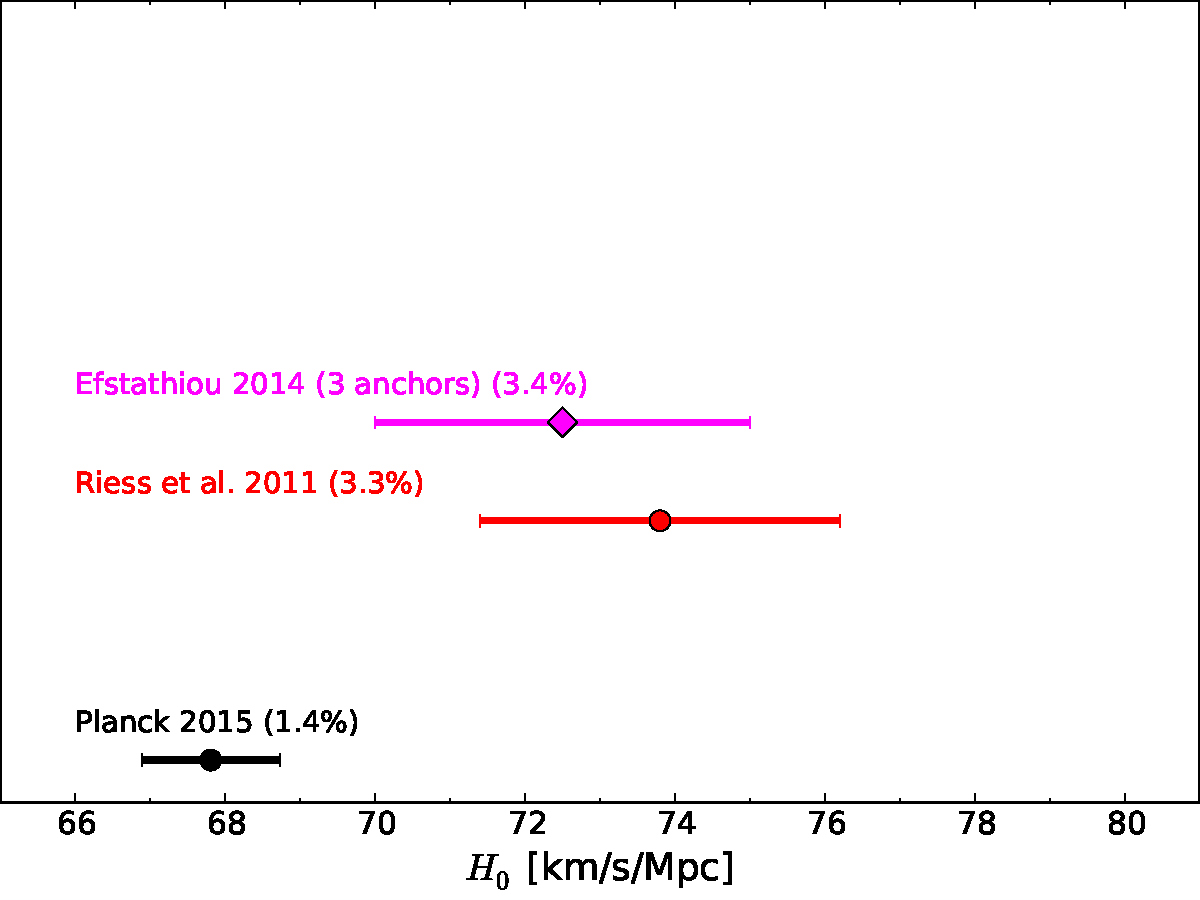
\includegraphics[scale=0.4]{../figures/chapter-h0/H0_values_three_anchors-1.pdf}} 
\only<2>{
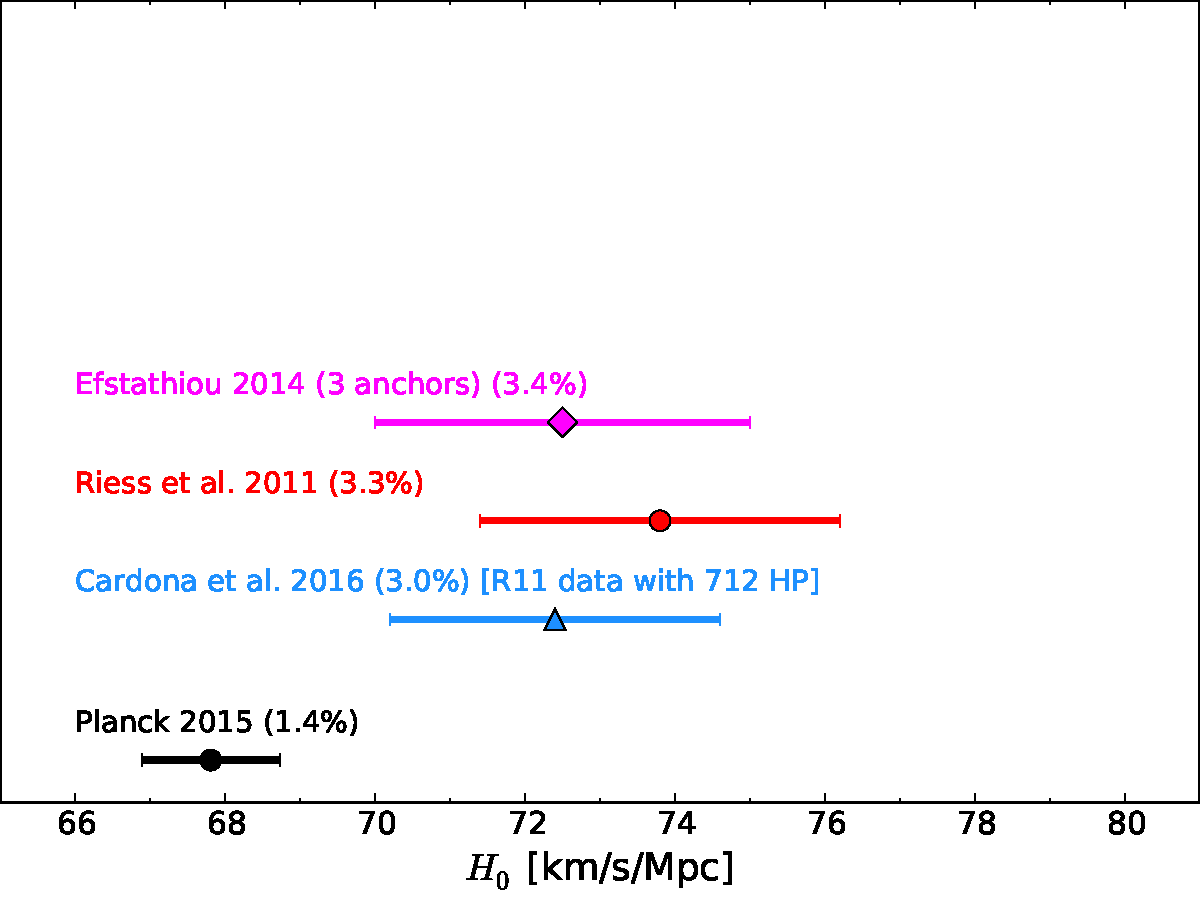
\includegraphics[scale=0.4]{../figures/chapter-h0/H0_values_three_anchors-2.pdf}}
\only<3>{
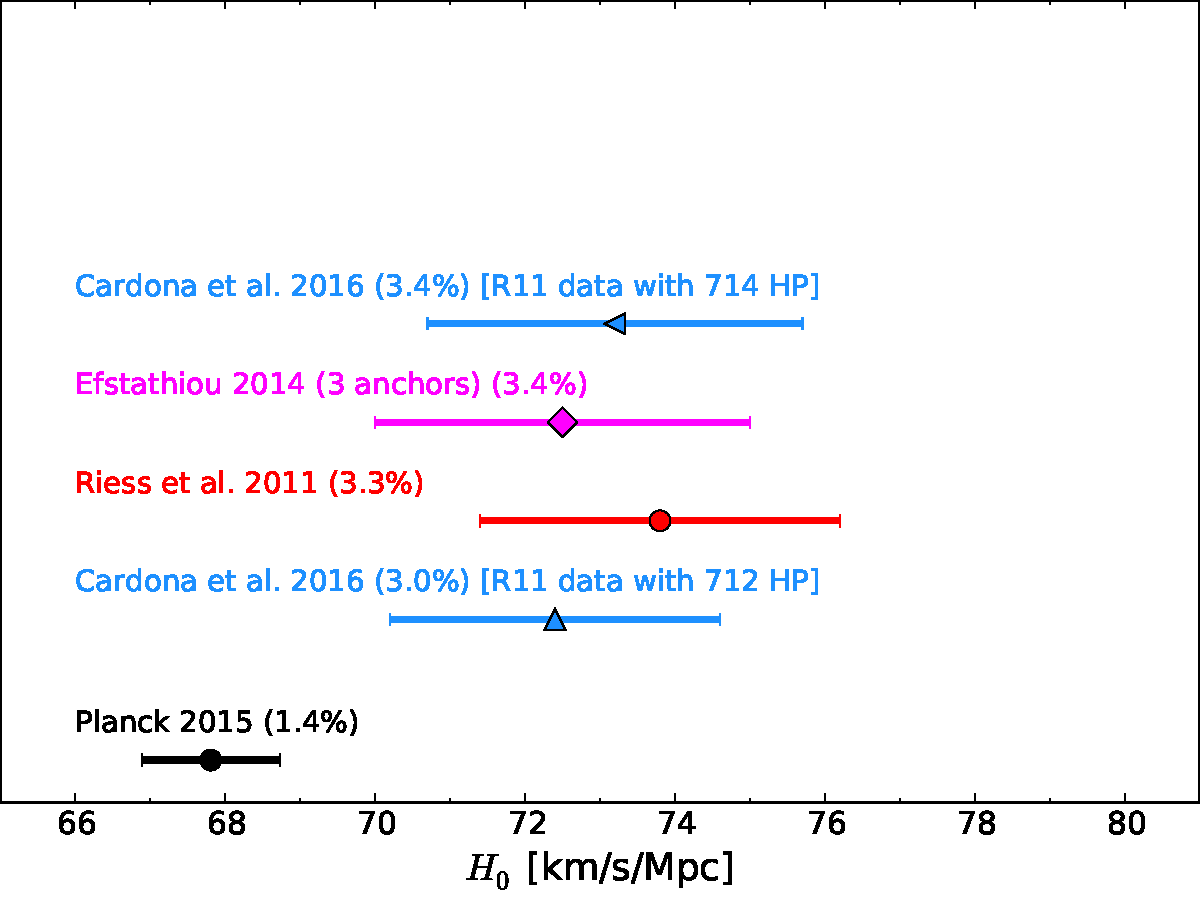
\includegraphics[scale=0.4]{../figures/chapter-h0/H0_values_three_anchors-3.pdf}}
\only<4>{
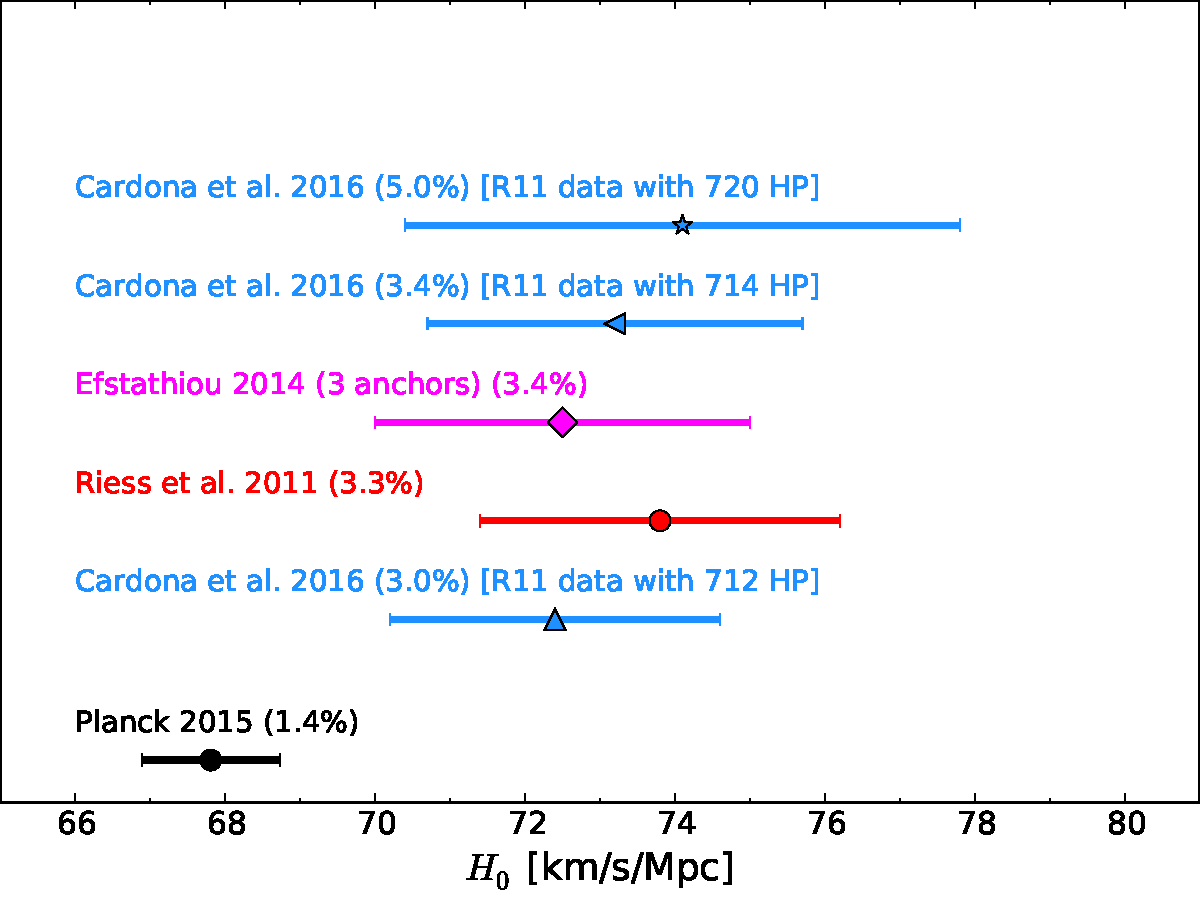
\includegraphics[scale=0.4]{../figures/chapter-h0/H0_values_three_anchors-4.pdf}}
\only<5-7>{
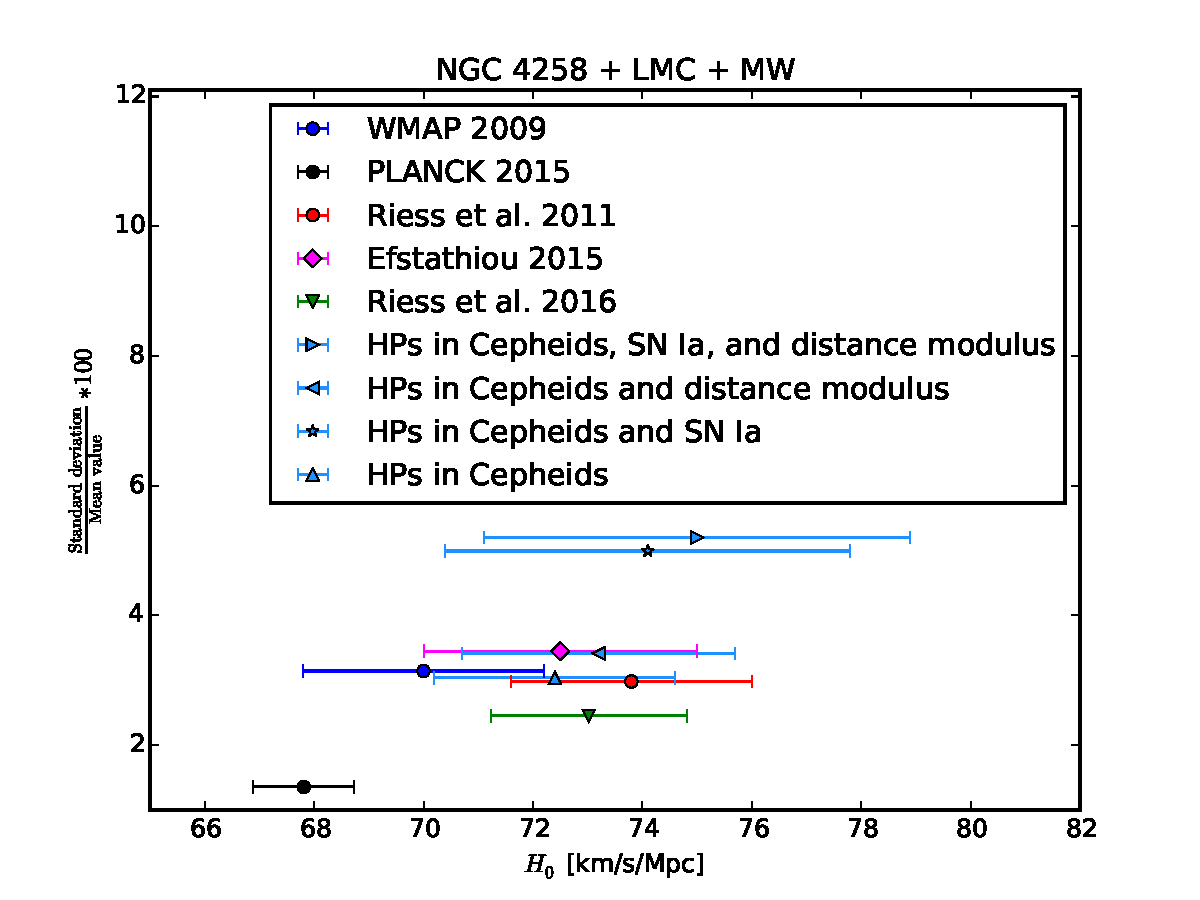
\includegraphics[scale=0.4]{../figures/chapter-h0/H0_values_three_anchors.pdf}}
\end{figure}
\end{frame}

%\begin{frame}{Baseline result for the R11 data set}
%
%\begin{equation*}
%	H_0 = 75.0 \pm 3.9 \, \mathrm{km/s/Mpc}  
%\end{equation*}
%
%\begin{equation*}
%	|| \alpha^{\Cepheid}|| = 0.72  
%\end{equation*}
%
%\begin{equation*}
%	|| \alpha^{\SNe}|| = 0.74   
%\end{equation*}
%
%\begin{equation*}
%	|| \alpha^{\Anchors}|| = 0.86 
%\end{equation*}
%
%\begin{equation*}
%	\sum_j ||\alpha^j|| = 2.32  
%\end{equation*}
%
%\end{frame}

\begin{frame}{$28\%$ Cepheid stars effectively down-weighted}
\begin{center}
Normalised weight in Cepheid sample: $|| \alpha^{\Cepheid}|| = 0.72$
\end{center}
\begin{figure}
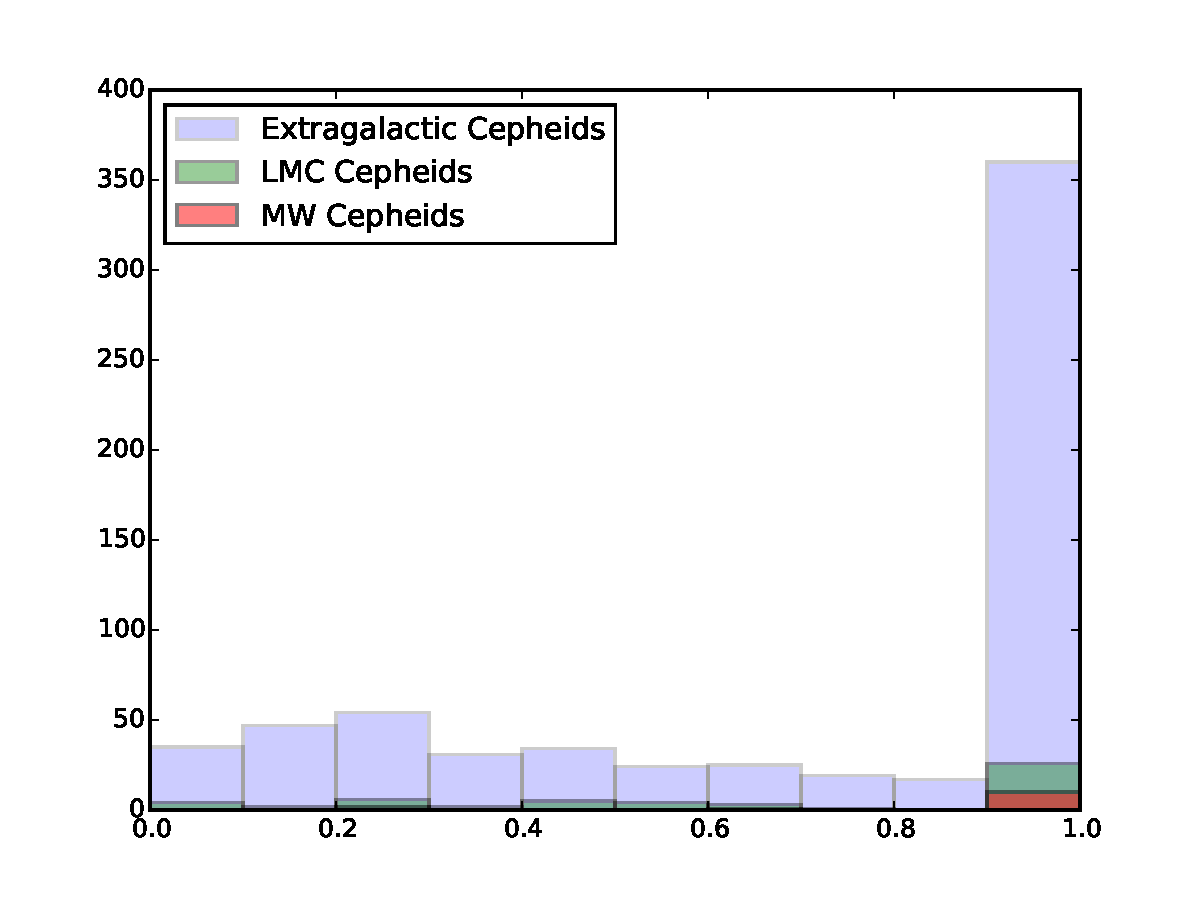
\includegraphics[scale=0.4]{../figures/chapter-h0/effective_HP_histogram.pdf} 
\end{figure}
\end{frame}

\begin{frame}{Inconsistencies in $\SNe$ data}
\begin{center}
Normalised weight in $\SNe$ data: $|| \alpha^{\SNe}|| = 0.74 $
\end{center}
\begin{figure}
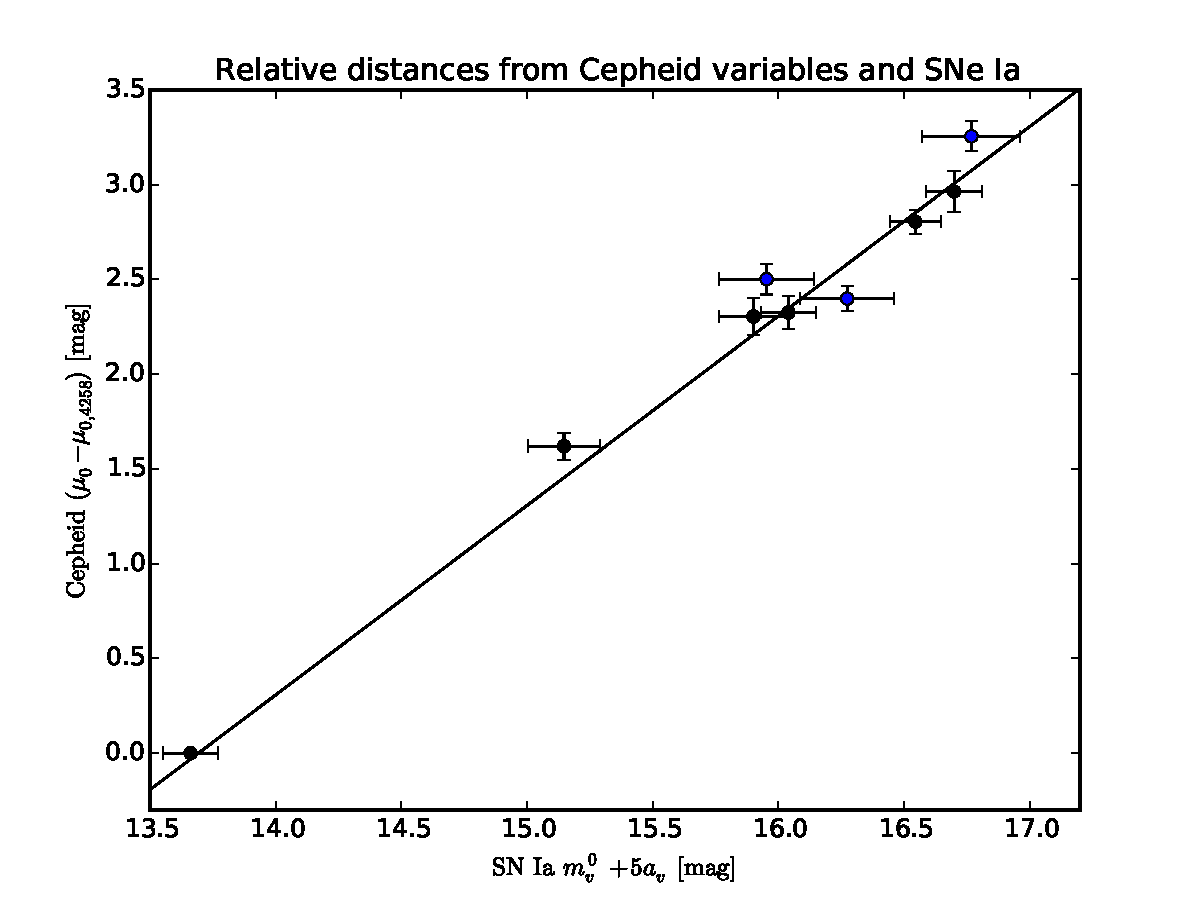
\includegraphics[scale=0.45]{../figures/chapter-h0/effective_HP_SNIa.pdf} 
\end{figure}
\end{frame}

\begin{frame}{Anchor choice plays a part in the analysis}
\begin{figure}
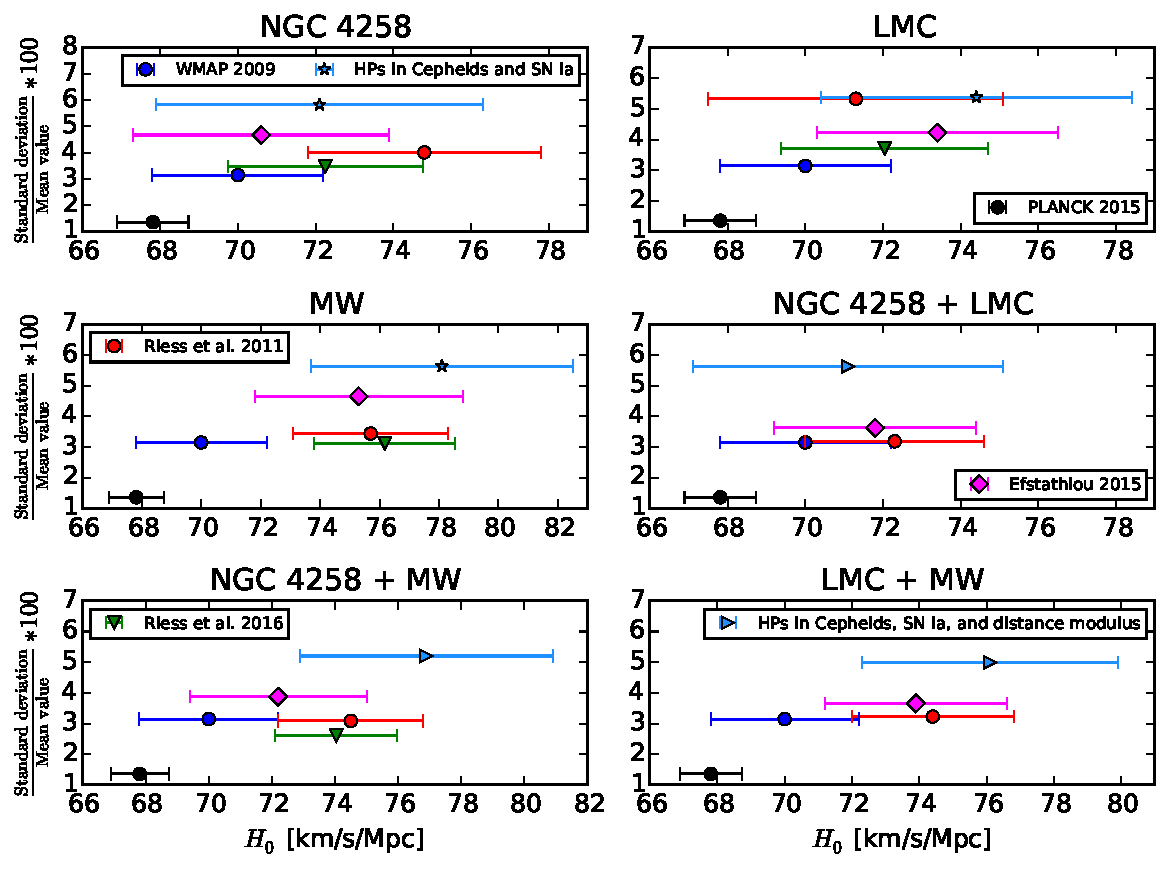
\includegraphics[scale=0.5]{../figures/chapter-h0/H0_values_anchor_combination.pdf} 
\end{figure}
\end{frame}

\setbeamercolor{frametitle}{bg=aquamarine}

\begin{frame}{Baseline result for the R16 data set}
\begin{itemize}
\item[] Considered variants of baseline analysis (e.g., period cut-off, metallicity dependence, reddening law) and computed systematic error due to these changes 
\begin{equation*}
\sigma_{\rm syst}=0.20 \km\, \second^{-1}\, \Mpc^{-1} 
\end{equation*}
\item[] Baseline result for the R16 data set
\begin{equation*}
H_0 = 73.75 \pm 2.11\,\km\, \second^{-1}\, \Mpc^{-1}
\end{equation*}
\end{itemize}
\end{frame}

\begin{frame}{Comparing compatibility in R11 and R16 data sets}
\begin{itemize}
\item Riess et al. 2011 rejects about $20\%$ of Cepheids (outliers were released)
\item Riess et al. 2016 rejects about $2\%$ of Cepheids (outliers were not released)
\end{itemize}
\begin{table}[tbp]
\centering
\begin{tabular}{@{}ccccc}
\hline
\multicolumn{4}{c}{Consistency of different kinds of data} \\
\hline
Data set &$|| \alpha^{\Cepheid}||$ & $|| \alpha^{\SNe}||$ & $|| \alpha^{\Anchors}||$ \\
\hline
 R11 &  $ 0.72 $ & $ 0.74 $ & $0.86$  \\
 
 R16 &  $ 0.86 $ & $ 0.78 $ & $0.92$  \\
  
% f & $\NGC$ & $-6.12\,(0.15)$&$-3.02\,(0.17)$ & $0.12$  \\

\hline
\end{tabular}
\end{table}
\end{frame}

\begin{frame}{Comparison of our two baselines fits}
\begin{figure}
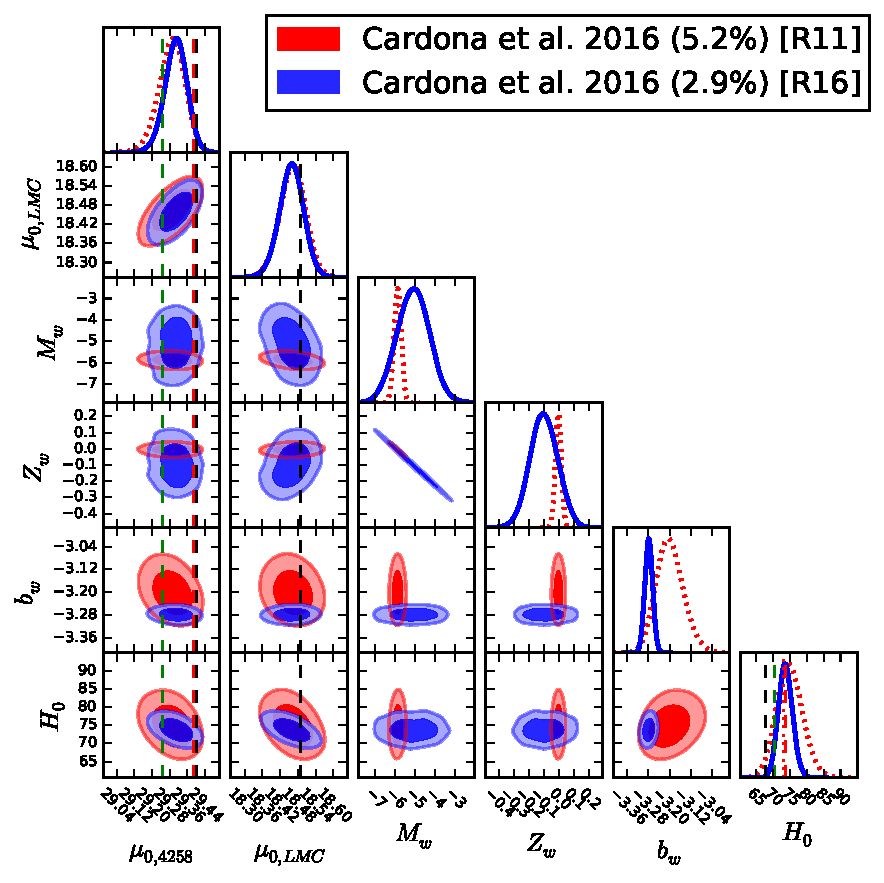
\includegraphics[scale=0.5]{../figures/chapter-h0/triangle_plot_fit_29_44.pdf} 
\end{figure}
\end{frame}

\begin{frame}{$14\%$ Cepheid stars effectively down-weighted}
\begin{center}
Normalised weight in the Cepheid sample: $|| \alpha^{\Cepheid}|| = 0.86$
\end{center}
\begin{figure}
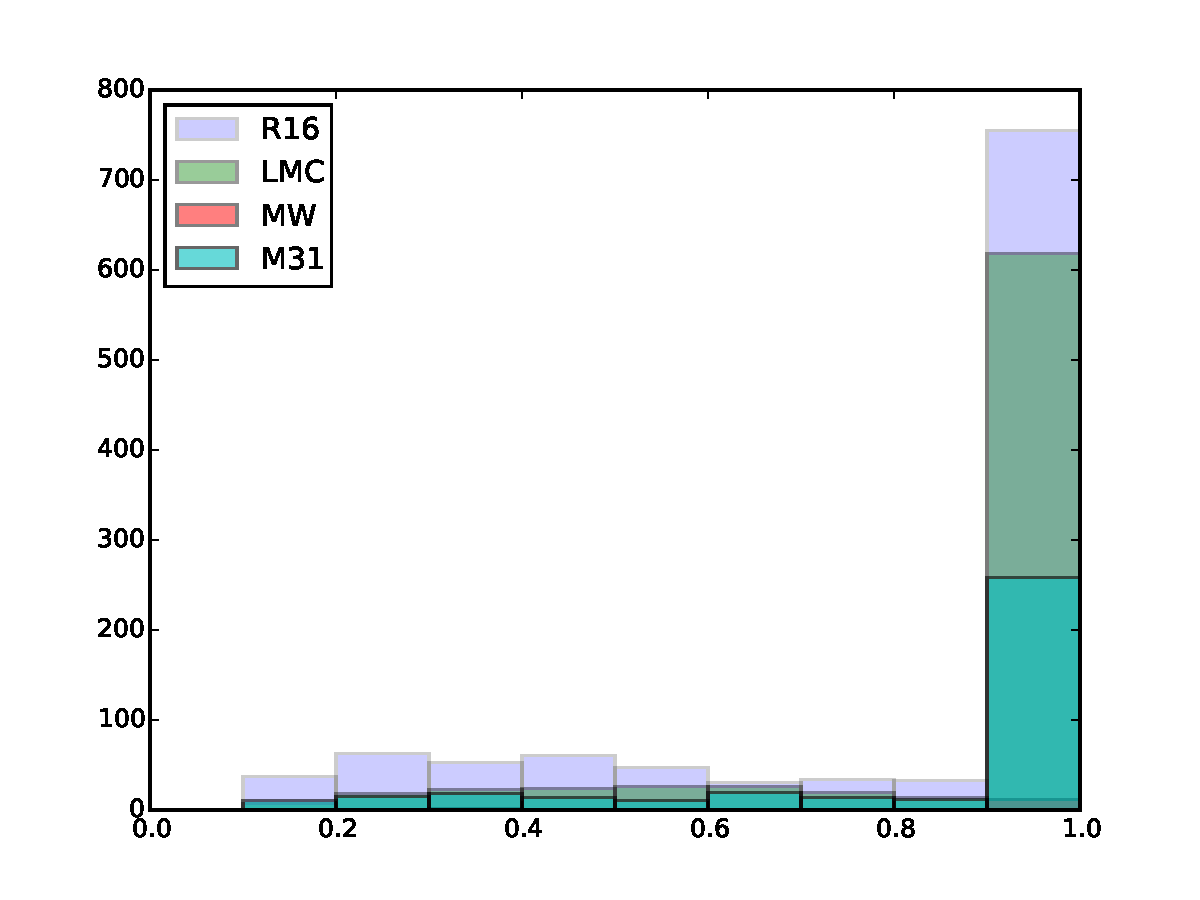
\includegraphics[scale=0.4]{../figures/chapter-h0/effective_HP_histogram_R16.pdf} 
\end{figure}
\end{frame}

\begin{frame}{Inconsistencies in $\SNe$ data}
\begin{center}
Normalised weight in $\SNe$ data: $|| \alpha^{\SNe}|| = 0.78 $
\end{center}
\begin{figure}
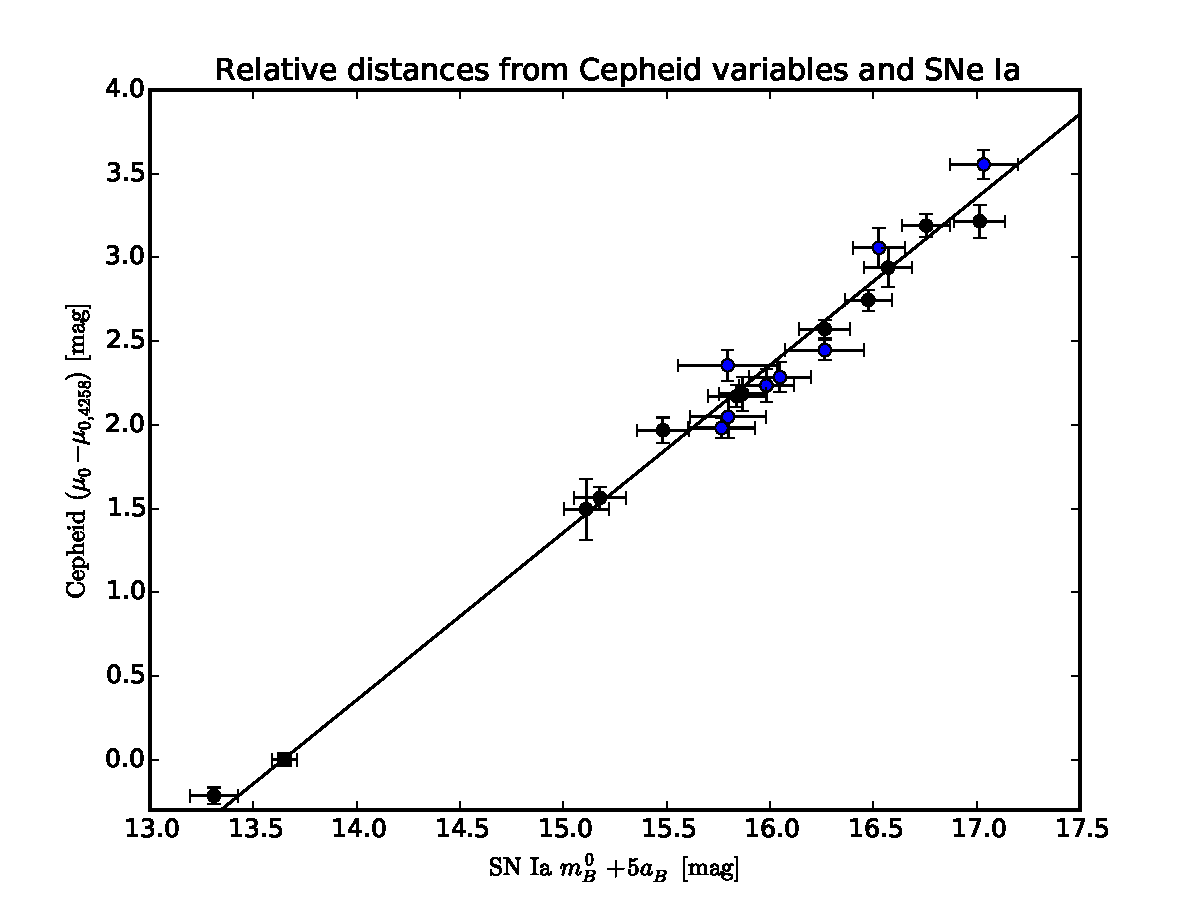
\includegraphics[scale=0.45]{../figures/chapter-h0/effective_HP_SNIa_R16.pdf} 
\end{figure}
\end{frame}



\begin{frame}{$3.1\sigma$ tension between direct and inferred $H_0$}
\begin{figure}
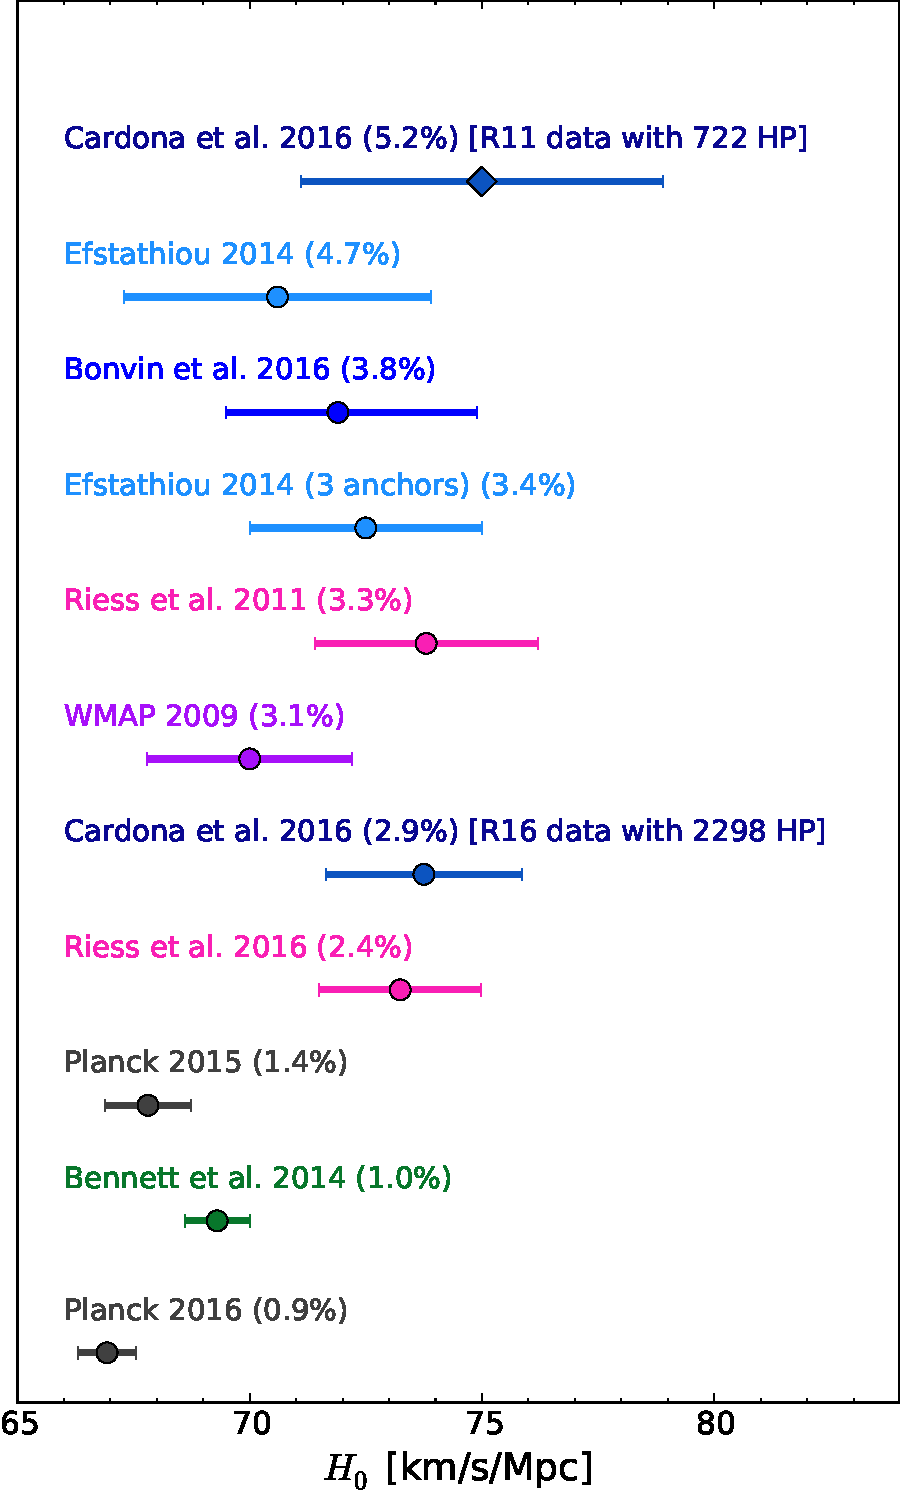
\includegraphics[scale=0.3]{../figures/chapter-h0/H0_best_estimates.pdf} 
\end{figure}
\end{frame}

\setbeamercolor{frametitle}{bg=orange}

\section{Takeaways}

\begin{frame}{Takeaways}
\begin{itemize}
%\item Developed a method to search for deviations of statistical isotropy: CMB data from Planck is consistent with the Cosmological principle. 
%\item Data is consistent with zero dark energy anisotropic stress
%\item Lensing convergence must be included in analyses of upcoming galaxy surveys

\item Developed a method to measure the Hubble constant and asses consistency of data sets
\item Hyper-parameter analysis avoids the use of arbitrary outlier rejection algorithms
\item Anchor distances play a part in the determination of $H_0$. We did not find evident reasons to discard any of them. 
\item Confirmed ($3.1\sigma$) tension between CMB and local measurements of $H_0$. This might suggest new physics or unaccounted systematics in the data sets
\item Universe appears to expand faster ($9$-$10\%$) than predicted by the  concordance model of cosmology. If not an error, it could be key to understand $95\%$ of the Universe
%\item New measurements of Milky Way Cepheid stars by Gaia (2022) will be important to improve the distance ladder and therefore reduce uncertainty of $H_0$.    
\end{itemize}
\end{frame}

\setbeamercolor{frametitle}{bg=dodger}

\section*{Project 1: testing statistical isotropy with Planck data}

\begin{frame}{CMB anisotropies}
\begin{figure}[hbtp]
\centering
\only<1,5>{
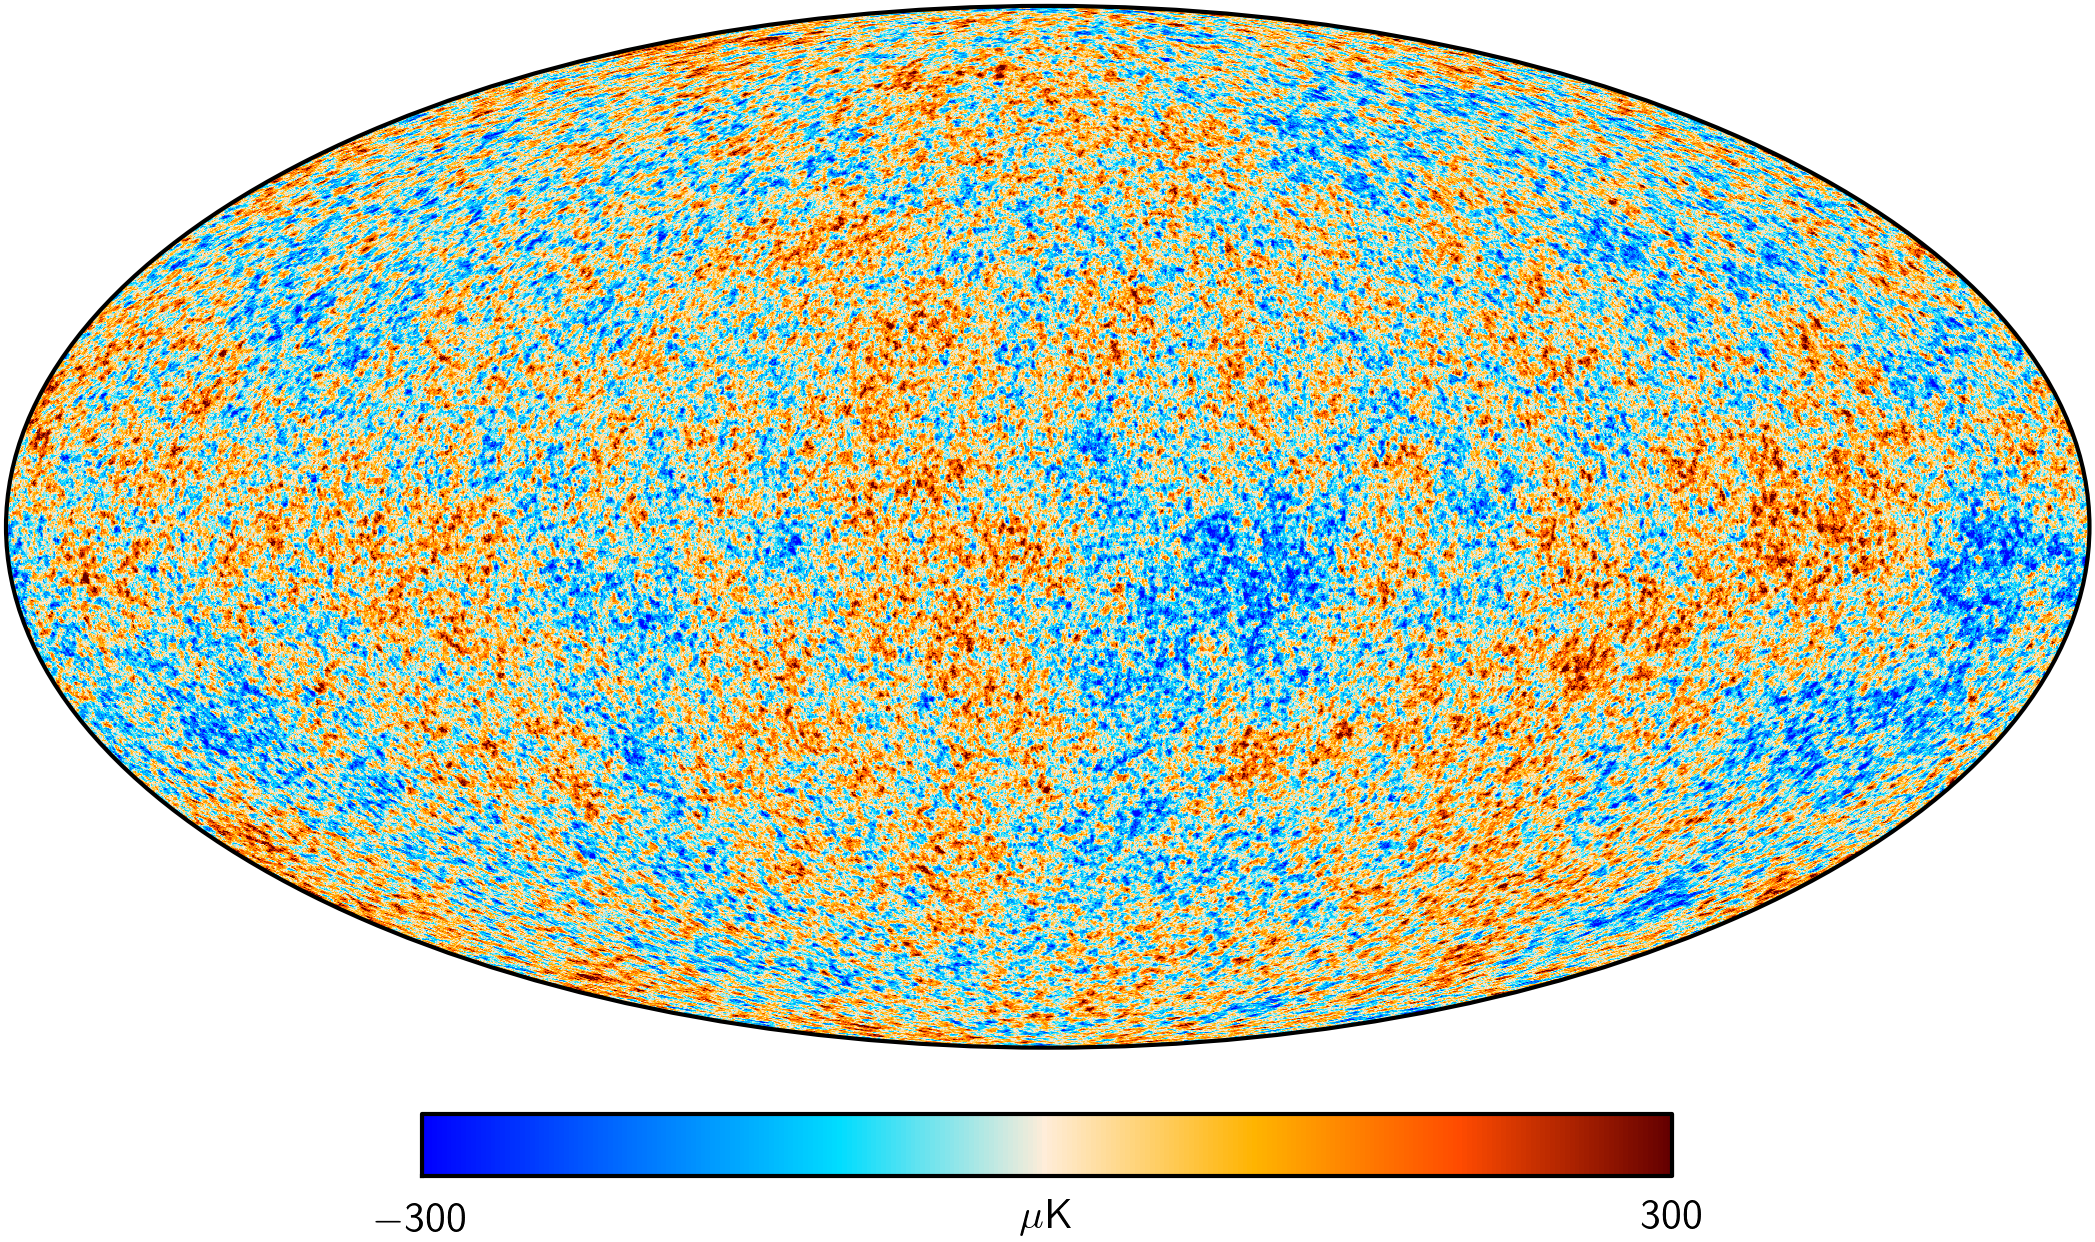
\includegraphics[width=\textwidth]{../figures/2015_SMICA_CMB.png}}
\only<2>{
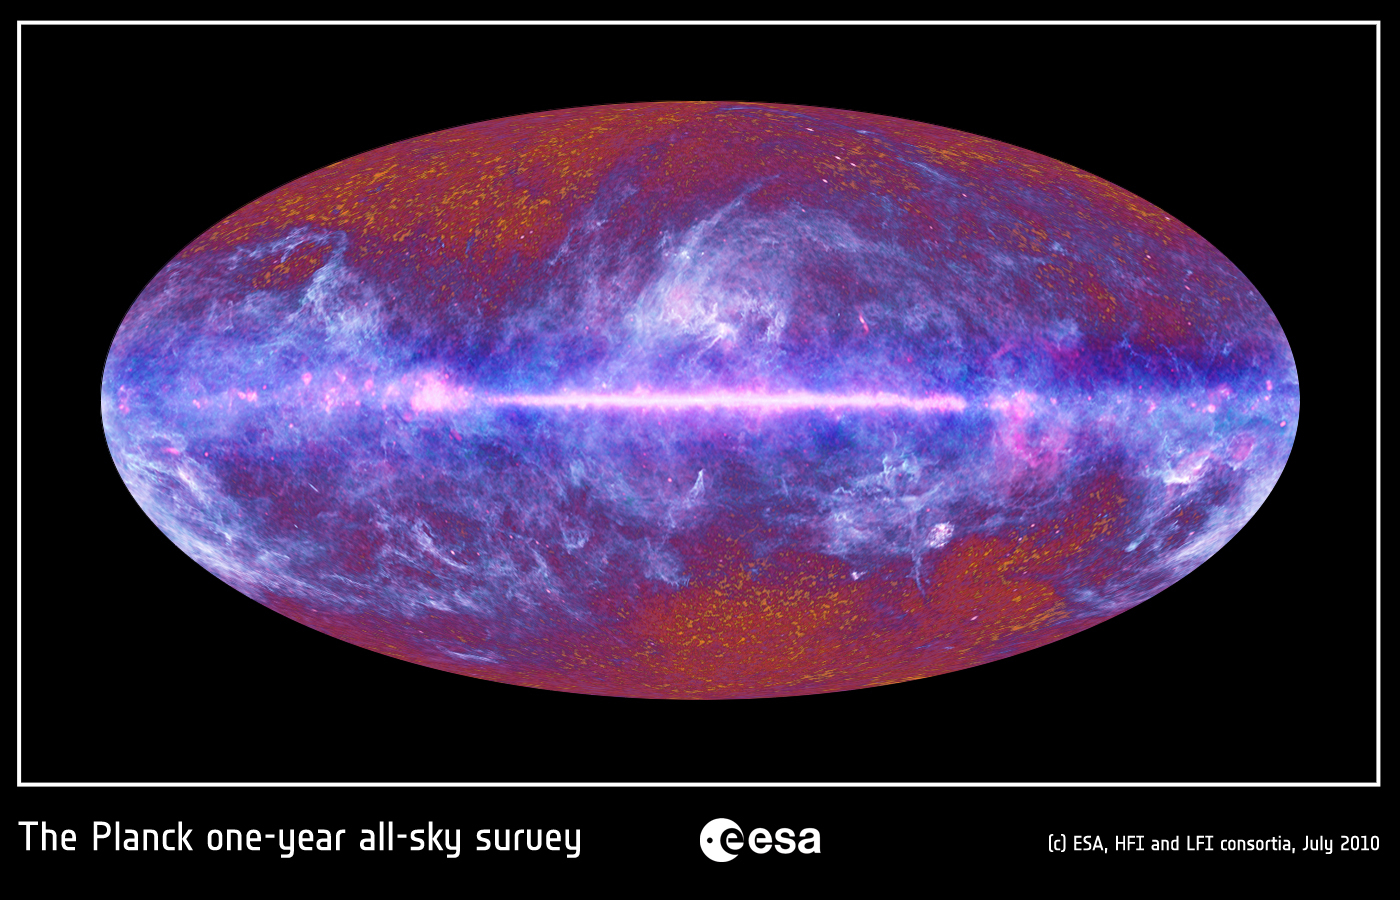
\includegraphics[width=0.9\textwidth]{../figures/PLANCK_FSM_03_Black_frame_orig.jpg}}
\only<3>{
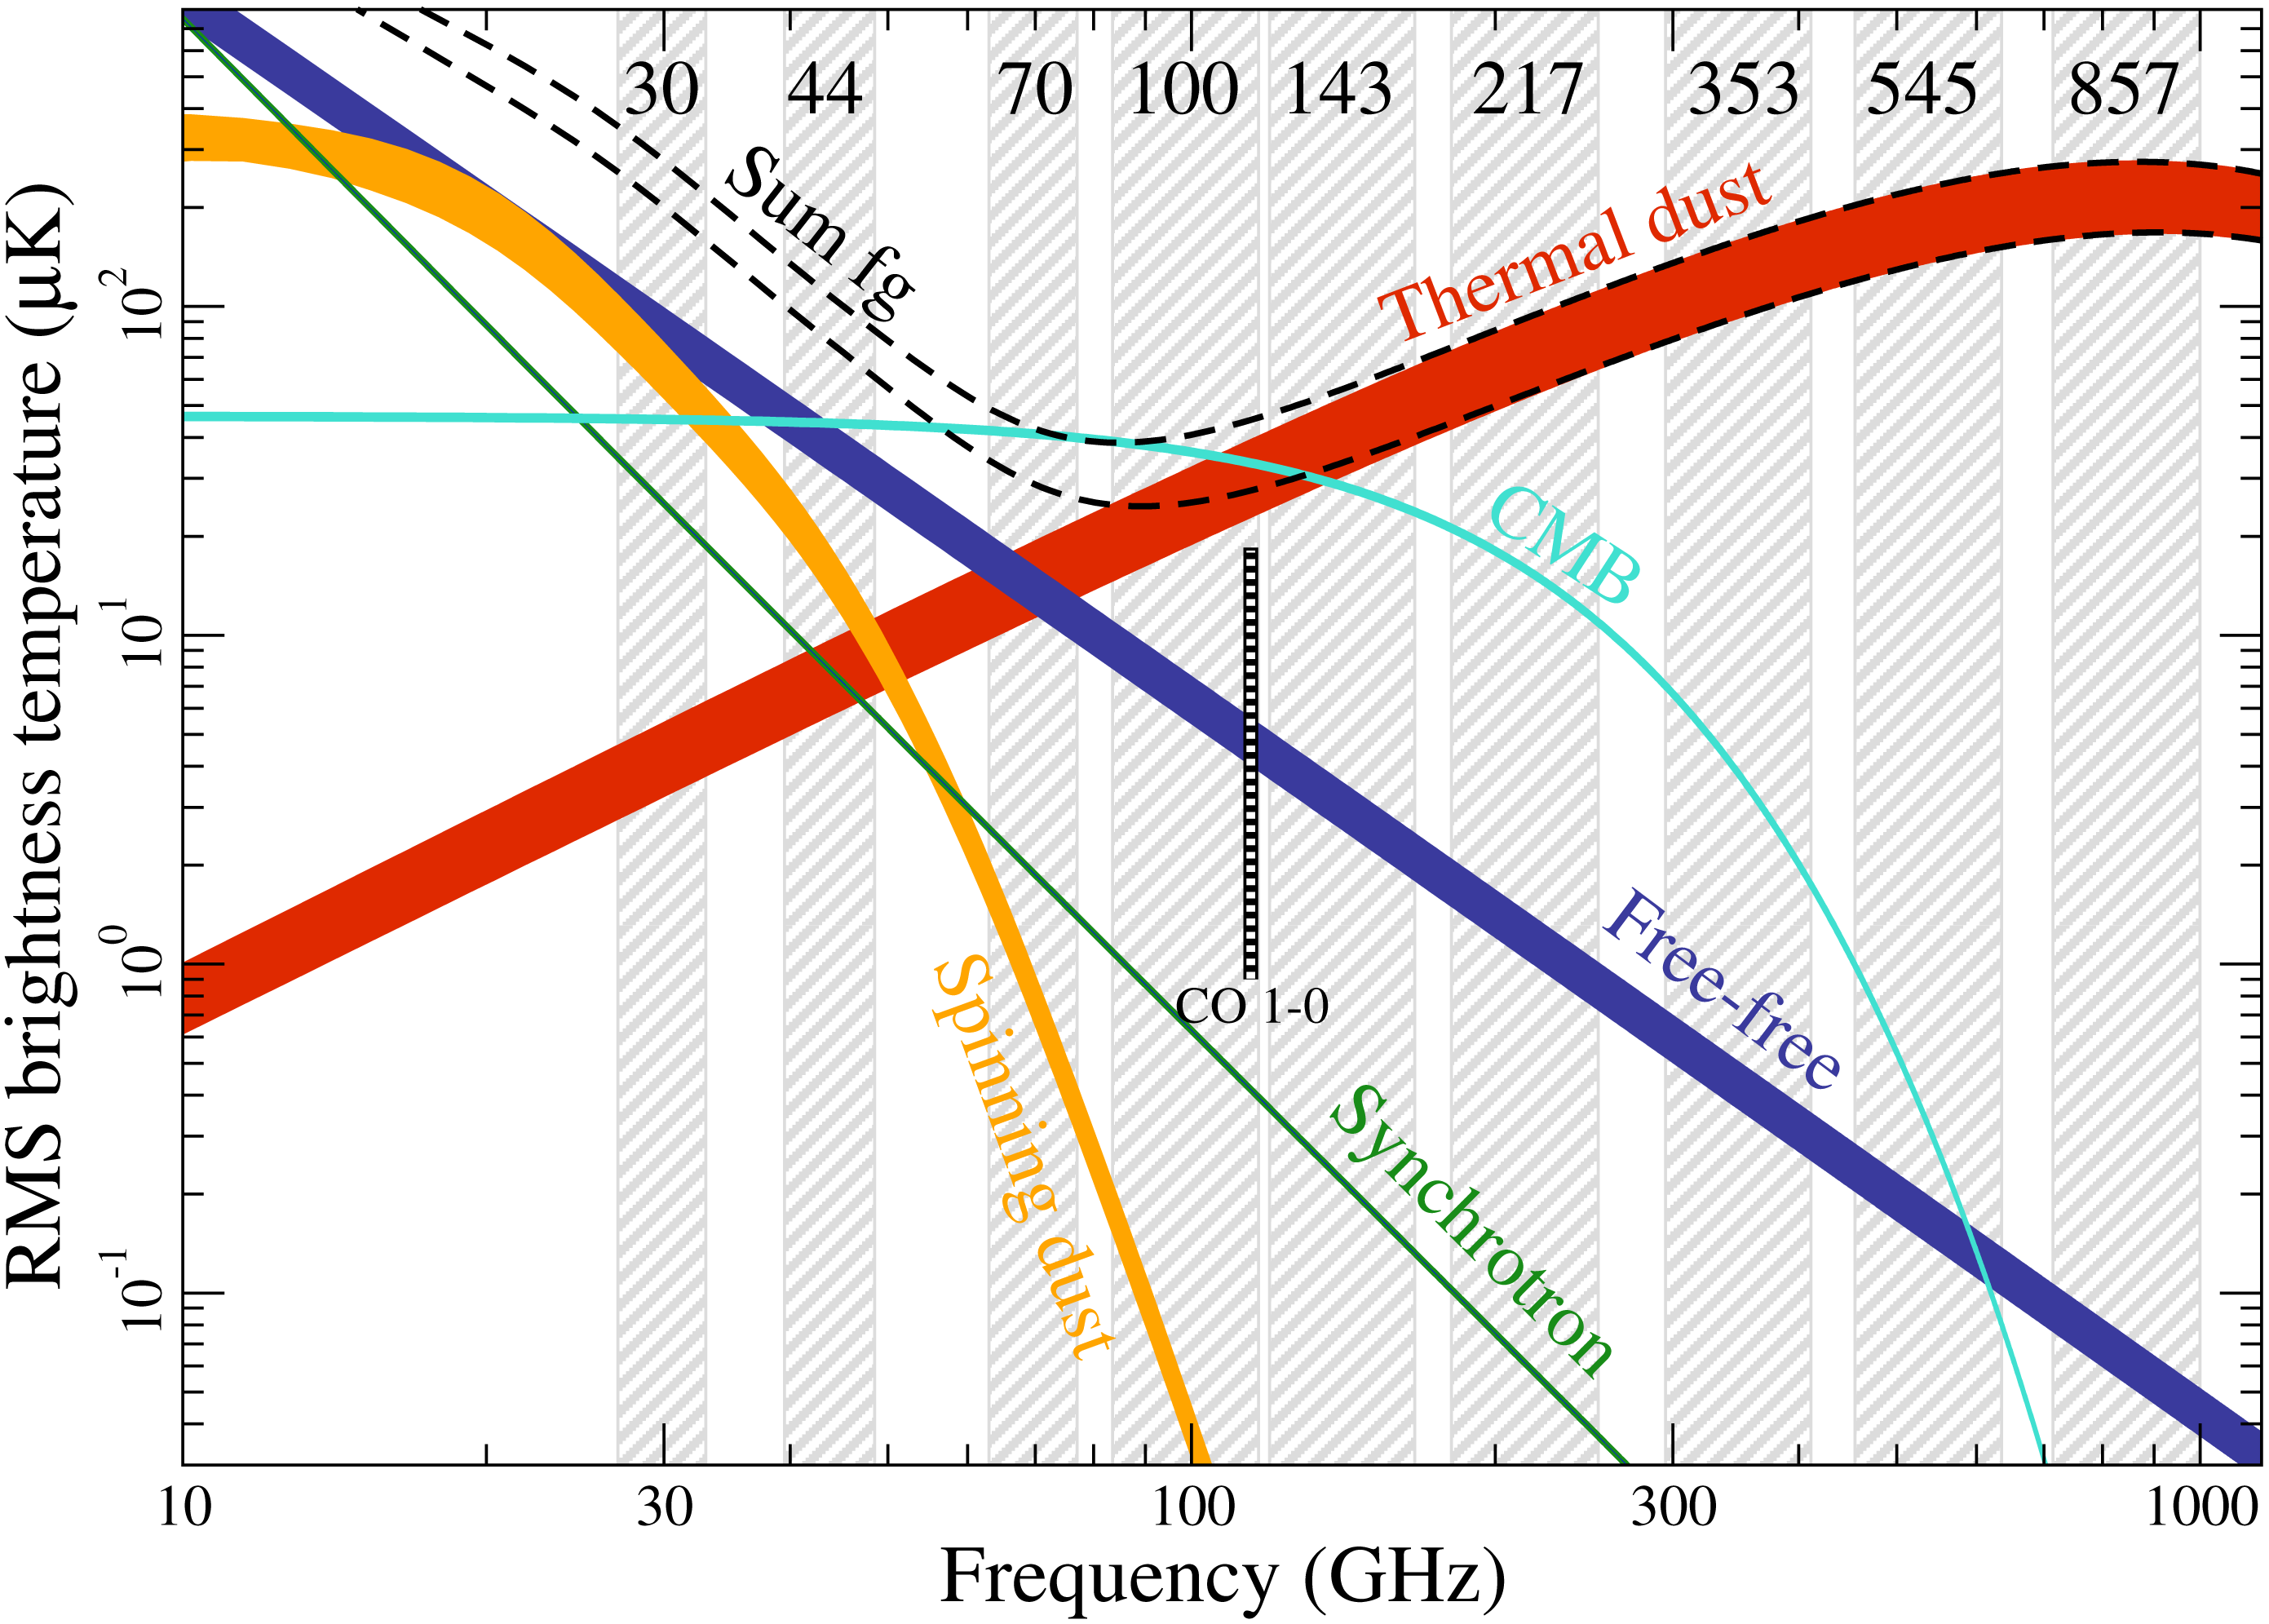
\includegraphics[scale=0.4]{../figures/2015_FGSpectra.png}}
\only<4>{
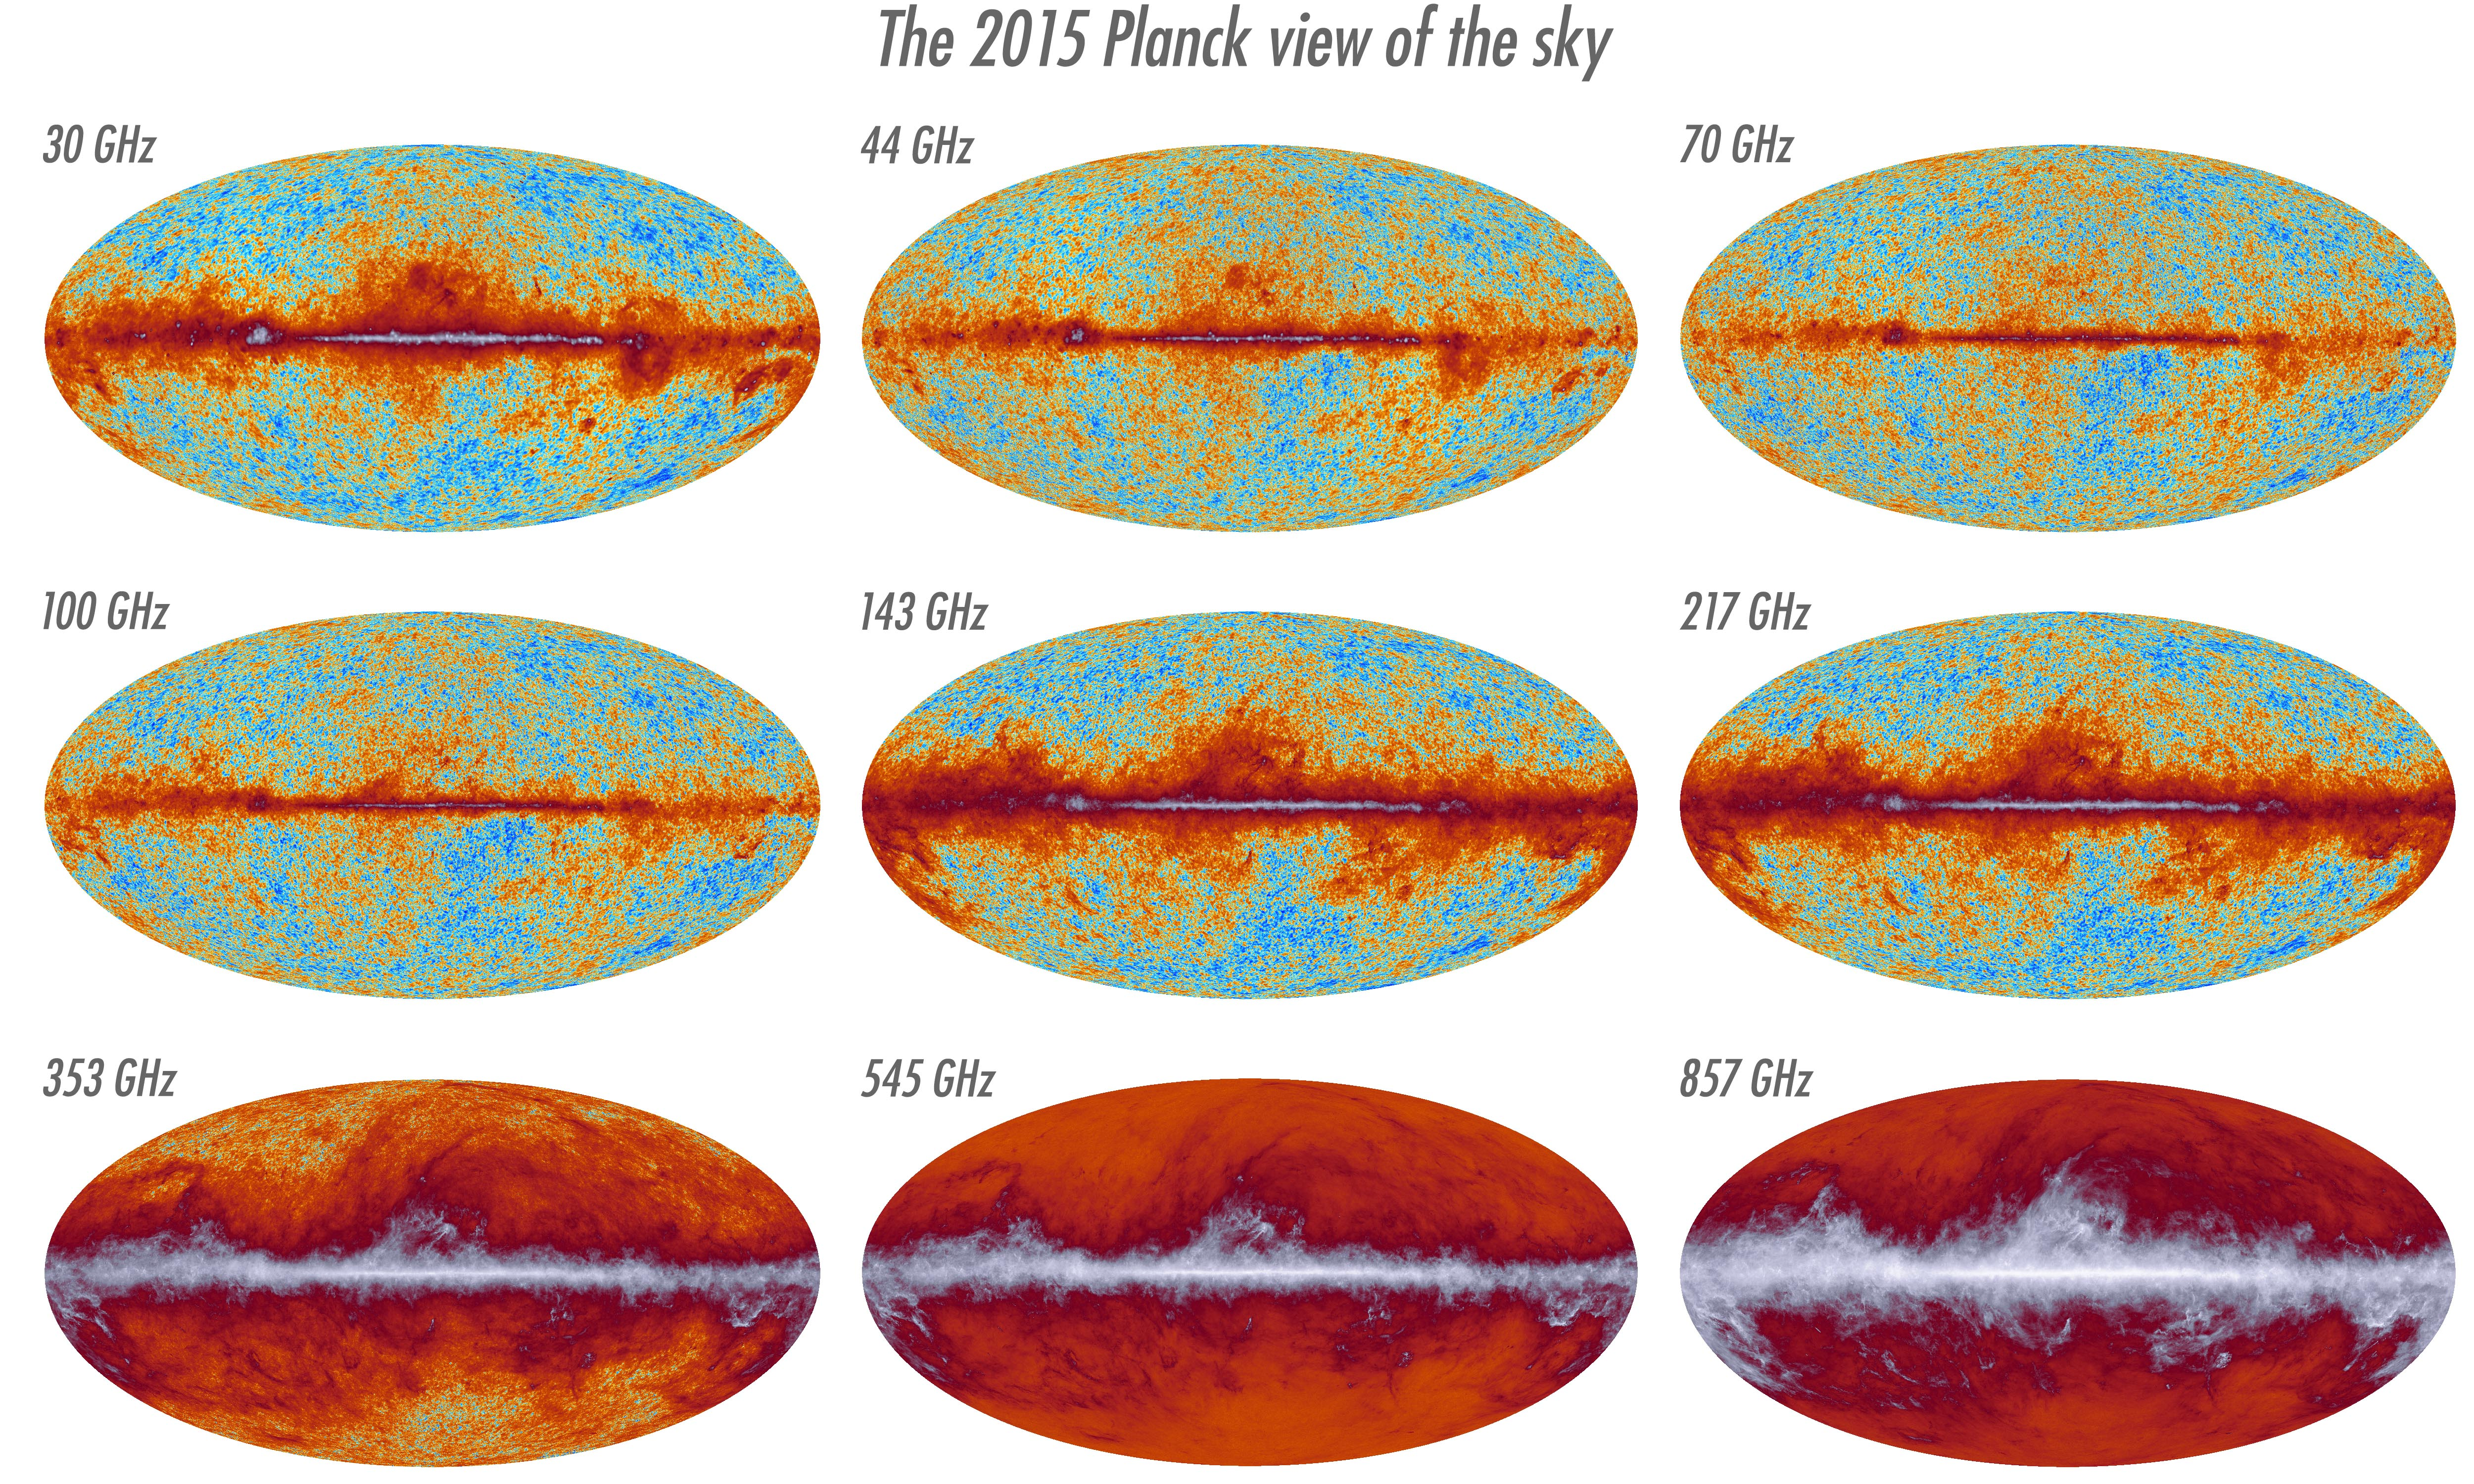
\includegraphics[width=\textwidth]{../figures/9-freqs-2015.jpg}}
\only<6>{
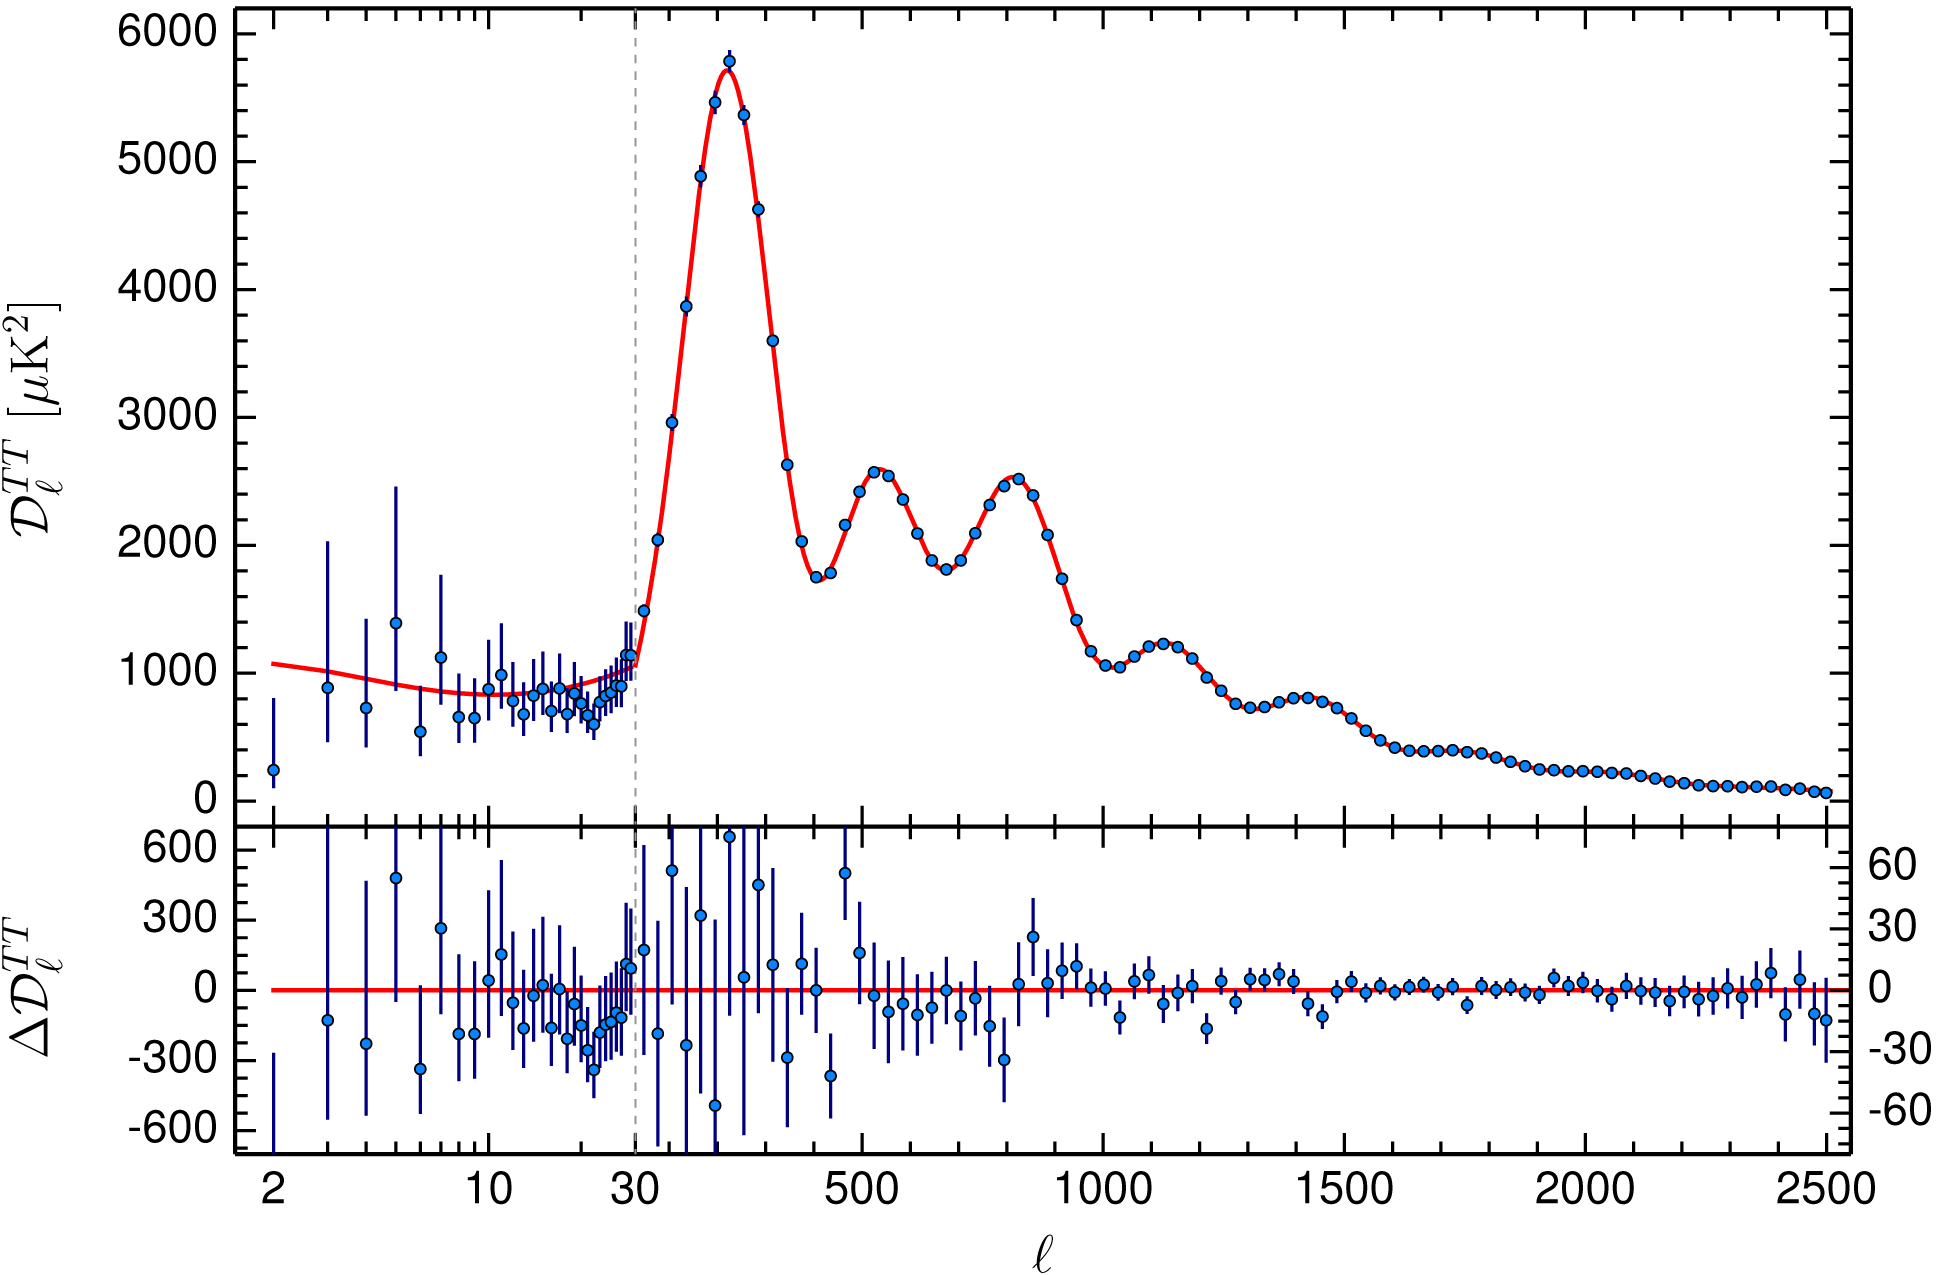
\includegraphics[width=\textwidth]{../figures/2015_TTSpectrum.png}}
\end{figure}
\end{frame}

\begin{frame}{VSK method}
\only<1>{Statistical isotropy is fundamental in the concordance model}
\only<2>{Statistical properties of CMB allow to test assumptions}
\only<3>{CMB anisotropies... isotropic and Gaussian distributed ?} 
\only<4>{Anomalies have been found by WMAP, Planck and other groups}%(e.g., lack of power on large angular scales, alignment of low order multipoles, north-south asymmetry in power spectra, the so-called cold spot)
\only<5>{Unaccounted systematics, non-subtracted foreground contamination, cosmological origin ?}
\only<6>{WMAP and Planck are two independent experiments... unaccounted systematics seems unlikely}
\only<7>{Then, anomalies due to unresolved foreground or cosmological origin ?}
\begin{figure}[hbtp]
\centering
\only<1-7>{
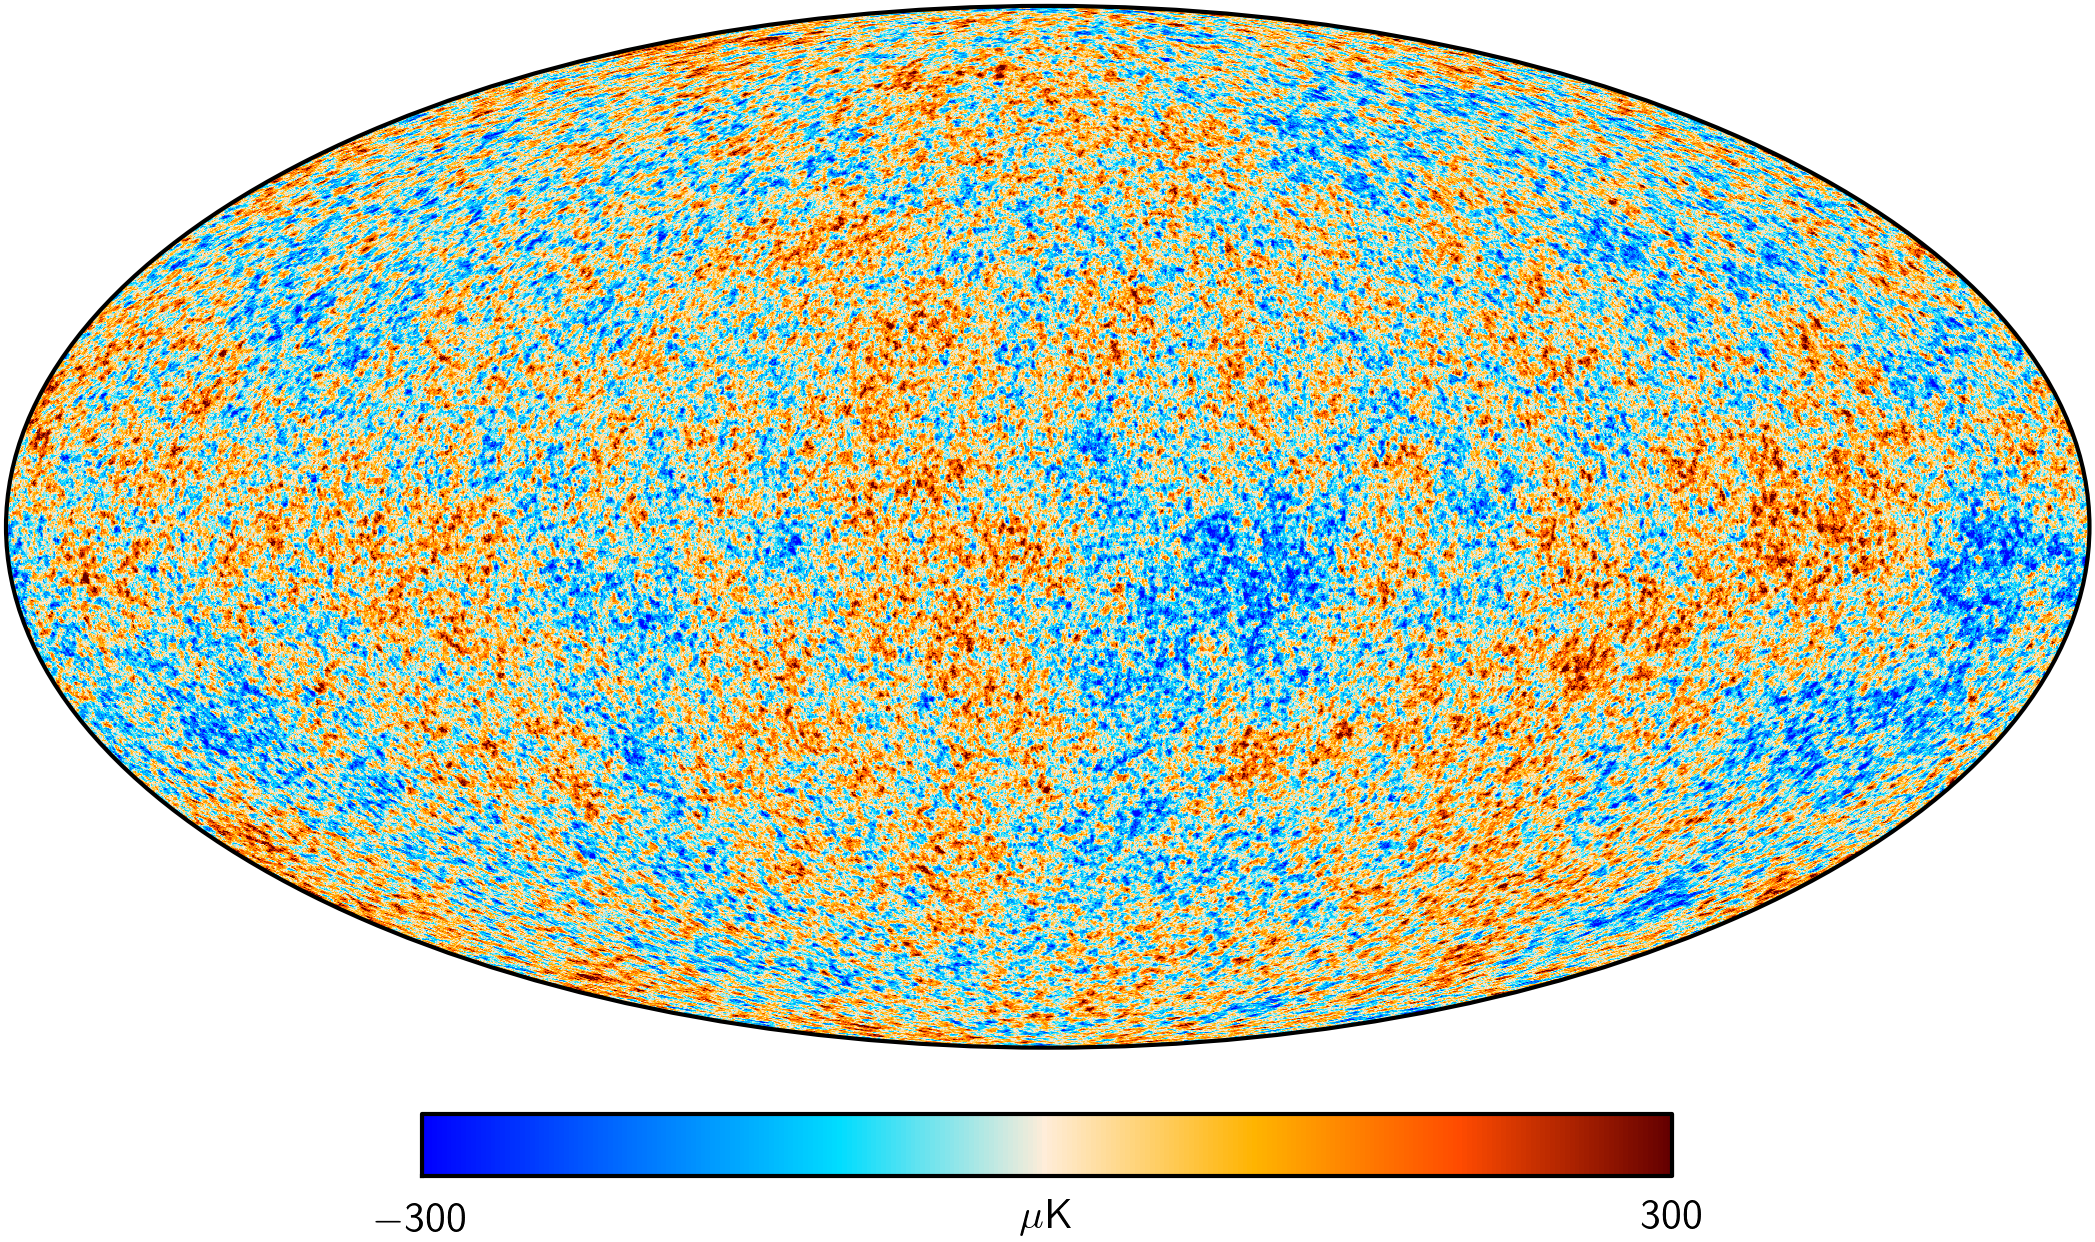
\includegraphics[width=\textwidth]{../figures/2015_SMICA_CMB.png}}
\only<8>{
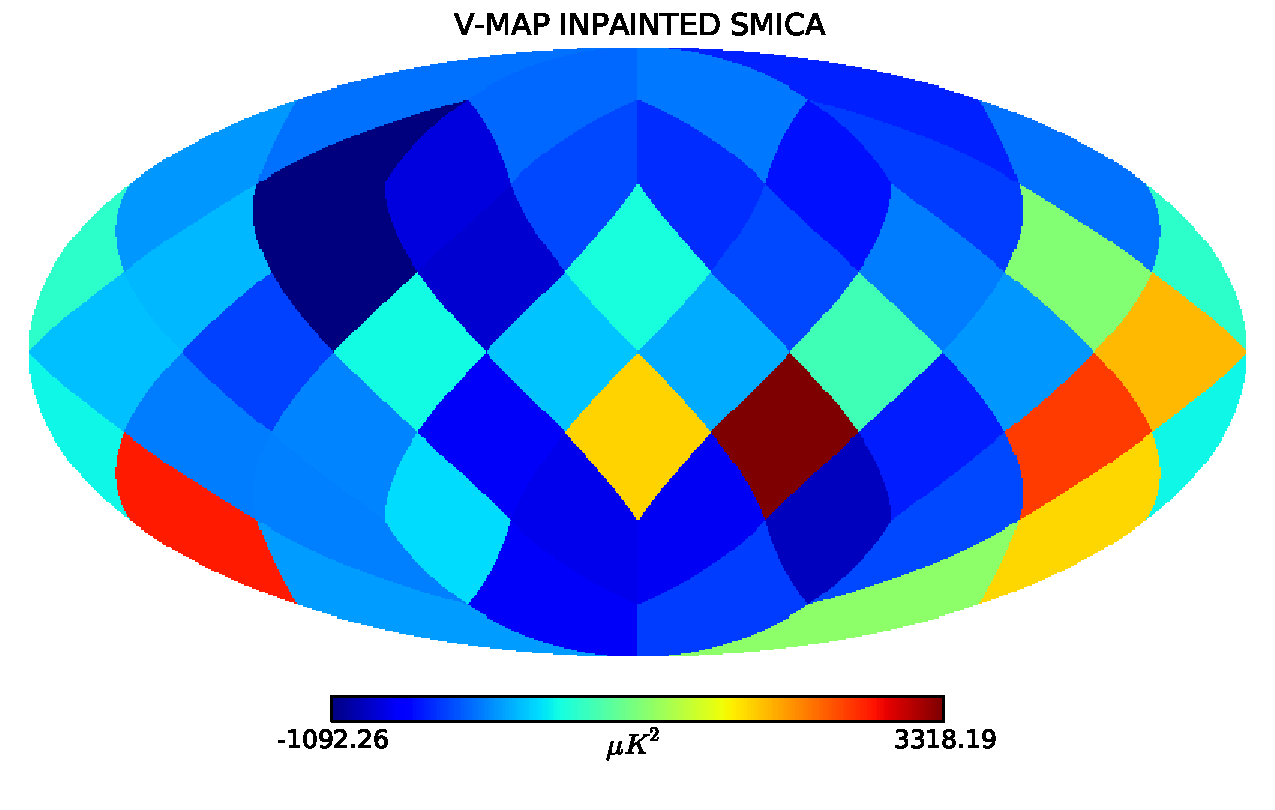
\includegraphics[width=\textwidth]{../figures/chapter-vsk/vmap-inpainted-smica.pdf}}
\only<9>{
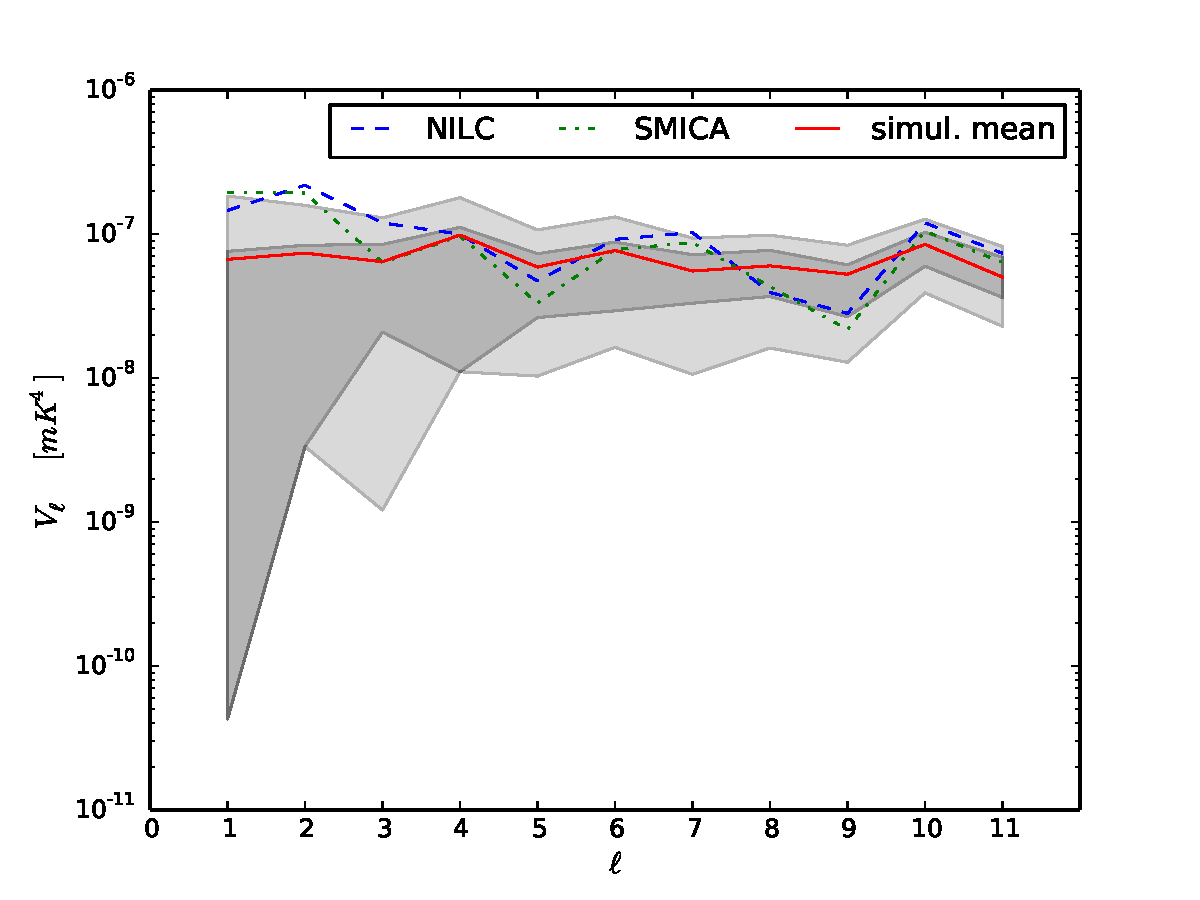
\includegraphics[width=\textwidth]{../figures/chapter-vsk/Inp_Vl.pdf}}
\only<10>{
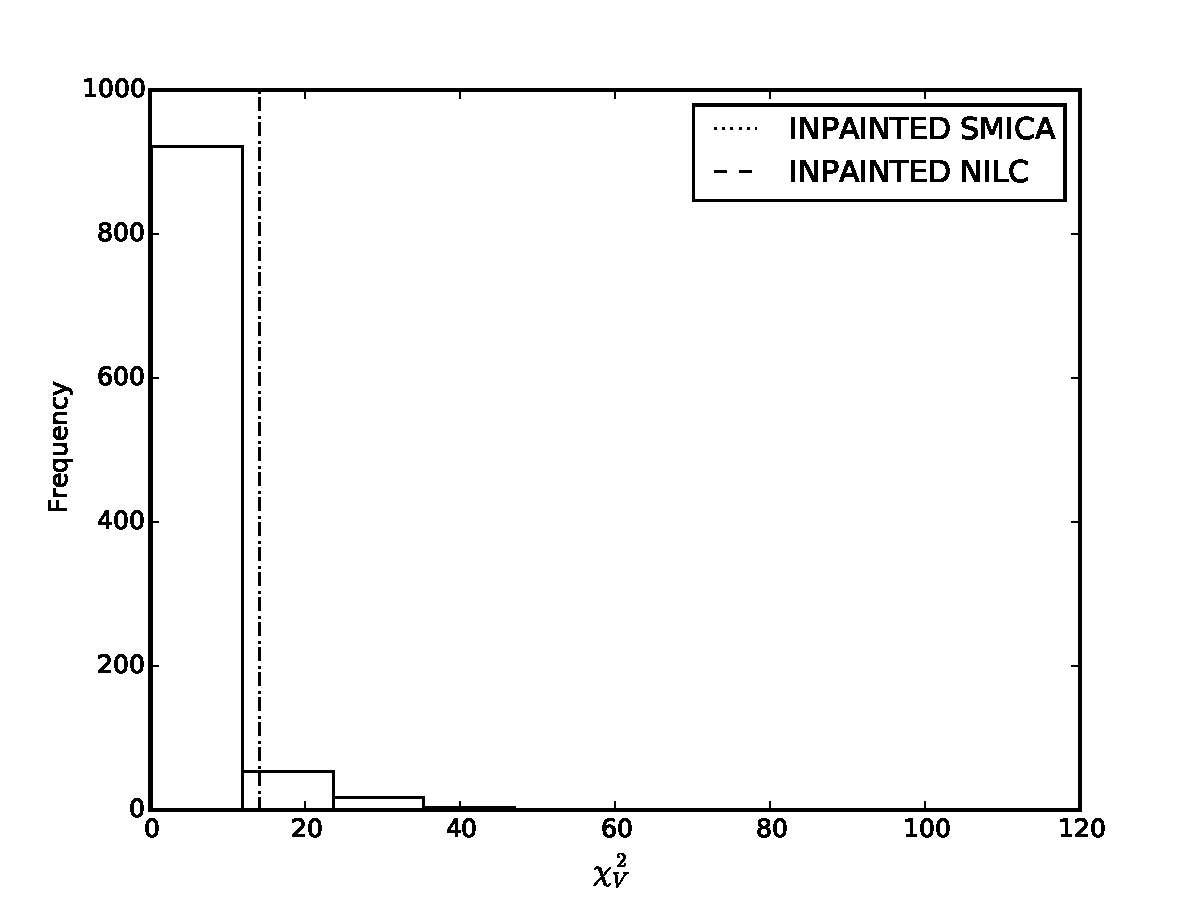
\includegraphics[width=\textwidth]{../figures/chapter-vsk/vchi2.pdf}}
\only<11>{Lower-tail probability for the V, S, K estimators, for the $N_{side} = 2048$ inpainted \texttt{SMICA} and \texttt{NILC}.
\begin{table}
\centering
\begin{tabular}{@{}lcccc}
\hline 
  & & Probability & \\
\hline  
CMB estimate & V & S & K \\ 
\hline  
 & & $N'_{side}=2$ & \\
\texttt{SMICA} & $0.939$ & $0.388$ & $0.096$ \\ 
\texttt{NILC} & $0.939$ & $0.022$ & $1$  \\
 & & $ N'_{side} = 4 $ & \\
\texttt{SMICA} & $ 0.969 $ & $ 0.727 $ & $ 0.521 $ \\
\texttt{NILC} & $ 0.943 $ & $ 0.761 $ & $ 1 $ \\ 
 & & $N'_{side} = 8$ & \\
\texttt{SMICA} & $ 1 $ & $ 0.551 $ & $ 0.581 $ \\
\texttt{NILC} & $ 0.964 $ & $ 0.474 $ & $ 1 $ \\
\hline
\end{tabular} 
\end{table}}
\only<12>{
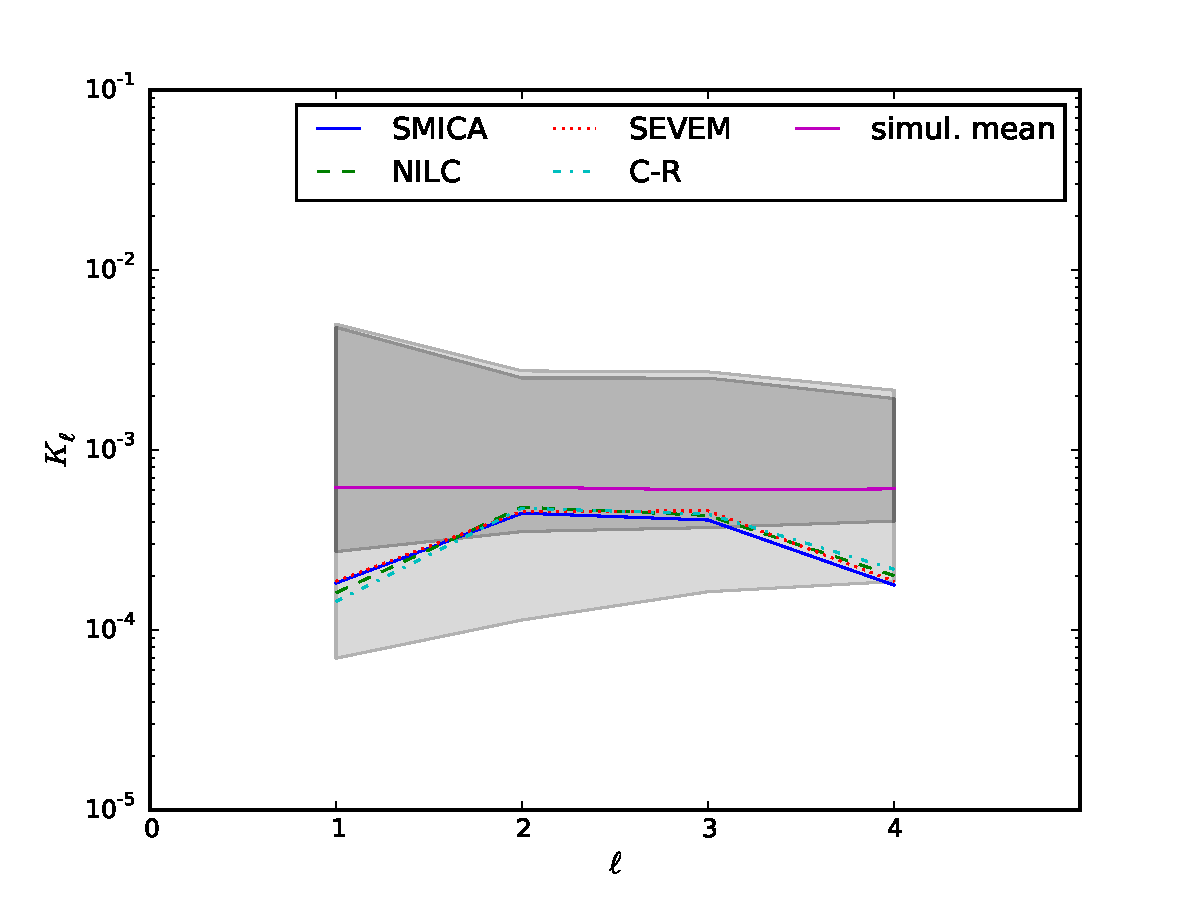
\includegraphics[width=\textwidth]{../figures/chapter-vsk/Kl_u73.pdf}}
\only<13>{\texttt{SMICA} CMB estimate using the U73 mask.
\begin{table}
\centering
\begin{tabular}{@{}lcccc}
\hline 
  & & Probability & \\
\hline  
$N'_{side}$ & V & S & K \\ 
\hline  
 & & $N_{side}=2048$ & \\
$2$ & $0.004 $ & $ 0.024$ & $0.367 $ \\ 
$4$ & $ 0.893 $ & $ 0.407 $ & $ 0.340 $  \\
$8$ & $ 0.695 $ & $ 0.116 $ & $ 0.406 $  \\
 & & $ N_{side} = 1024 $ & \\
$2$ & $ 0.556 $ & $ 0.022 $ & $ 0.281 $ \\ 
$4$ & $ 0.873 $ & $ 0.446 $ & $ 0.229 $  \\
$8$ & $ 0.782 $ & $ 0.117 $ & $ 0.264 $  \\
$16$ & $ 0.442 $ & $ 0.084 $ & $ 0.153 $  \\
\hline
\end{tabular} 
\end{table}
}
\only<14>{\texttt{SMICA} CMB estimate using the U73 mask.
\begin{table}
\centering
\begin{tabular}{@{}lcccc}
\hline 
  & & Probability & \\
\hline  
$N'_{side}$ & V & S & K \\ 
\hline  
 & & $N_{side} = 512$ & \\
$2$ & $0.711 $ & $ 0.027 $ & $ 0.229 $ \\ 
$4$ & $ 0.898 $ & $ 0.485 $ & $ 0.240 $  \\
$8$ & $ 0.794 $ & $ 0.103 $ & $ 0.140 $  \\
$16$ & $ 0.311 $ & $ 0.200 $ & $ 0.146 $  \\
 & & $N_{side} = 256$ & \\
$2$ & $ 0.040 $ & $ 0.123 $ & $ 0.225 $ \\ 
$4$ & $ 0.996 $ & $ 0.480 $ & $ 0.404 $  \\
$8$ & $ 1.0 $ & $ 0.235 $ & $ 0.104 $  \\
$16$ & $ 1.0$ & $ 0.584 $ & $ 0.459 $  \\
\hline
\end{tabular} 
\end{table}
}
\only<15>{\texttt{SMICA} CMB estimate using different masks.
\begin{table}
\centering
\begin{tabular}{@{}lcccc}
\hline 
  & & Probability & \\
\hline  
$N'_{side}$ & V & S & K \\ 
\hline  
 & & U73 ($f_{sky} = 73\%$) & \\
$2$ & $ 0.004 $ & $ 0.024 $ & $ 0.367 $ \\ 
$4$ & $ 0.893 $ & $ 0.407 $ & $ 0.340 $  \\
$8$ & $ 0.695 $ & $ 0.116 $ & $ 0.406 $  \\
 & & VALMASK ($f_{sky} = 89\%$) & \\
$2$ & $ 0.004 $ & $ 0.022 $ & $ 0.357 $ \\ 
$4$ & $ 0.895 $ & $ 0.371 $ & $ 0.343 $  \\
$8$ & $ 0.7 $ & $ 0.099 $ & $ 0.385 $  \\
 & & INP$\_$MASK ($f_{sky} = 97\%$) & \\
$2$ & $ 0.003 $ & $ 0.016 $ & $ 0.382 $ \\ 
$4$ & $ 0.897 $ & $ 0.367$ & $ 0.374 $  \\
$8$ & $ 0.685 $ & $ 0.099 $ & $ 0.428 $  \\
\hline
\end{tabular} 
\end{table}}
\end{figure}
\end{frame}



%\begin{itemize}
%\item 2013 Planck release 
%\item Component separation: Commander-ruler, NILC, SEVEM, SMICA
%\item Inpainted CMB maps: SMICA and NILC
%\item Masks: U73, VALMASK, INPMASK
%\item Different resolution of CMB maps and VSK method
%\item 2000 Gaussian, isotropic CMB maps
%\end{itemize}
%\end{frame}

%\begin{frame}{Project 1: testing a fundamental assumption of the standard model of cosmology}{Why do we care about the cosmological principle ?}
%\begin{itemize}
%\item Statistical isotropy is fundamental in the concordance model
%\item Studying statistical properties of CMB anisotropies we examine assumptions of the standard model
%\item CMB anisotropies... isotropic and Gaussian distributed ? 
%\item Anomalies have been found by WMAP, Planck and other groups (e.g., lack of power on large angular scales, alignment of low order multipoles, north-south asymmetry in power spectra, the so-called cold spot)
%\item Unaccounted systematics, non-subtracted foreground contamination, cosmological origin ?
%\item WMAP and Planck are two independent experiments... unaccounted systematics seems unlikely
%\item Then, anomalies due to unresolved foreground or cosmological origin ?   
%\end{itemize}
%\end{frame}

%\begin{frame}{Project 1: testing statistical isotropy with Planck data}{How do we test Gaussianity and isotropy of the CMB anisotropies ?}
%\begin{itemize}
%\item Utilise the VSK method
%\item Works in real space: localising possible non-subtracted foregrounds, may provide angular scale of possible deviations of Gaussianity and isotropy
%\item Remove both monopole and dipole from CMB maps
%\item Superimpose on the CMB map a Healpix grid with much lower resolution
%\item For each new pixel, compute sample variance, sample skewness, and sample kurtosis 
%\item The result is three functions on the sphere: a map of sample variance, a map of sample skewness, and a map of sample kurtosis
%\item Repeat the above procedure for data and Gaussian isotropic simulations
%\item Compute zero mean maps (variance, skewness, and kurtosis)
%\item Compute angular power spectrum of the resulting maps
%\item Quantify the degree of agreement data and Gaussian simulations through a $\chi^2$ test for each kind of map 
%\end{itemize}
%\end{frame}



%\begin{frame}{Project 1: testing statistical isotropy with Planck data}{Results}
%\begin{itemize}
%\item Example of V-map
%\item Example of angular power spectrum
%\item Example of $\chi^2$ test
%\item Table summarising results for inpainted maps
%\item Table summarising dependence on CMB map resolution and VSK method resolution
%\item Table dependence on the sky fraction
%\item Figure comparison component separation
%\end{itemize}
%\end{frame}

%\begin{frame}{Project 1: testing a fundamental assumption of the standard model of cosmology}

%\end{frame}

\setbeamercolor{frametitle}{bg=aquamarine}

\section*{Project 2: constraints on anisotropic dark energy}

\begin{frame}{Why do we care about anisotropic dark energy ?}
\begin{itemize}
\item No clear explanation for the accelerating expansion of the universe
\item Two leading approaches: an unobserved fluid dubbed dark energy (DE) or modify Einstein's theory of gravity on large scales
\item A general fluid can be characterised by equation of state, sound speed, and anisotropic stress
\item Literature has focused on the background evolution, but what about DE perturbations ?  
\item Anisotropic stress is a key feature: it allows to distinguish standard DE model ($\Pi_{\rm de} = 0$) from modified gravity models ($\Pi_{\rm de}\neq 0$)
\end{itemize}
\end{frame}

\begin{frame}{How do we constrain anisotropic stress ?}
\begin{itemize}
\item Adopt a phenomenological approach: a DE model including a range of approaches
\item Find approximate solutions for DE perturbations
\item Implement the model in CAMB and do MCMC with COSMOMC 
\item Data from Planck, BAO, supernovae, but exclude $P(k)$ and $H_0$
\end{itemize}
\end{frame}

\begin{frame}{Results}
\begin{itemize}
\item The effect of anisotropic stress on CMB angular power spectrum and on the matter power spectrum
\item Constrains do not show evidence of non-zero anisotropic stress. 
\end{itemize}
\end{frame}

\begin{frame}{Project 2: constraints on anisotropic dark energy}
\begin{figure}[hbtp]
\centering
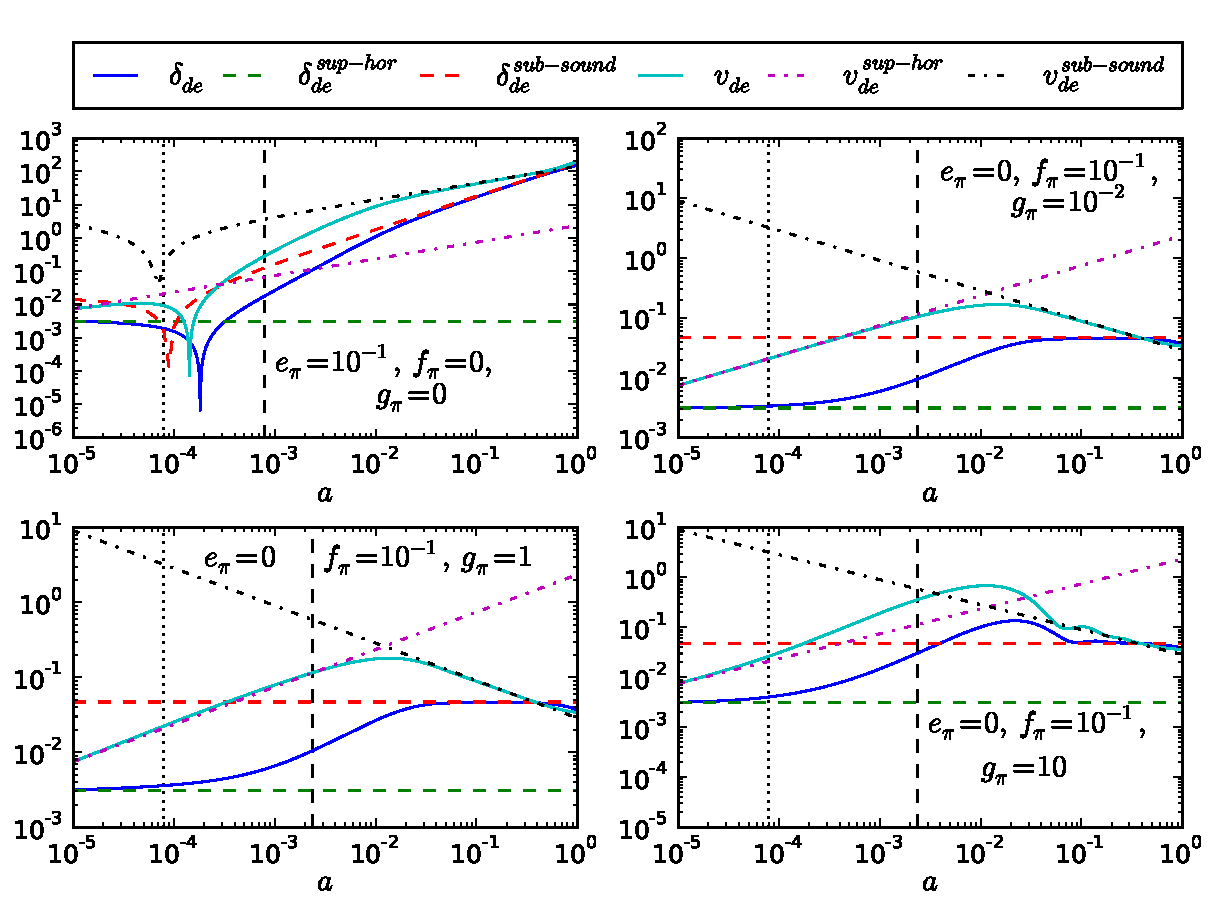
\includegraphics[width=\textwidth]{../figures/chapter-ade/comparison.pdf}
\end{figure}

\end{frame}

\begin{frame}{Project 2: constraints on anisotropic dark energy}
\begin{figure}[hbtp]
\centering
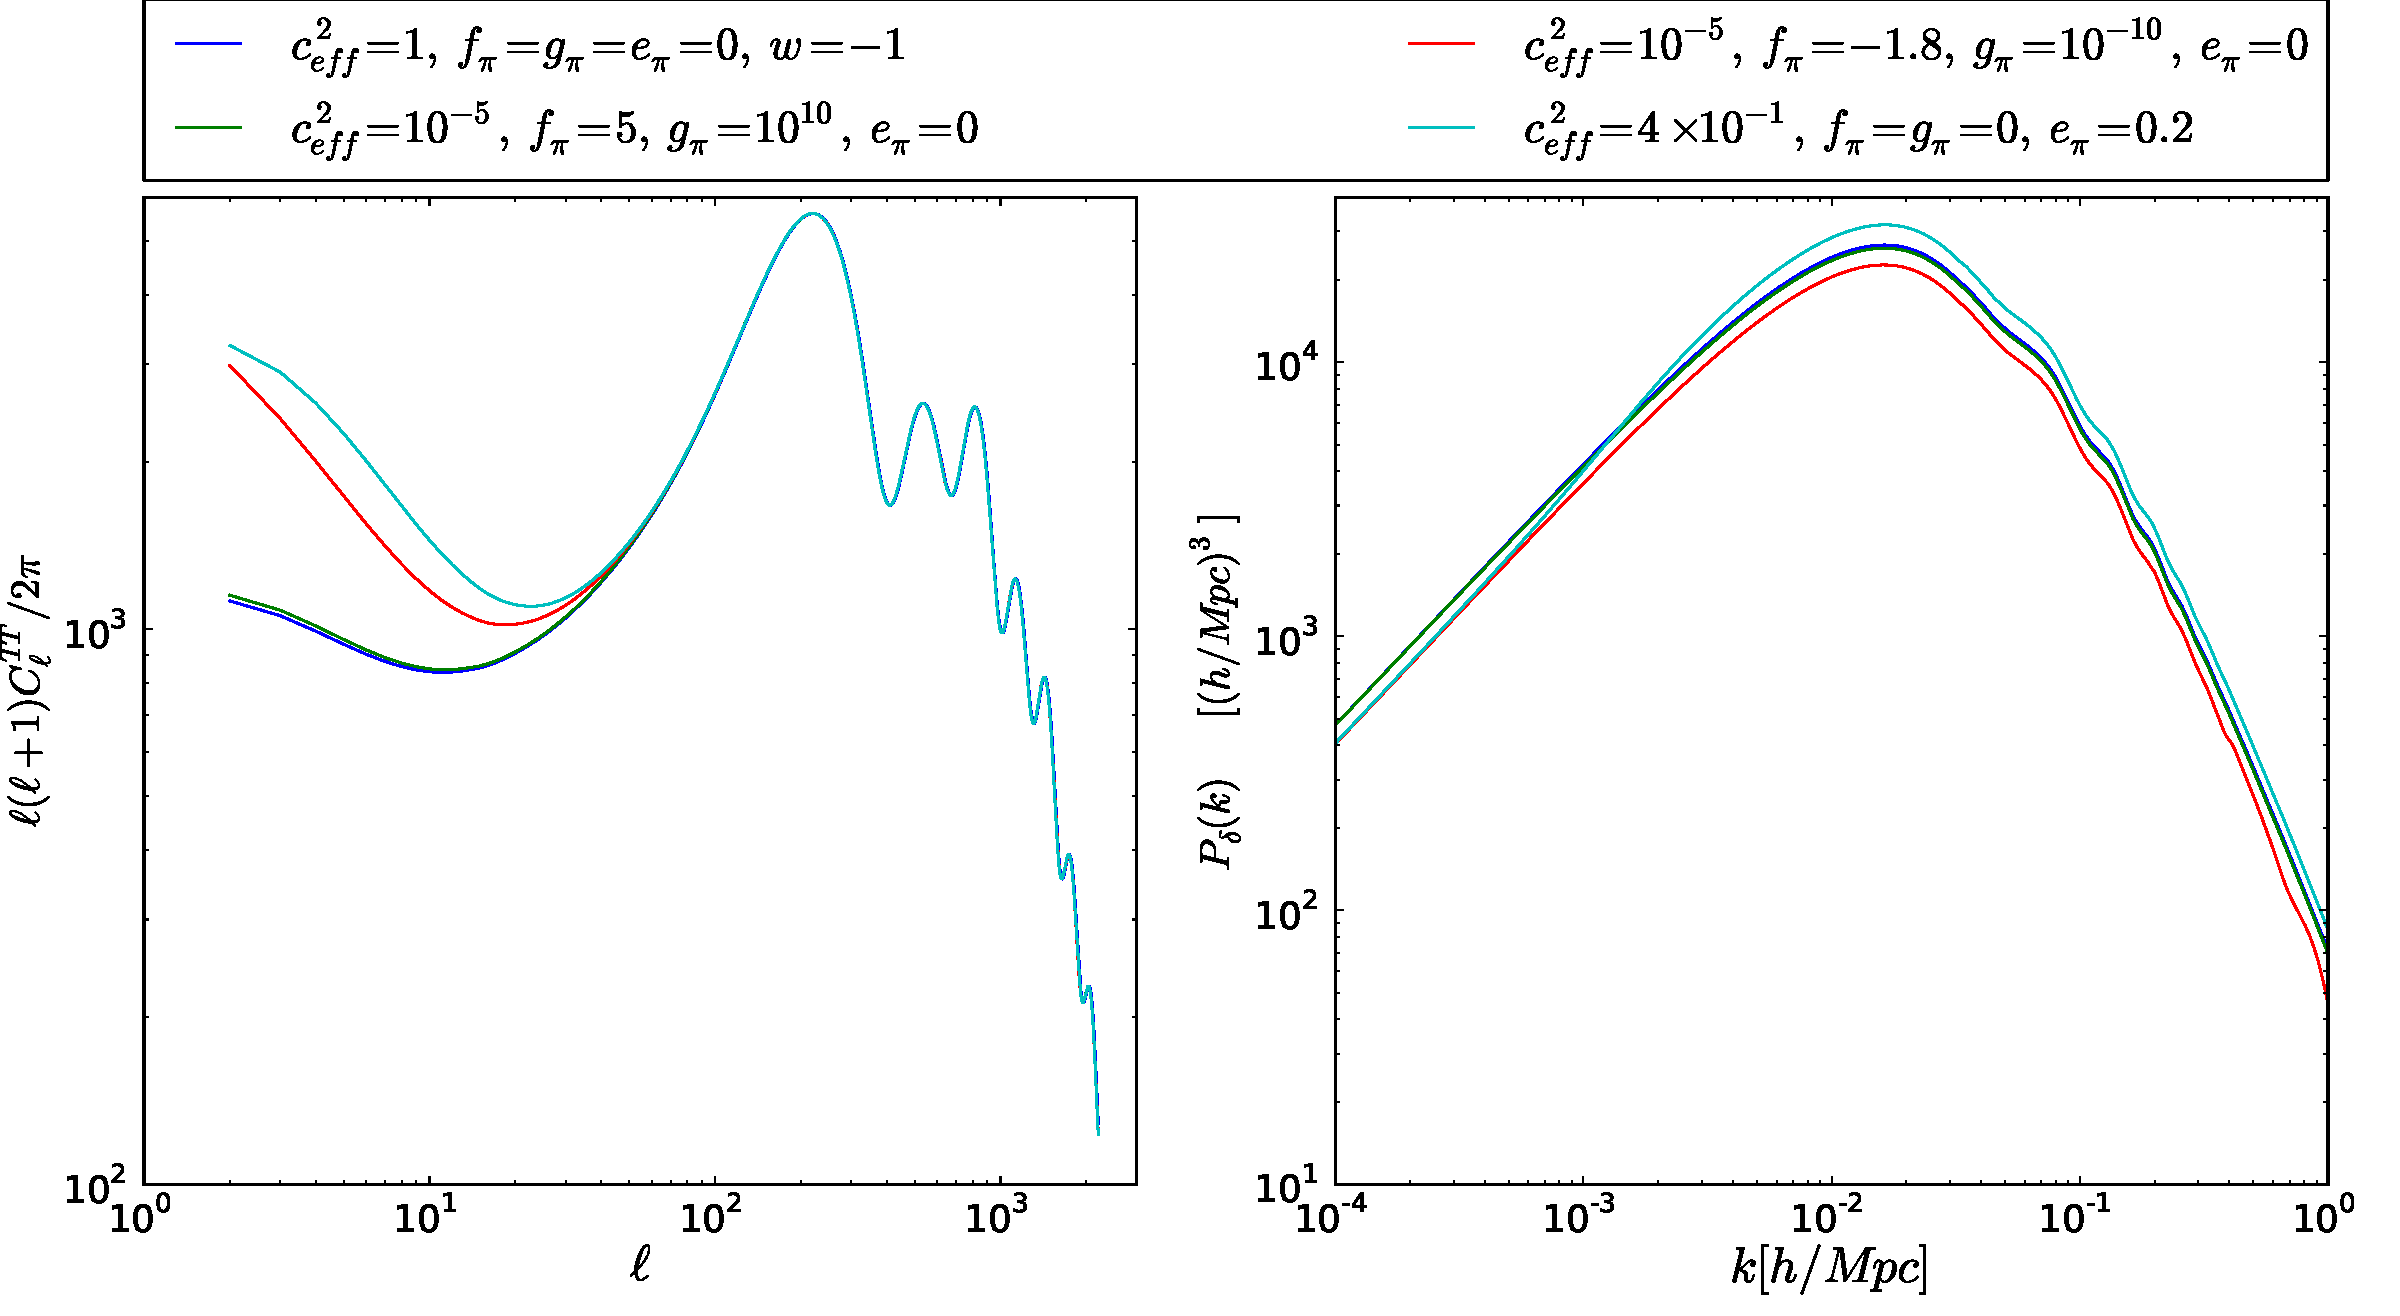
\includegraphics[width=\textwidth]{../figures/chapter-ade/PkCls_2.pdf}
\end{figure}
\end{frame}

\begin{frame}{Project 2: constraints on anisotropic dark energy}
\begin{figure}[hbtp]
\centering
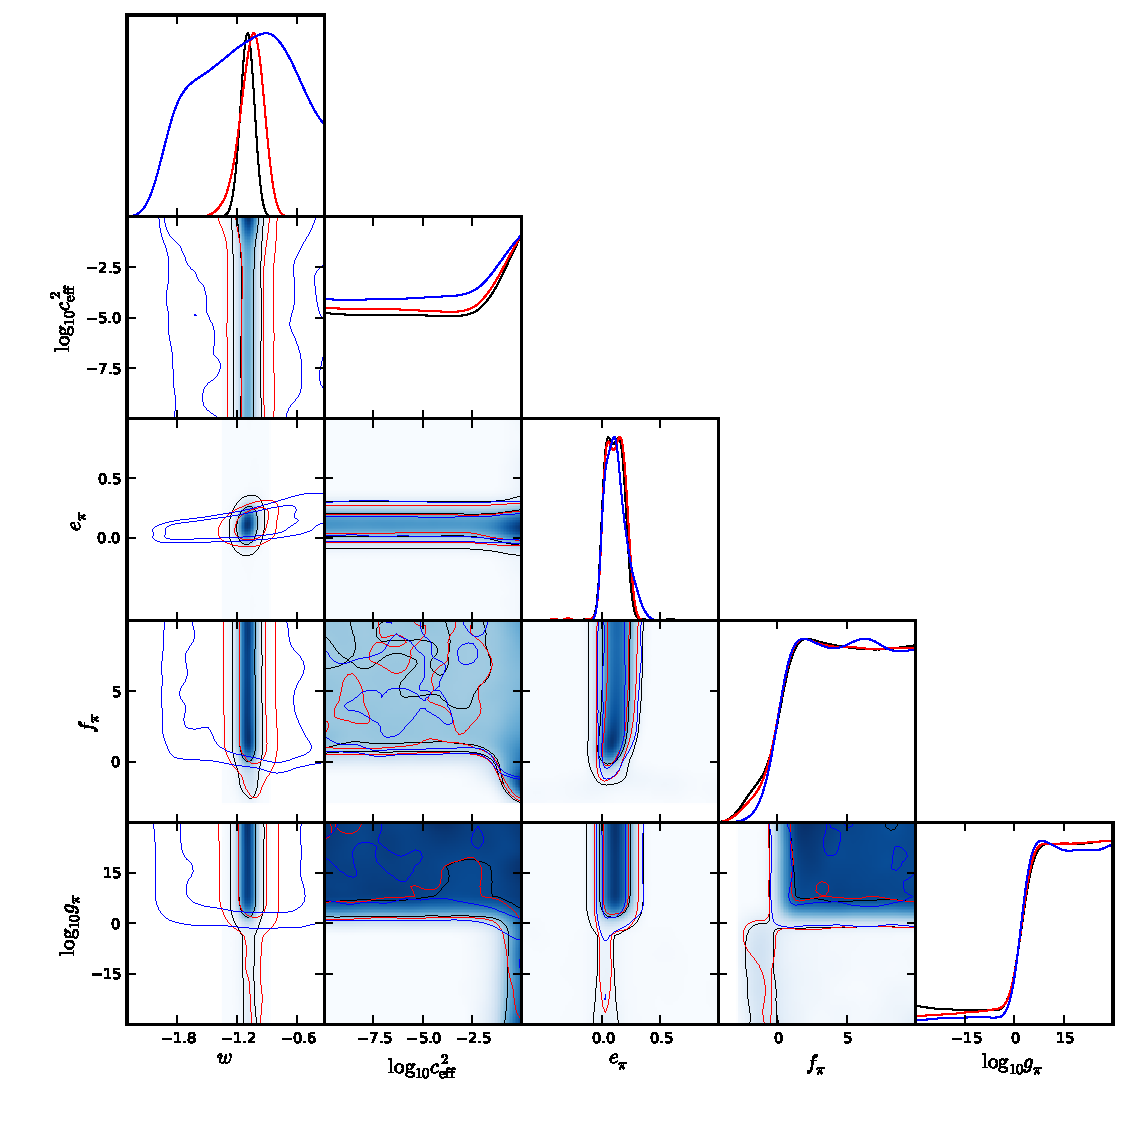
\includegraphics[width=0.8\textwidth]{../figures/chapter-ade/PWHiBSwefc_tri.pdf}
\end{figure}

\end{frame}

\setbeamercolor{frametitle}{bg=orange}

\section*{Project 3: upcoming galaxy surveys, the lensing convergence and the neutrino mass}

\begin{frame}{Why do we care about massive neutrinos ?}
\begin{itemize}
\item Underlying physics in the standard model of cosmology remains unknown
\item Cold Dark Matter (CDM) constitutes  about $30\%$ of the energy content
\item Neutrinos are the only known dark matter candidate
\item Neutrinos are massive, but their absolute scale remains unconstrained
\end{itemize}
\end{frame}

\begin{frame}{How do we observe the effect of massive neutrinos ?}
\begin{itemize}
\item Signatures of massive neutrinos in observations: CMB anisotropies and galaxy distribution
\item Neutrinos change background evolution. For small neutrino masses, CMB can only provide upper limit 
\item Degeneracies degrade constraints from CMB data
\item Galaxy surveys come in to the rescue: probe low red-shift universe, break degeneracies
\item Massive neutrinos suppress clustering of galaxies at small scales, future surveys will hopefully take advantage of this
\item Upcoming surveys will probe distances comparable to the Hubble horizon: relativistic effects must be consistently included in the analysis
\end{itemize}

\end{frame}

\begin{frame}{Galaxy number counts angular power spectrum $C_\ell(z,z')$}
\begin{itemize}
\item $P(k,z)$ is not an observable. $C_\ell(z,z')$ is an observable
\item Galaxy number counts for a survey with limiting magnitude
\item Expand in spherical harmonics, taking into account red-shift dependence
\item Assume statistical isotropy and compute angular power spectrum 
\item In practice, divide the catalogue in red-shift bins 
\end{itemize}
\end{frame}

\begin{frame}{How do we estimate the importance of neglecting lensing convergence ?}
\begin{itemize}
\item Fit a model neglecting the effect to data 
\item Fit a model neglecting the effect to data, but only use auto-correlations (close to $P(k)$ analysis)
\item Fit a model consistently including the effect 
\item Conservative treatment of non-linearities
\item Include shot-noise (galaxy distribution is not a continuous field)
\item Number counts alone 
\item Number counts and use CMB information from Planck
\end{itemize}
\end{frame}

\begin{frame}{Results}
\begin{figure}[hbtp]
\centering
\includegraphics[width=0.75\textwidth]{../figures/chapter-mnu/triangle_figure_MCDM_bias_cmb_prior.pdf}
\end{figure}

\end{frame}

\begin{frame}{Results}
\begin{figure}[hbtp]
\centering
\includegraphics[width=0.9\textwidth]{../figures/chapter-mnu/fid_shift.pdf}
\end{figure}

\end{frame}

%\begin{frame}{Results}
%\begin{itemize}
%\item Table showing biased parameters: spurious detection of neutrino mass
%\item Plot showing auto- and cross-correlations, equation showing dominant contribution
%\item Lensing convergence must be included in the analysis of upcoming galaxy surveys, with appropriate magnification bias
%\end{itemize}
%\end{frame}

%\begin{frame}{Two important observational facts from the past century}
%\only<1>{The Universe is expanding (1929)}
%\only<2>{The Universe is expanding (1929): $v \propto D = a(t) d$ }
%\only<3>{The Universe is speeding up (1998): $\ddot{a(t)}>0$}
%\begin{figure}[hbtp]
%\centering
%\only<1>{
%\includegraphics[width=\textwidth]{../figures/doppler_effect.jpg}} 
%\only<2>{
%\includegraphics[width=\textwidth]{../figures/Hubble-law.pdf}}
%\only<3>{
%\includegraphics[scale=0.4]{../figures/Union21_Hubble_slide.pdf}}
%\end{figure}
%\end{frame}

%\begin{frame}{Gravity}
%\only<1>{General Relativity: (geometry) $G_{\mu\nu} \propto T_{\mu\nu} $ (energy)}
%\only<2>{Matter collapses}
%\begin{figure}[hbtp]
%\centering
%\only<1>{
%\includegraphics[width=0.6\textwidth]{../figures/GR.jpg} 
%}
%\only<2>{
%\includegraphics[width=0.9\textwidth]{../figures/galaxyevolution.jpg} 
%} 
%\end{figure}
%\end{frame}

%\begin{frame}{Flatness and isotropy}
%\only<1>{Possible geometries in the standard model}
%\only<2>{Planck constrains $|\Omega_K|<0.005$}
%\only<3>{CMB is very isotropic: $\Delta T << \bar{T}=2.7$K}
%\begin{figure}[hbtp]
%\centering
%\only<1>{
%\includegraphics[width=0.6\textwidth]{../figures/flatness.jpg}}
%\only<2>{
%\includegraphics[width=\textwidth]{../figures/2015_TTSpectrum.png}}
%\only<3>{
%\includegraphics[width=\textwidth]{../figures/2015_SMICA_CMB.png}
%}
%\end{figure}
%\end{frame}

%\begin{frame}{Visible matter}
%\only<2>{$\sum m_\nu$ ?}
%\begin{figure}[hbtp]
%\centering
%\only<1>{
%\includegraphics[width=\textwidth]{../figures/Timeline_portrait.jpg}}
%\only<2>{
%\includegraphics[width=0.6\textwidth]{../figures/standard_model_ai_s2.png} 
%}
%\end{figure}
%\end{frame}

%\begin{frame}{Dark Matter and Dark Energy}
%\only<2>{$\nu$ are the only known DM candidates}
%\only<3>{Since DE dominates now, its pressure must be negative}
%\begin{figure}[hbtp]
%\centering
%\only<1>{
%\includegraphics[width=\textwidth]{../figures/2015_TTSpectrum.png}}
%\only<2>{
%\includegraphics[width=0.8\textwidth]{../figures/Planck-only_Cosmic-recipe-pie-chart.jpg} 
%}
%\only<3>{
%\includegraphics[width=0.4\textwidth]{../figures/dark-energy-4.jpg} 
%}
%\end{figure}
%\end{frame}

%\begin{frame}{A few shortcomings}
%\begin{itemize}
%\item Flatness ($|\Omega_K|<0.005 $) ? 
%\item Horizon 
%\item What is the origin of the density perturbations $\delta \rho_i/\rho_i$ we observe today: (e.g., CMB anisotropies, galaxies) ? 
%\end{itemize}
%\end{frame}

%\begin{frame}{Inflation}
%\only<1>{The potential energy of an evolving scalar field would have dominated the energy content in the very early universe, so that its pressure was negative and $\ddot{a(t)}>0$}
%\only<2>{Quantum fluctuations of the scalar field would have seeded the density perturbations we see today: CMB anisotropies and LSS}  
%\begin{figure}[hbtp]
%\centering
%\only<1>{
%\includegraphics[width=0.9\textwidth]{../figures/fig_horizon_problem_inflation_simp.png}}
%\only<2>{
%\includegraphics[width=0.7\textwidth]{../figures/quantum-fluctuations.jpg}
%}
%\end{figure}
% 
%\end{frame}

%\begin{frame}{$\Lambda$CDM phenomenologically successful, but...}
%\only<1>{What is DM ? and $\sum m_\nu$ ?}
%\only<2>{What is driving the accelerating expansion of the Universe ? DE ? Modified gravity ?} 
%\only<3>{What mechanism produced inflation ?} 
%\only<4>{To what extent are valid the assumptions of the standard model ?}
%\begin{figure}[hbtp]
%\centering
%\only<1-4>{
%\includegraphics[width=0.7\textwidth]{../figures/Timeline_portrait.jpg}}
%\end{figure}
%\end{frame}

%\begin{frame}
%\begin{figure}[hbtp]
%\centering
%\setlength{\unitlength}{0.1\textwidth}
%\begin{picture}(10,7)
%\only<1-21>{
%\put(0,0){\includegraphics[width=\textwidth]{../figures/Timeline_portrait.jpg}}}
%\only<1>{
%\put(0.5,6.5){\wct{Recent observations}}}
%\only<2>{
%\put(0.5,6.5){\wct{Expanding universe}}}
%\only<3>{
%\put(0.5,6.5){\wct{Accelerating expansion}}}
%\only<4>{\put(0.5,6.5){\wct{Flatness, isotropic, tiny $\Delta T/T$}}}
%\only<5>{\put(0.5,6.5){\wct{No evidence of charge asymmetry}}}
%\only<6>{\put(0.5,6.5){\wct{GR: geometry $\propto$ energy}}}
%\only<7>{\put(0.5,6.5){\wct{Gravity: Matter clusters}}}
%\only<8>{\put(0.5,6.5){\wct{Visible matter and the SM ($4.9\%$)}}}
%\only<9>{\put(0.5,6.5){\wct{Neutrinos}}}
%\only<10>{\put(0.5,6.5){\wct{$\sum m_\nu$ ?}}}
%\only<11>{\put(0.5,6.5){\wct{Dark matter (DM, $26.8\%$) and Dark Energy (DE, $68.3\%$)}}}
%\only<12>{\put(0.5,6.5){\wct{DM evidence ?}}}
%\only<13>{\put(0.5,6.5){\wct{$\sum m_\nu$ and DM}}}
%\only<14>{\put(0.5,6.5){\wct{DE $p<0$ and late-time acceleration}}}
%\only<15>{\put(0.5,6.5){\wct{Origin of $\delta \rho_i/\rho_i$, flatness, horizon ?}}}
%\only<16>{\put(0.5,6.5){\wct{Inflation: horizon}}}
%\only<17>{\put(0.5,6.5){\wct{Inflation: flatness}}}
%\only<18>{\put(0.5,6.5){\wct{Inflation: quantum fluctuations}}}
%\only<19>{\put(0.5,6.5){\wct{More questions: DM ? $\ddot{a}>0$ ? Inflation ? $\Lambda$CDM assumptions ?}}}
%\only<20>{\put(0.5,6.5){\wct{Upcoming galaxy surveys}}}
%\only<21>{\put(0.5,6.5){\wct{Statistical properties of data and model predictions}}}
%\end{picture}
%\end{figure}
%
%\end{frame}


%\section{Brief introduction: the concordance model of cosmology}

%\begin{frame}{Brief introduction: the concordance model of cosmology}{The expanding universe}
%\begin{itemize}
%\item Cosmological principle
%\item No charge asymmetry
%\item General relativity
%\item Solutions for Einstein's field equations satisfying the cosmological principle
%\item The universe is expanding...
%\item also speeding up!
%\item Matter described by standard model of particle physics is not enough to match observations
%\end{itemize}
%\end{frame}

%\begin{frame}{Brief introduction: the concordance model of cosmology}{inflation + $\Lambda$CDM}
%\begin{itemize}
%\item Need Dark Matter and Dark Energy to fit the accelerating expansion
%\item Universe looks flat and is not completely homogeneous
%\item Inflationary epoch sets adequate initial conditions for the standard model
%\item So, what is DM and what is driving the accelerating expansion ? and what mechanism produced an inflationary period in the early universe ?
%\item Several possible answers 
%\end{itemize}
%\end{frame}

%\begin{frame}{Brief introduction: the concordance model of cosmology}{Vanilla model of cosmology lacks in fundamental grounds}
%\begin{itemize}
%\item DM not directly observed. Neutrinos are only known candidate
%\item QFT cannot explain tiny observed value of the vacuum energy
%\item Then ?
%\item Alternatives to explain accelerating expansion: evolving scalar fields, modify GR 
%\item Degeneracy of models to explain the late-time acceleration... but also degeneracy of models to describe the very early universe (inflationary models)
%\item This thesis basically focuses on cosmological constraints: is it possible to break model degeneracies ? reliable constraints ? What effects are important ? Objective constraints  
%\end{itemize}
%\end{frame}

%\begin{frame}{This thesis}
%\begin{itemize}
%\item Constraints on Anisotropic Dark Energy: Dark Eenrgy vs Modified Gravity
%\item Importance of lensing convergence for constraints of $\sum m_\nu$ with upcoming galaxy surveys
%\item A test of statistical isotropy with Planck data
%\item Measurement of the Hubble constant without rejecting data  
%\end{itemize}
%\end{frame}


\end{document}



